% A LaTeX template for MSc Thesis submissions to 
% Politecnico di Milano (PoliMi) - School of Industrial and Information Engineering
%
% S. Bonetti, A. Gruttadauria, G. Mescolini, A. Zingaro
% e-mail: template-tesi-ingind@polimi.it
%
% Last Revision: October 2021
%
% Copyright 2021 Politecnico di Milano, Italy. NC-BY

\documentclass{Configuration_Files/PoliMi3i_thesis}

%------------------------------------------------------------------------------
%	REQUIRED PACKAGES AND  CONFIGURATIONS
%------------------------------------------------------------------------------

% CONFIGURATIONS
\usepackage{parskip} % For paragraph layout
\usepackage{setspace} % For using single or double spacing
\usepackage{emptypage} % To insert empty pages
\usepackage{multicol} % To write in multiple columns (executive summary)
\setlength\columnsep{15pt} % Column separation in executive summary
\setlength\parindent{0pt} % Indentation
\raggedbottom  

% PACKAGES FOR TITLES
\usepackage{titlesec}
% \titlespacing{\section}{left spacing}{before spacing}{after spacing}
\titlespacing{\section}{0pt}{3.3ex}{2ex}
\titlespacing{\subsection}{0pt}{3.3ex}{1.65ex}
\titlespacing{\subsubsection}{0pt}{3.3ex}{1ex}
\usepackage{color}

% PACKAGES FOR LANGUAGE AND FONT
\usepackage[english]{babel} % The document is in English  
\usepackage[utf8]{inputenc} % UTF8 encoding
\usepackage[T1]{fontenc} % Font encoding
\usepackage[11pt]{moresize} % Big fonts

% PACKAGES FOR IMAGES
\usepackage{graphicx}
\usepackage{transparent} % Enables transparent images
\usepackage{eso-pic} % For the background picture on the title page
\usepackage{subfig} % Numbered and caption subfigures using \subfloat.
\usepackage{tikz} % A package for high-quality hand-made figures.
\usetikzlibrary{}
\graphicspath{{./Images/}} % Directory of the images
\usepackage{caption} % Coloured captions
\usepackage{xcolor} % Coloured captions
\usepackage{amsthm,thmtools,xcolor} % Coloured "Theorem"
\usepackage{float}

% STANDARD MATH PACKAGES
\usepackage{amsmath}
\usepackage{amsthm}
\usepackage{amssymb}
\usepackage{amsfonts}
\usepackage{bm}
\usepackage[overload]{empheq} % For braced-style systems of equations.
\usepackage{fix-cm} % To override original LaTeX restrictions on sizes

% PACKAGES FOR TABLES
\usepackage{tabularx}
\usepackage{longtable} % Tables that can span several pages
\usepackage{colortbl}

% PACKAGES FOR ALGORITHMS (PSEUDO-CODE)
\usepackage{algorithm}
\usepackage{algorithmic}

% PACKAGES FOR REFERENCES & BIBLIOGRAPHY
\usepackage[colorlinks=true,linkcolor=black,anchorcolor=black,citecolor=black,filecolor=black,menucolor=black,runcolor=black,urlcolor=black]{hyperref} % Adds clickable links at references
\usepackage{cleveref}
\usepackage[square, numbers, sort&compress]{natbib} % Square brackets, citing references with numbers, citations sorted by appearance in the text and compressed
\bibliographystyle{unsrtnat} % You may use a different style adapted to your field

% OTHER PACKAGES
\usepackage{pdfpages} % To include a pdf file
\usepackage{afterpage}
\usepackage{lipsum} % DUMMY PACKAGE
\usepackage{fancyhdr} % For the headers
\fancyhf{}

% Input of configuration file. Do not change config.tex file unless you really know what you are doing. 
% Define blue color typical of polimi
\definecolor{bluepoli}{cmyk}{0.4,0.1,0,0.4}

% Custom theorem environments
\declaretheoremstyle[
  headfont=\color{bluepoli}\normalfont\bfseries,
  bodyfont=\color{black}\normalfont\itshape,
]{colored}

% Set-up caption colors
\captionsetup[figure]{labelfont={color=bluepoli}} % Set colour of the captions
\captionsetup[table]{labelfont={color=bluepoli}} % Set colour of the captions
\captionsetup[algorithm]{labelfont={color=bluepoli}} % Set colour of the captions

\theoremstyle{colored}
\newtheorem{theorem}{Theorem}[chapter]
\newtheorem{proposition}{Proposition}[chapter]

% Enhances the features of the standard "table" and "tabular" environments.
\newcommand\T{\rule{0pt}{2.6ex}}
\newcommand\B{\rule[-1.2ex]{0pt}{0pt}}

% Pseudo-code algorithm descriptions.
\newcounter{algsubstate}
\renewcommand{\thealgsubstate}{\alph{algsubstate}}
\newenvironment{algsubstates}
  {\setcounter{algsubstate}{0}%
   \renewcommand{\STATE}{%
     \stepcounter{algsubstate}%
     \Statex {\small\thealgsubstate:}\space}}
  {}

% New font size
\newcommand\numfontsize{\@setfontsize\Huge{200}{60}}

% Title format: chapter
\titleformat{\chapter}[hang]{
\fontsize{50}{20}\selectfont\bfseries\filright}{\textcolor{bluepoli} \thechapter\hsp\hspace{2mm}\textcolor{bluepoli}{|   }\hsp}{0pt}{\huge\bfseries \textcolor{bluepoli}
}

% Title format: section
\titleformat{\section}
{\color{bluepoli}\normalfont\Large\bfseries}
{\color{bluepoli}\thesection.}{1em}{}

% Title format: subsection
\titleformat{\subsection}
{\color{bluepoli}\normalfont\large\bfseries}
{\color{bluepoli}\thesubsection.}{1em}{}

% Title format: subsubsection
\titleformat{\subsubsection}
{\color{bluepoli}\normalfont\large\bfseries}
{\color{bluepoli}\thesubsubsection.}{1em}{}

% Shortening for setting no horizontal-spacing
\newcommand{\hsp}{\hspace{0pt}}

\makeatletter
% Renewcommand: cleardoublepage including the background pic
\renewcommand*\cleardoublepage{%
  \clearpage\if@twoside\ifodd\c@page\else
  \null
  \AddToShipoutPicture*{\BackgroundPic}
  \thispagestyle{empty}%
  \newpage
  \if@twocolumn\hbox{}\newpage\fi\fi\fi}
\makeatother

%For correctly numbering algorithms
\numberwithin{algorithm}{chapter}

%----------------------------------------------------------------------------
%	NEW COMMANDS DEFINED
%----------------------------------------------------------------------------

% EXAMPLES OF NEW COMMANDS
\newcommand{\bea}{\begin{eqnarray}} % Shortcut for equation arrays
\newcommand{\eea}{\end{eqnarray}}
\newcommand{\e}[1]{\times 10^{#1}}  % Powers of 10 notation

%----------------------------------------------------------------------------
%	ADD YOUR PACKAGES (be careful of package interaction)
%----------------------------------------------------------------------------

%----------------------------------------------------------------------------
%	ADD YOUR DEFINITIONS AND COMMANDS (be careful of existing commands)
%----------------------------------------------------------------------------

%----------------------------------------------------------------------------
%	BEGIN OF YOUR DOCUMENT
%----------------------------------------------------------------------------

\begin{document}

\fancypagestyle{plain}{%
\fancyhf{} % Clear all header and footer fields
\fancyhead[RO,RE]{\thepage} %RO=right odd, RE=right even
\renewcommand{\headrulewidth}{0pt}
\renewcommand{\footrulewidth}{0pt}}

%----------------------------------------------------------------------------
%	TITLE PAGE
%----------------------------------------------------------------------------

\pagestyle{empty} % No page numbers
\frontmatter % Use roman page numbering style (i, ii, iii, iv...) for the preamble pages

\puttitle{
	title=Investigating Changes in White Matter Microstructure in Chemobrain Using Diffusion MRI Representations, % Title of the thesis
	name=Petra Cipolla, % Author Name and Surname
	course= Biomedical Engineering - Ingegneria Biomedica, % Study Programme (in Italian)
	ID  = 10698521,  % Student ID number (numero di matricola)
	advisor= Prof. Giuseppe Baselli, % Supervisor name
	coadvisor={Prof. Daan Chrisitaens, Siebe Leysen}, % Co-Supervisor name, remove this line if there is none
	academicyear={2024-25},  % Academic Year
} % These info will be put into your Title page 

%----------------------------------------------------------------------------
%	PREAMBLE PAGES: ABSTRACT (inglese e italiano), EXECUTIVE SUMMARY
%----------------------------------------------------------------------------
\startpreamble
\setcounter{page}{1} % Set page counter to 1

% ABSTRACT IN ENGLISH
\chapter*{Abstract} 

Diffusion MRI offers a non-invasive method to study white matter (WM) microstructure by probing the motion of water molecules. Constrained Spherical Deconvolution (CSD) effectively extracts WM fibre orientation information from diffusion data by disentangling the contributions of different fibre bundles within a voxel by estimating the Orientation Distribution Function (ODF). Compared to the state-of-the-art method Multi-Tissue CSD (MT-CSD), which uses pre-defined tissue-specific response functions, Local Response Function Estimation in Spherical Deconvolution (LoRE-SD) estimates response functions locally within each voxel, resulting in unit-normalized ODFs. This normalization allows different scalings to be applied, each potentially emphasizing distinct tissue compartments. 
From the ODFs, we can extract fixels, each representing a population of fibres within a voxel running in the same direction. Fixel-Based Analysis (FBA) is a framework that assigns metrics to these fixels and enables group comparisons.
In this work, we used FBA to study chemobrain, a condition affecting chemotherapy-treated cancer survivors, who often experience cognitive impairment. Our goal was to investigate whether LoRE-SD could be used effectively in a FBA and identify potential differences between chemotherapy-treated breast cancer patients and control groups. ODFs were found using both MT-CSD and LoRE-SD, with multiple scaling strategies applied to the latter to emphasize intra-axonal content, anisotropy, or WM volume fraction. The results showed that the significant findings varied depending on the ODF modulation used with LoRE-SD, highlighting its flexibility in revealing different microstructural features. Notably, the fornix showed a significant increase in apparent fibre density in patients compared to controls, possibly reflecting compensatory mechanisms or network reorganization in response to chemotherapy-induced neuroinflammation. However, its thinness and proximity to the ventricles raise the possibility of CSF partial volume effects or registration errors. This thesis highlights the potential of LoRE-SD and FBA to study WM alterations, though interpretation remains difficult without a clearer understanding of the pathology.
\\
\\
\textbf{Keywords:} Diffusion MRI, White matter microstructure, Constrained Spherical Deconvolution, Chemobrain % Keywords

% ABSTRACT IN ITALIAN
\chapter*{Abstract in lingua italiana}
La risonanza magnetica pesata in diffusione offre un metodo non invasivo per studiare la microstruttura della sostanza bianca analizzando il movimento delle molecole d’acqua. Il metodo Constrained Spherical Deconvolution (CSD) separa il contributo di diversi fasci all’interno di un voxel, stimando l'Orientation Distribution Function (ODF), che descrive l’orientamento spaziale delle fibre nervose. Rispetto allo stato dell'arte Multi-Tissue CSD (MT-CSD), che utilizza funzioni di risposta predefinite per i tessuti, LoRE-SD stima la funzione di risposta localmente in ogni voxel, producendo ODF normalizzate scalabili per enfatizzare diversi compartimenti tissutali.
Dalle ODF si estraggono i fixel, ciascuno rappresentante una popolazione di fibre orientate nella stessa direzione. La Fixel-Based Analysis (FBA) assegna metriche ai fixel e consente confronti tra gruppi. 
In questa tesi, FBA è stata applicata allo studio del chemobrain, ovvero i sintomi cognitivi che possono manifestarsi dopo la chemioterapia. L’obiettivo era valutare per la prima volta LoRE-SD in un’analisi FBA e indagare differenze tra pazienti con tumore al seno trattate con chemioterapia e gruppi di controllo. Le ODF sono state calcolate con MT-CSD e LoRE-SD, utilizzando per quest’ultimo strategie di scalatura per enfatizzare contenuto intra-assonale, anisotropia o frazione di sostanza bianca. I risultati hanno mostrato che le regioni significative dipendono dal metodo di derivazione delle ODF e dal tipo di modulazione applicata, evidenziando la flessibilità di LoRE-SD.
In particolare, la fornice è risultata una regione con un aumento significativo della metrica Apparent Fibre Density nelle pazienti rispetto ai controlli. Questo effetto potrebbe riflettere meccanismi compensatori o una riorganizzazione dei circuiti nervosi in risposta alla neuroinfiammazione indotta dalla chemioterapia. Tuttavia, la fornice è una struttura molto sottile e vicina ai ventricoli, quindi soggetta a effetti di volume parziale con il liquido cerebrospinale e ad errori di registrazione.
La tesi dimostra il potenziale di LoRE-SD e FBA nello studio della sostanza bianca, pur evidenziando che l’interpretazione dei risultati resta limitata dalla scarsa conoscenza dei meccanismi patologici coinvolti.
\\
\\
\textbf{Parole chiave:} Risonanza magnetica pesata in diffusione, Microstruttura della sostanza bianca, Constrained Spherical Deconvolution, Chemobrain % Keywords (italian)

%----------------------------------------------------------------------------
%	LIST OF CONTENTS/FIGURES/TABLES/SYMBOLS
%----------------------------------------------------------------------------

% TABLE OF CONTENTS
\thispagestyle{empty}
\tableofcontents % Table of contents 
\thispagestyle{empty}
\cleardoublepage

%-------------------------------------------------------------------------
%	THESIS MAIN TEXT
%-------------------------------------------------------------------------
% In the main text of your thesis you can write the chapters in two different ways:
%
%(1) As presented in this template you can write:
%    \chapter{Title of the chapter}
%    *body of the chapter*
%
%(2) You can write your chapter in a separated .tex file and then include it in the main file with the following command:
%    \chapter{Title of the chapter}
%    \input{chapter_file.tex}
%
% Especially for long thesis, we recommend you the second option.

\addtocontents{toc}{\vspace{2em}} % Add a gap in the Contents, for aesthetics
\mainmatter % Begin numeric (1,2,3...) page numbering

% --------------------------------------------------------------------------
% NUMBERED CHAPTERS % Regular chapters following
% --------------------------------------------------------------------------
\chapter*{Introduction}
The brain is one of the most important organs in the human body, as it is crucial for numerous functions such as cognition, motor control, language, and emotions. Due to its complexity, even minor damage can cause severe and debilitating symptoms, such as difficulties with movement, speech, or thought processing.
Brain damage may result from traumatic injuries or neurodegenerative diseases like multiple sclerosis or Alzheimer's disease, which cause gradual degeneration and death of brain tissue, leading to a progressive loss of cognitive and physical abilities. Such diseases affect millions of people worldwide, representing a major public health concern. A recent study \cite{Steinmetz2024} reported that more than 3 billion people worldwide live with a neurological condition, making it the main cause of disease and disability in the world.
\\The reason why even small injuries can have such profound effects lies in how the brain operates. Every movement, sensation, and thought relies on precise communication between specialized brain regions. These regions interact as part of a vast and intricate network, integrating sensory input, memory, and decision-making to guide everything from athletic performance to solving complex problems. This continuous integration is mediated by a tissue called white matter. 
This tissue is formed by many microscopic components, the axons, which are able to generate and propagate electrical signals, the language that our brain uses to share information. Damage to this tissue disrupts information flow and is often responsible for the symptoms seen in neurological conditions.
\\Studying the brain, however, poses a major challenge: its complex structure is protected by multiple layers, making it hidden from view and infeasible to directly access it without causing harm to the patient.
Fortunately, a non-invasive technique exists to observe and characterize white matter: diffusion-weighted magnetic resonance imaging (dMRI). This method enables researchers not only to map the brain's connectivity, but also to study how factors like age, behavior, or disease affect white matter. It works by tracking the movement of water molecules in tissues, allowing us to infer the organization of white matter tracts and to quantify their integrity. In particular, dMRI has become a powerful tool for understanding how neurodegenerative conditions impact brain structure, offering insights that could facilitate diagnosis and treatment development. 
By applying computational models to dMRI data, we can reconstruct white matter pathways and extract information about their characteristics. This way we can gain insights into how efficiently information can be transferred between brain regions, an ability that may be compromised due to disease.
\\In the next chapter, we will explore what makes white matter unique and why dMRI is particularly suited for studying it. We will also discuss the physical principles and processing methods of dMRI. Before that, however, we present a clinical application where dMRI proves valuable: chemobrain.

\vspace{1\baselineskip}
Cancer treatment has greatly improved in recent years, allowing an increasing number of patients to recover. However, with a growing population of survivors, it becomes relevant to investigate the impact of the therapies on patients' quality of life.
Recent studies have highlighted that a significant percentage of patients experience cognitive impairments in the months following chemotherapy \cite{Matsos2017}. This phenomenon is often referred to as chemobrain, with symptoms ranging from difficulties in concentration to memory loss, as shown by the results of neuropsychological tests and self-reported questionnaires, with incidence estimates ranging between 15\% and 70\% \cite{Meyers2008}. Symptoms can emerge shortly after the start of chemotherapy and persist long after its end. While these cognitive impairments were initially attributed to stress and depression following a cancer diagnosis, there is now increasing evidence that chemotherapy itself contributes to the symptoms.

One in nine women will be diagnosed with breast cancer during their lifetime \cite{Sung2021}, and chemotherapy is among the most common treatment strategies. Chemobrain is frequent also among breast cancer survivors, who often experience impairment in memory, reaction time, information processing, and executing functions \cite{Chen2020}. These cognitive tasks rely on the rapid and efficient transmission of information across different brain regions, a function largely mediated by white matter. Therefore, disruption of white matter integrity may be the cause behind the observed impairments \cite{Deprez2011}.
This hypothesis is supported by biological evidence. Shortly after the initiation of chemotherapy, patients exhibit significantly higher levels of axonal damage markers in their blood compared to non-treated individuals \cite{Schroyen2021}. This suggests that cognitive decline may be due to impaired signal transmission between brain regions caused by axonal injury or loss.
The exact mechanisms by which chemotherapy affects axons are still not fully understood. The blood-brain barrier (BBB) is expected to protect the brain from circulating toxins; however, some chemotherapeutic agents may cross the BBB and exert direct neurotoxic effects. In addition to this, chemotherapy can induce peripheral inflammation, evidenced by elevated pro-inflammatory cytokines. These inflammatory signals may initiate a cascade that leads to neuroinflammation within the brain \cite{Schroyen2021}.

Given the involvement of white matter degeneration in chemobrain, studying the induced microstructural changes can offer valuable insight into its nature. dMRI provides a non-invasive way to assess white matter integrity. Prior research has demonstrated that changes in dMRI-derived metrics before and after chemotherapy in breast cancer patients are correlated with both cognitive performance scores and levels of neural damage biomarkers in the blood \cite{Deprez2011, Schroyen2021}. However, these studies present certain limitations, including small sample sizes and limitations intrinsic to the methods used. As such, further investigation is needed to more fully characterize the chemobrain.

Within this context, the aim of the thesis is to investigate which regions are affected by chemobrain in breast cancer patients by performing a group analysis to assess local differences. State-of-the-art methods for processing dMRI data will be used and compared to a new method that might offer further flexibility in extracting microstructural information.






\chapter{Overview}
In this chapter, we introduce the structure of the brain and the principles of dMRI. We then outline key modeling approaches, from traditional DTI to advanced methods such as Multi-Tissue and Local Response Constrained Spherical Deconvolution, which generate orientation distribution functions and enable fixel-based analysis (FBA). Finally, we review applications of DTI and FBA in studying chemobrain in breast cancer patients and present the aim of the thesis.

\section{The Brain}
The brain is an important and complex organ whose functional units are called neurons. Each neuron has a cell body (soma) containing the nucleus, which receives inputs from neighboring neurons through the dendrites. When these inputs reach a certain threshold, the neuron generates an output signal in the axon. The axon is an elongated extension of the neuron that transmits the signal to the connection point with the next neuron or target organs. These points of exchange are called synapses, the junctions where communication takes place. Neurons transmit information through electrical signals called action potentials. As ions move across the cell membrane, the membrane potential changes, triggering similar changes in adjacent regions. This propagates the electrical signal along the neuron. Axons are often surrounded by an insulating layer called myelin, which allows efficient transmission of electrical impulses with minimal loss of signal. Axons typically range from 0.2 to 20 $\mu$m in diameter and are organized into coherent bundles \cite{Edgar2013}. Due to the color imparted by the myelin sheath, these bundles are referred to as white matter. White matter is crucial in connecting different brain regions and transmitting information in the form of electrical signals. It is therefore essential for many brain functions and must be carefully preserved during brain surgery. Numerous neurodegenerative diseases are associated with the disruption or degeneration of axons.

\begin{figure}[h]
  \centering
  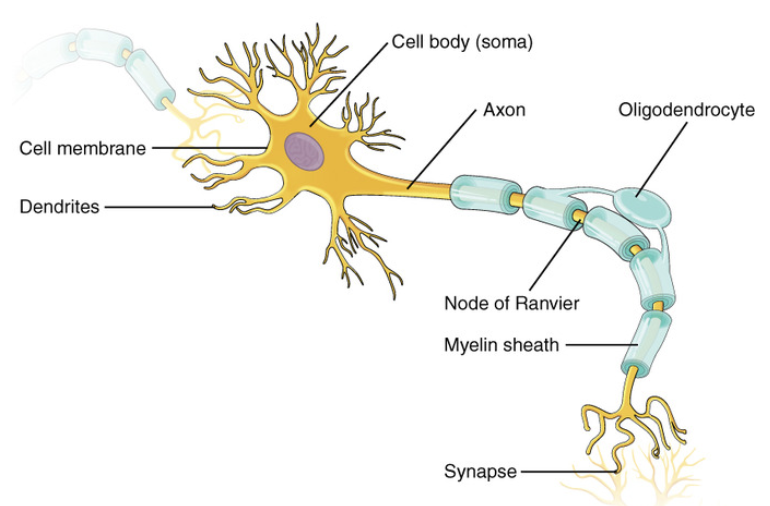
\includegraphics[width=0.7\textwidth]{neuron} % or use height= for vertical sizing
  \caption{Structure of a neuron \cite{Bond2022}.}
  \label{fig:neuron}
\end{figure}

To investigate white matter degeneration, we need tools that can probe the brain's microstructure. For this purpose, the structural characteristics of white matter as a highly organized tissue can be exploited: individual axons contain aligned microtubules, and groups of axons running in the same direction form coherent fibre bundles \cite{Assaf2013}. This makes white matter an ordered and highly directional tissue.

Water is a major component of white matter and exists in both intracellular and extracellular spaces. Water molecules undergo random motion due to thermal energy, a process known as diffusion. In free water, diffusion occurs equally in all directions (isotropic diffusion). However, given the ordered structure of white matter, diffusion becomes anisotropic. Water diffuses more easily along the direction of the axons, while diffusion perpendicular to the axons is hindered by cell membranes and the myelin sheath \cite{Beaulieu2013}. This is different from the surrounding tissues: in gray matter, diffusion is hindered equally in all directions, while in cerebrospinal fluid, it resembles free, isotropic diffusion.
This anisotropic diffusion is a distinctive feature of white matter, that can be exploited using Diffusion-weighted MRI. This non-invasive imaging technique enables the visualization of white matter fibre pathways and provides insights into their structure.

\section{Diffusion-weighted MRI}

 In free diffusion, molecular displacement follows a Gaussian distribution. According to Einstein's equation the mean displacement ($\sigma$=$\sqrt{2Dt}$) increases with both the diffusion coefficient D and the diffusion time t \cite{Mori20143}. In such conditions, the probability of diffusing of a given distance is equal in all directions, so diffusion is isotropic.
In biological tissues, however, water molecules encounter barriers such as cell membranes, which hinder their movement and reduce their diffusion displacement. As a result, the diffusion coefficient is lower than in free water and is referred to as the apparent diffusion coefficient (ADC). The ADC is influenced by the tissue's microscopic structure. In white matter (WM), diffusion is not isotropic: water molecules face more obstacles when moving perpendicular to axonal fibres than when moving along them. This directional dependence means a single diffusion coefficient is insufficient to describe water diffusion in WM and the ADC depends on the measurement direction.

 dMRI enables the investigation of tissue microstructure by measuring water molecule displacements. By quantifying ADC in multiple directions, with dMRI we can infer the orientation of WM fibres. Water molecules thus act as probes, revealing the tissue's microstructure and enabling the mapping of WM tracts, assuming diffusion is greatest along the direction of the fibre bundles \cite{LeBihan2003}. As such, dMRI is a valuable tool for studying WM anatomy and detecting pathological changes.

In MRI, image intensity depends on water concentration (proton density) and signal relaxation times. To make the signal sensitive to water diffusion, a pair of magnetic field gradient pulses can be applied. These gradients have an intensity that varies along a certain direction and are applied for a short period of time, 1-100ms.
When protons are placed in a magnetic field ${\ B}_0$, they acquire a precessing frequency proportional to the field strength, as described by the Larmor equation \cite{Jones2013}: 
\begin{equation}
\omega = \gamma{\ B}_0
\end{equation}

where $\gamma$ is the gyromagnetic ratio (2.7653108 rad/s$\cdot{T}$).
In a dMRI measurement, at first, all protons experience the same ${\ B}_0$, so they have the same frequency and phase. When the first gradient (called dephasing gradient) is applied, the magnetic field becomes position-dependent, causing protons to resonate at slightly different frequencies. In essence, the gradient "labels" the molecules by assigning them frequencies based on their spatial location. Once the gradient is switched off, all protons return to precessing at the same base frequency, but they now possess different phases. After a time $\Delta$, the second gradient (rephasing gradient) is applied. This gradient has the same amplitude and duration as the first one but with the opposite sign (or the same sign in the case of a spin-echo sequence, where a $180^\circ$ refocusing pulse is applied) \cite{Mori20142}.  When this second gradient is turned off, all protons again precess at the same frequency. If a molecule remained at exactly the same position during the interval $\Delta$, the phase shift induced by the first gradient is canceled by the second, and the net phase difference becomes zero.

However, because water molecules diffuse naturally, their positions are likely to change during $\Delta$. As a result, the phase shifts from the two gradients don't fully cancel out. The distribution of molecular displacements governed by the ADC leads to a distribution of phase shifts, which causes a loss of signal coherence. This dephasing reduces the total signal generated by all the protons \cite{LeBihan2003}. Therefore, by measuring the amount of signal attenuation caused by diffusion gradients, we can estimate the ADC. A greater spread of molecular displacements, corresponding to a higher ADC, results in greater signal attenuation \cite{Jones2013}. The ADC is not unique but depends on the direction in which the diffusion-sensitizing gradients are applied. 


\begin{figure}[h]
  \centering
  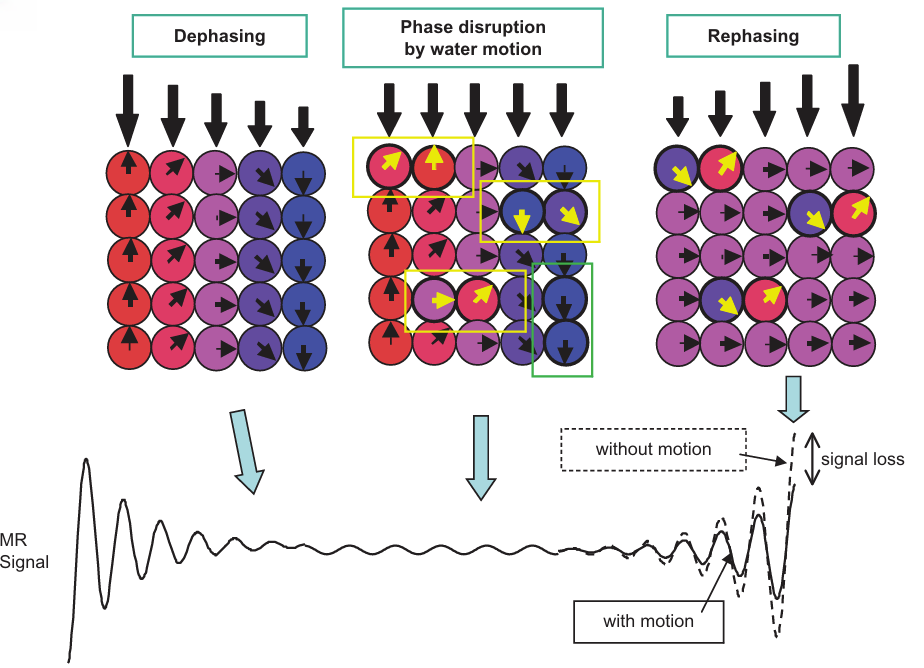
\includegraphics[width=0.7\textwidth]{Images/diffusion_2.png} % or use height= for vertical sizing
  \caption{Effect of dephasing and rephasing gradients on the phase of the spins. During dephasing and rephasing the magnetic field varies linearly with position (as indicated by the thick black arrows). The phase of the spins is indicated by the small arrows. Arrows in yellow indicate nuclei that diffuse in the gradient direction causing a net phase difference and consequently signal loss. In green, spins diffuse in the direction perpendicular to the gradient, causing no effect on the MR signal \cite{Mori20141}.}
  \label{fig:diffusion2}
\end{figure}



The values of ADC in a voxel reflect the underlying microstructure of the tissue. For example, in a voxel containing cerebrospinal fluid (CSF), the ADC is almost the same in all directions and fairly high, since diffusion is unrestricted. In contrast, within a WM voxel containing aligned fibre bundles, the ADC is significantly higher along the direction of the axons, and much lower in perpendicular directions due to restricted diffusion.

The typical spatial resolution of a diffusion-weighted MR image is on the order of a few millimeters, whereas the average displacement of water molecules during the measurement is between 1-20$\mu$m \cite{Mori20141}. As a result, the intensity of a diffusion-weighted image reflects the sum of many small contributions occuring at the microscopic scale.


The amount of signal loss is expressed as $\frac{S}{S_0}$, with $S_0$ the signal without diffusion weighting and S the measured signal, and it can be described by the equation:

\begin{equation}
\label{sig_att}
\frac{S}{S_0}=e^{-\gamma^2\cdot G^2\cdot\delta^2\cdot(\mathrm{\Delta}-\frac{\delta}{3})\cdot A D C}=e^{-b\cdot A D C}\
\end{equation}

where G and $\delta$ are the strength and length of the gradients. The signal loss increases with $\Delta$ and ADC, but also with G and $\delta$, as stronger or longer gradients determine more initial dephasing. G, $\Delta$, and $\delta$ are experimental parameters, while ADC is the quantity we want to estimate from the observed signal attenuation. The experimental parameters are combined into one parameter, the b-value, with units of $s/mm^{2}$. A higher b-value leads to greater signal attenuation.

\begin{figure}[h]
  \centering
  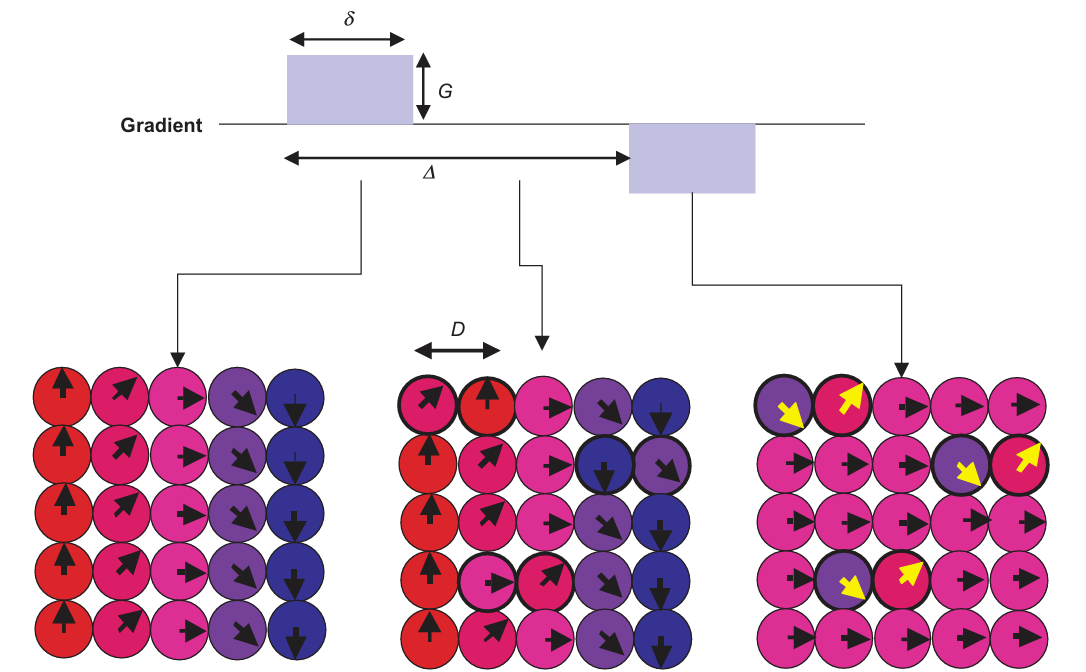
\includegraphics[width=0.7\textwidth]{Images/diffusion_1.png} % or use height= for vertical sizing
  \caption{Parameters of diffusion weighting ($\delta$, $G$, $\Delta$, D or ADC)\cite{Mori20142}.}
  \label{fig:diffusion1}
\end{figure}


 Taking the natural logarithm of the equation \eqref{sig_att} yields a linear relationship \cite{Mori20142}:

\begin{equation}
ln{(}\frac{S}{S_0})=-b\cdot ADC 
\end{equation}

This equation contains two unknowns: $S_0$ and ADC. Therefore, at least two measurements with different b-values are required to solve for ADC in a given gradient direction. In practice, more measurements are typically acquired to improve the signal-to-noise ratio (SNR), and a least squares fitting approach is used to estimate the parameters.

\section{Diffusion Tensor Imaging}
When diffusion is measured in complex, organized biological tissues such as WM, a single ADC value is insufficient to describe the behavior of water, as diffusion varies depending on the direction of measurement. To account for this anisotropy, a more sophisticated model called diffusion tensor imaging (DTI) was introduced \cite{ODonnell2011}. DTI models diffusion in each voxel as a 3x3 symmetric, positive-definite matrix known as the diffusion tensor, which captures the directional dependence of diffusion:

\[
D =
\begin{bmatrix}
D_{xx} & D_{xy} & D_{xz} \\
D_{xy} & D_{yy} & D_{yz} \\
D_{xz} & D_{yz} & D_{zz}
\end{bmatrix}
\]

The diffusion tensor contains six independent components, so at least six non-collinear, non-coplanar diffusion-weighted measurements are required, along with one unweighted reference image ($b$ = 0). Linear regression is then applied to the log-transformed diffusion signals to estimate the tensor components. In practice, more directions are often acquired to improve the robustness of the estimation using least squares fitting.

The diagonal elements of the tensor correspond to the diffusion coefficients along the three orthogonal axes, while the off-diagonal elements represent correlations between displacements along those axes. The tensor can be seen as a covariance matrix of molecular displacements \cite{Jones2013}, and it can be visualized as an ellipsoid. The surface of the ellipsoid represents the distance a water molecule, starting at the center, is likely to diffuse in each direction.
In the case of isotropic diffusion, where diffusion is equal in all directions, the ellipsoid becomes a sphere. In anisotropic diffusion, such as aligned WM fibres, diffusion is greater along one direction, and the ellipsoid becomes elongated along its principal axis. The principal axes of the ellipsoid are the eigenvectors of the diffusion tensor, and the lengths of these axes are proportional to the square roots of the eigenvalues ($\lambda_1$, $\lambda_2$, $\lambda_3$).

\begin{figure}[h]
  \centering
  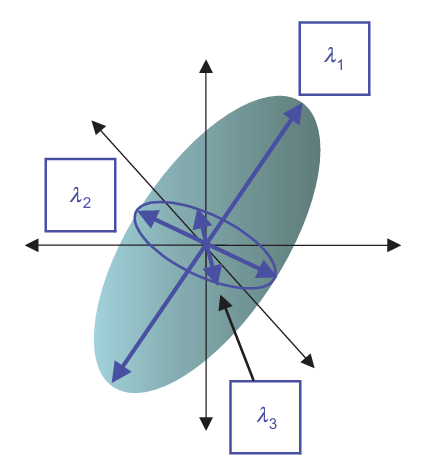
\includegraphics[width=0.6\textwidth]{Images/tensor.png} % or use height= for vertical sizing
  \caption{Diffusion tensor representation as an ellipsoid \cite{Mori20144}.}
  \label{fig:tensor}
\end{figure}

Several metrics can be derived from DTI. One widely used index is fractional anisotropy (FA), which quantifies the degree of anisotropy in a voxel:

\begin{equation}
\mathrm{FA} = \sqrt{\frac{3}{2}} \cdot \frac{\sqrt{(\lambda_1 - \bar{\lambda})^2 + (\lambda_2 - \bar{\lambda})^2 + (\lambda_3 - \bar{\lambda})^2}}{\sqrt{\lambda_1^2 + \lambda_2^2 + \lambda_3^2}}
\label{eq:FA}
\end{equation}

With $\bar{\lambda}$ the mean of the three eigenvalues. FA is defined as the normalized variance of the tensor's eigenvalues: it equals 0 in the case of isotropic diffusion and approaches 1 when diffusion is highly directional \cite{Jones2013}. FA quantifies the distance of the ellipsoid from a perfect sphere and is often interpreted as a measure of WM integrity.
Another commonly used metric is mean diffusivity (MD), calculated as the average of the tensor's eigenvalues.
MD provides a direction-independent measure of total diffusion within a voxel and is typically high in regions with free diffusion, such as cerebrospinal fluid \cite{LeBihan2001}.

As previously noted, diffusion MRI captures macroscopic signals that result from the aggregate effect of microscopic diffusion processes. This scaling difference between the physical phenomenon and what we can measure complicates the interpretation of voxel-wise metrics \cite{ODonnell2011}. At the same time, for microscopic phenomena to manifest at a larger scale, some degree of macroscopic structural coherence is required. This coherence influences which microstructural features can be detected using dMRI \cite{Mori20144}.

Information extracted from the diffusion tensor can also be used for tractography. Tractography is a method to estimate the trajectories of the fibre tracts in WM \cite{Lazar2010}. A common approach is streamline tractography, which works by successively stepping in the direction of the principal eigenvector (the direction of fastest diffusion) to reconstruct the tracts.

\section{Multi-shell Multi-tissue Constrained Spherical Deconvolution}

\subsection{DTI limitations}
One major limitation of DTI is its inability to resolve multiple fibre orientations within a single voxel, commonly referred to as crossing-fibres \cite{Seunarine2013}. Because DTI models diffusion using a second-order (rank-2) tensor, it can capture only one dominant diffusion direction per voxel. However, in many WM regions, the diffusion signal arises from more complex fibre geometries, such as crossing, kissing, or fanning fibres, which cannot be accurately represented by this simple model. In such cases, the diffusion tensor becomes not only inadequate but potentially misleading, compromising tractography results and undermining the interpretation of microstructural metrics like FA. A clear example of this limitation is the reported presence of low FA regions in deep white matter \cite{Mori20148}. These areas often contain two or more fibre populations oriented in different directions. Since DTI can only represent a single peak, it averages the signals from different directions, reducing the measured anisotropy and potentially leading to misinterpretation. An example can be seen in Figure~\ref{fig:crossing}.

\begin{figure}[h]
  \centering
  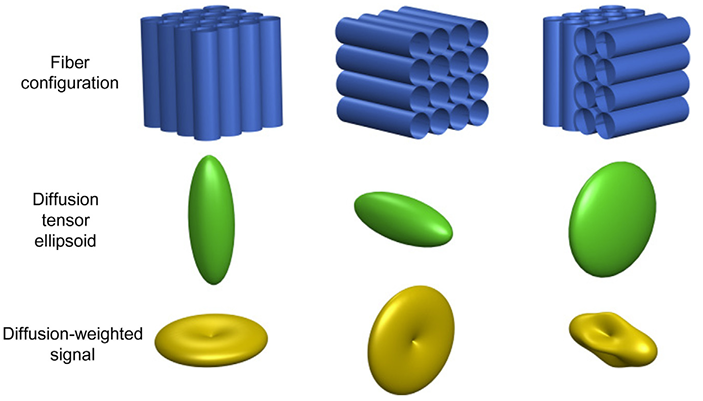
\includegraphics[width=0.7\textwidth]{Images/crossing.png} % or use height= for vertical sizing
  \caption{Example of how DTI can correctly recover the direction of fibres when only one fibre family is present (left and centre), but fails when two crossing families are present (right)\cite{Mori20148}.}
  \label{fig:crossing}
\end{figure}

\subsection{High angular resolution diffusion imaging}
This crossing fibres issue is highly relevant, as it is estimated that approximately 90\% of WM voxels contain more than one fibre population \cite{Jeurissen2013}. This limitation becomes critical in clinical applications such as neurosurgical planning, where tractography based on DTI may fail to identify important fibre bundles. Such false negatives could lead to incorrect conclusions about which brain regions are safe to operate on.

To address these limitations, methods are needed that can model multiple fibre populations within a voxel. To characterize the DW signal more exhaustively, High Angular Resolution Diffusion Imaging (HARDI) is employed \cite{Descoteaux2015}. HARDI is a data acquisition protocol that involves sampling the diffusion signal with many gradient directions uniformly distributed over a sphere for each b-value. Typically, the same set of directions is used across different b-values, forming multiple acquisition "shells".

This high angular sampling allows the angular features of the diffusion signal to be captured with finer resolution. Using multiple b-values further enhances the characterization of the signal, although it increases scan time. For DTI, the optimal b-value is generally around 1000 s/${mm}^{2}$, but for higher-order models that employ HARDI, the ideal b-value is less well-defined \cite{Mori20148}. Higher b-values improve the ability to resolve fibre orientations but also result in greater signal attenuation, reducing the SNR.
With HARDI data, it is possible to compute fibre orientation distribution functions (fODFs or simply ODFs). These functions describe the distribution of fibre orientations within a voxel. Defined over the unit sphere, the ODF assigns to each direction the probability of finding a fibre population aligned with it \cite{Seunarine2013}.

\subsection{Constrained Spherical Deconvolution}

A common method to recover the ODF from the diffusion signal is spherical deconvolution \cite{DellAcqua2019}. The core idea is to model the signal in each voxel as a combination of scaled and reoriented versions of a response function, the expected diffusion signal generated by a single, coherently oriented fibre population. The scaling is given by the fraction of fibres belonging to a certain family and the reorientation is needed to align the response with the fibre direction. The response function is typically derived by averaging the diffusion signal from voxels that are highly anisotropic and are presumed to contain only one dominant fibre orientation \cite{Tournier2007}. These signals are realigned to a common reference direction before averaging.

Mathematically, the total diffusion signal in a voxel is modeled as the convolution of this response function with the ODF, as shown in Figure~\ref{fig:convolution}.

\begin{figure}[h]
  \centering
  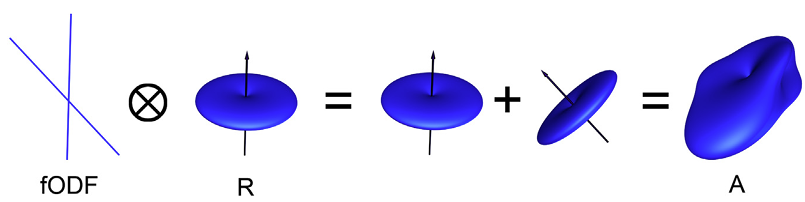
\includegraphics[width=0.7\textwidth]{Images/convolution.png} % or use height= for vertical sizing
  \caption{Convolution of the fODF with the response function R to obtain the measured diffusion-weighted signal A \cite{Seunarine2013}.}
  \label{fig:convolution}
\end{figure}

By inverting the operation, through spherical deconvolution, the ODF can be recovered. However, spherical deconvolution is an ill-posed problem, which could result in spurious peaks or negative values. To address this, regularization is applied, resulting in constrained spherical deconvolution (CSD). CSD imposes constraints to suppress physically implausible negative values and ensure a more reliable estimate of the ODF. For a single shell, CSD can be formulated as a constrained least squares problem \cite{Jeurissen2014}:

\begin{equation}
\hat{\boldsymbol{x}} = \arg\min_{\boldsymbol{x}} \frac{1}{2} \| C\boldsymbol{x} - \boldsymbol{d} \|_2^2 \quad \text{subject to} \quad A\boldsymbol{x} \geq \boldsymbol{0}
\label{eq:CSD}
\end{equation}

where $\boldsymbol{x}$ is the vector of coefficients of the ODF, $\boldsymbol{d}$ the vector of measured signal intensities, $C$ the matrix relating $\boldsymbol{x}$ to $\boldsymbol{d}$ by means of spherical deconvolution, and $A$ the matrix relating the ODF coefficients to their amplitudes.
CSD can effectively recover multiple fibre orientations within a voxel. An example of an ODF recovered using CSD in in Figure~\ref{fig:odf}. The peaks of the estimated ODF correspond to directions with the highest probability of having a fibre bundle, and the peak amplitudes are proportional to the underlying fibre density.
\\The use of ODFs has been shown to improve the reliability of tractography results when compared to traditional DTI methods \cite{Jeurissen2011}.

\begin{figure}[h]
  \centering
  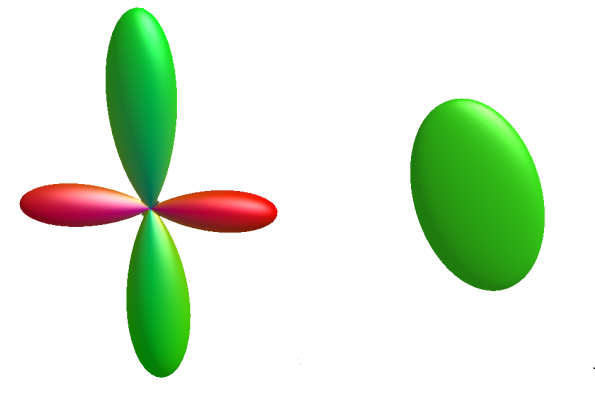
\includegraphics[width=0.5\textwidth]{Images/odf.png} % or use height= for vertical sizing
  \caption{An example of a fODF as recovered through CSD with the corresponding diffusion tensor next to it. The RGB color convention used to represent the directionality is red for right-left, blue for dorsal-ventral, and green for anterior-posterior.}
  \label{fig:odf}
\end{figure}

\subsection{Multi-shell multi-tissue CSD}
A more advanced model is Multi-Shell Multi-Tissue CSD (MSMT-CSD) \cite{Jeurissen2014}, which addresses limitations of single-tissue, single-shell CSD. Single-response models are accurate primarily in voxels containing pure WM, but can lead to overestimation of WM in voxels with mixed tissue types. MSMT-CSD addresses this by using multi-shell data and distinct response functions for different tissue types, typically WM, gray matter (GM), and cerebrospinal fluid (CSF). This approach not only estimates the fODF but also provides tissue-specific signal fractions within each voxel.
In MSMT-CSD, response functions are modeled using spherical harmonics (SH). The WM response function is assumed to be anisotropic and is modeled using a SH series of higher order, typically order 8 corresponding to 45 coefficients (Figure~\ref{fig:response}), while GM and CSF are modeled as isotropic and represented with SH series of order 0. Each response function is estimated separately for each b-value shell. 
Equation~\ref{eq:CSD} is extended to support m shells and n tissue types as follows:

\begin{equation}
\begin{bmatrix}
\hat{\boldsymbol{x}}_1 \\
\vdots \\
\hat{\boldsymbol{x}}_n
\end{bmatrix}
=
\arg\min_{\boldsymbol{x}}
\frac{1}{2}
\left\lVert
\begin{bmatrix}
{C}_{1,1} & \cdots & {C}_{1,n} \\
\vdots & \ddots & \vdots \\
{C}_{m,1} & \cdots & {C}_{m,n}
\end{bmatrix}
\begin{bmatrix}
\boldsymbol{x}_1 \\
\vdots \\
\boldsymbol{x}_n
\end{bmatrix}
-
\begin{bmatrix}
\boldsymbol{d}_1 \\
\vdots \\
\boldsymbol{d}_m
\end{bmatrix}
\right\rVert_2^2
\end{equation}

\[
\text{subject to } 
\begin{bmatrix}
{A}_1 & 0 & 0 \\
0 & \ddots & 0 \\
0 & 0 & {A}_n
\end{bmatrix}
\begin{bmatrix}
\mathbf{x}_1 \\
\vdots \\
\boldsymbol{x}_n
\end{bmatrix}
\geq 0
\]


Voxels dominated by a specific tissue type are selected to derive response functions. Originally, supervised approaches were used to define these voxels based on T1-weighted images and registration. More recently, unsupervised methods relying solely on diffusion data by analyzing signal decay and FA values have been developed and shown to improve accuracy \cite{Raffelt2016}.
\begin{figure}[h]
  \centering
  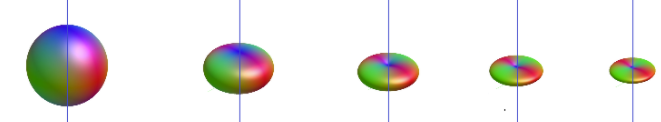
\includegraphics[width=0.5\textwidth]{Images/response.png} % or use height= for vertical sizing
  \caption{WM response function for 5 shells. With b=0 (no diffusion weighting) the response is isotropic, then with increasing b-value the signal is attenuated especially in the fibre direction.}
  \label{fig:response}
\end{figure}

MSMT-CSD is a powerful approach that can model multiple fibre orientations in each voxel with minimal assumptions, relying exclusively on diffusion data. It improves upon previous methods by using more data through incorporating multiple shells, and accounting for partial volume effects due to different tissue types.
However, limitations remain. The estimation of the response functions is largely heuristic, and the method relies on the assumption that a single average response function adequately represents all fibre populations across the brain. In reality, fibre characteristics such as configuration, cell size, and density may vary regionally \cite{Seunarine2013}. This is partially accounted for through ODF normalization \cite{Dhollander2021}, but some of the effects remain. Additionally, the standard three-tissue model does not account for atypical or pathological tissue types, which could lead to wrong results in brains affected by disease.

\section{Local Response Function estimation in Spherical Deconvolution}

To address the limitations of MT-CSD, a new method has been proposed: Local Response Function Estimation in Spherical Deconvolution (LoRE-SD). This approach eliminates the need for heuristic, global response function estimation by determining a voxel-wise response function directly from the data. As a result, the assumption that fibre populations generate the same signal across all brain regions is no longer required, making LoRE-SD more suitable for cases involving pathology or tissue types beyond the conventional WM, GM, and CSF classes.
\\In LoRE-SD, the response function in each voxel is modeled as a weighted sum of Gaussian basis functions, which are dependent on both the b-value ($b$) and the angle between the diffusion gradient direction and the fibre orientation ($\alpha$). These basis functions are parametrized by axial and radial diffusivity, and can be organized on a 10x10 grid representing all combinations of these two parameters, as shown in Figure~\ref{fig:grid}. Only the lower triangle of this grid is used, as the radial diffusivity must not exceed axial diffusivity.
Each Gaussian basis function is described as:

\begin{equation}
G_{\lambda_{\parallel}, \lambda_{\perp}}(b, \alpha) = 
e^{-b \lambda_{\perp}} \, 
e^{-b (\lambda_{\parallel} - \lambda_{\perp}) \cos^2 \alpha}
\end{equation}

Where $\lambda_{\parallel}$ and $\lambda_{\perp}$ are the axial and radial diffusivities.

\begin{figure}[h]
  \centering
  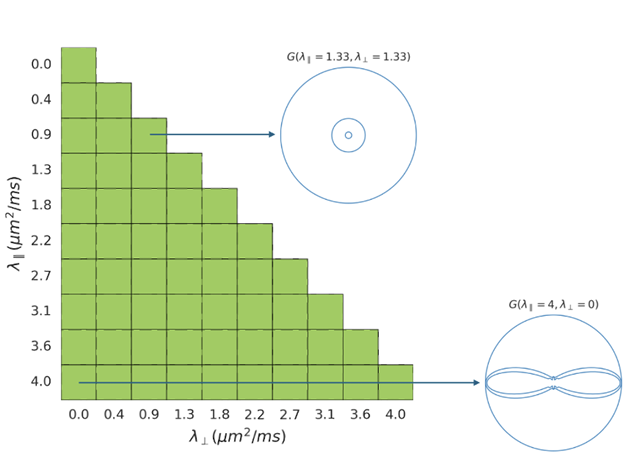
\includegraphics[width=0.7\textwidth]{Images/grid.png} % or use height= for vertical sizing
  \caption{Grid showing the Gaussian basis functions used to describe the response functions in LoRE-SD. $\lambda_{\parallel}$ and $\lambda_{\perp}$ are the axial and radial diffusivities.}
  \label{fig:grid}
\end{figure}

During optimization, in each voxel the method assigns a weight $f_{\lambda_\parallel, \lambda_\perp}$ to each basis function (Gaussian fractions). At each iteration, both the $f_{\lambda_\parallel, \lambda_\perp}$ and the SH coefficients of the ODF are estimated simultaneously for each voxel. The optimization problem is formulated as:

\begin{equation}
\min_{F, R} \quad \sum_{\ell \in \{0,2,\dots,\ell_{\max}\}} \left(S_\ell - \mathcal{N}_\ell R_\ell F_\ell^\top \right)^2 + \lambda \sum_{b,\ell>0} R_{b,\ell}^2
\end{equation}

Subject to:

\begin{equation}
F_0 = \frac{1}{\sqrt{4\pi}}
\end{equation}

\begin{equation}
Q F^\top \geq 0
\end{equation}

\begin{equation}
R = S_0 \sum_{\lambda_\parallel = 0}^{\lambda_\parallel^{(\max)}} \sum_{\lambda_\perp = \lambda_\parallel}^{\lambda_\perp^{(\max)}} f_{\lambda_\parallel, \lambda_\perp} G_{\lambda_\parallel, \lambda_\perp}
\quad \text{with} \quad 0 \leq f_{\lambda_\parallel, \lambda_\perp} \leq 1
\end{equation}

\begin{equation}
\sum_{\lambda_\parallel = 0}^{\lambda_\parallel^{(\max)}} \sum_{\lambda_\perp = \lambda_\parallel}^{\lambda_\perp^{(\max)}} f_{\lambda_\parallel, \lambda_\perp} = 1
\end{equation}

where $F$ represents the ODF, $R$ the response function and $S$ the diffusion signal. $\mathcal{N}_\ell$ is a normalization factor ($\frac{4\pi}{2\ell + 1}$) and $Q$ is a transformation matrix from spherical harmonics to spherical coordinates. $\lambda$ is a regularization parameter, usually $10^{-3}$ and $l$ represents the SH order. $l_{max}$ is usually set to  8.
A non-negativity constraint is imposed to the ODF (as for previous CSD methods) and the regularization term is used to promote isotropic response functions.
The ODFs generated by LoRE-SD are unit-normalized, meaning that, unlike the WM ODF resulting from MT-CSD, the amplitudes of their lobes do not inherently reflect fibre density. To assign meaningful magnitudes to the lobes, a scaling factor is required. This can be achieved using a contrast matrix, where each Gaussian basis function is assigned a weight (from 0 to 1) to emphasize or suppress specific basis functions. For example, a contrast matrix mimicking intra-axonal compartment can be obtained assigning high weights to basis functions with high axial and low radial diffusivity, with an exponential decay as radial diffusivity increases.
A contrast image is then computed for each voxel by taking the inner product between this contrast matrix and the basis function weights estimated in that voxel. This produces a scalar value per voxel, which is higher when the local signal aligns well with the response function described by the contrast matrix. An example for the described intra-axonal contrast is in Figure~\ref{fig:contrast}. These contrast images can then be used as voxel-wise scaling factors for the ODFs, assigning meaning to the amplitude of the lobes. Different contrast matrices can be designed depending on the tissue features of interest. 

\begin{figure}[h]
  \centering
  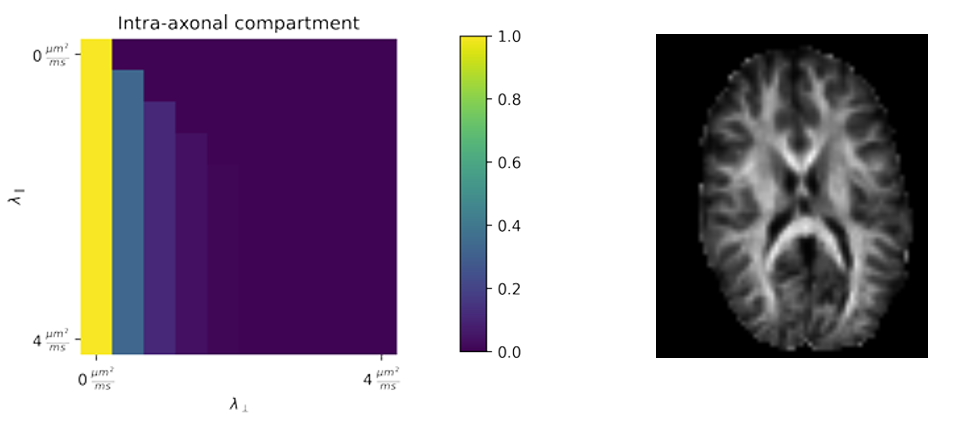
\includegraphics[width=0.7\textwidth]{Images/contrast.png} % or use height= for vertical sizing
  \caption{Contrast matrix used to define the intra-axonal contrast and example of the resulting contrast for one subject.}
  \label{fig:contrast}
\end{figure}

\section{Fixels}

DTI-derived metrics, such as FA, are widely used in voxel-based analysis (VBA) \cite{Liu2009}, where each voxel is assigned a scalar value and group-level statistical comparisons are performed. These studies can be cross-sectional (comparing different groups) or longitudinal (assessing changes over time, for example, due to disease progression). However, a key limitation of VBA is that it assigns a single scalar value per voxel, ignoring the fact that different fibre populations within a voxel may behave differently. This limitation reduces the biological specificity and interpretability of the results.
\\As mentioned, one of the main advantages of higher-order diffusion models like CSD is their ability to resolve complex fibre configurations, such as crossing fibres. By representing multiple fibre populations separately within a voxel, ODFs allow the extraction of fibre bundle-specific quantitative information, associating values not to the voxel but to the specific fibre orientations. In the previous sections, we described two methods for obtaining ODFs. In the first case (MT-CSD), the amplitude of the ODF lobes is intrinsically related to the apparent fibre density of the corresponding fibre population. In the second case (LoRE-SD), this relationship can be re-established by applying an appropriate scaling contrast, such as the intra-axonal compartment contrast.
\\To enable group-level analysis of this fibre-specific information, an important step is the extraction of fixels \cite{Raffelt2017}. A fixel is defined as a single fibre population within a voxel. Fixels are extracted by identifying the direction of each ODF lobe peak, with only those above a certain amplitude threshold retained to reduce the inclusion of spurious or noisy peaks. Each fixel is represented as a line segment passing through the center of the voxel, as the actual position of the fibre family within the voxel cannot be known. The information is in the directionality, while the length has no meaning. A single voxel can contain multiple fixels, or none at all, depending on the underlying fibre structure. An example of ODFs and the extracted fixels is shown in Figure~\ref{fig:fixel}. Taking inspiration from VBA, a Fixel-Based Analysis (FBA) can be performed, assigning metrics to individual fixels rather than entire voxels \cite{Dhollander2021}. These fixel-wise metrics can reflect fibre-specific properties, potentially tied to only specific microstructural compartments within a voxel. However, working with fixels introduces new challenges, including registration, fixel correspondence across subjects, and statistical inference. These topics, along with the detailed FBA pipeline, will be discussed in the next section.

\begin{figure}[h]
  \centering
  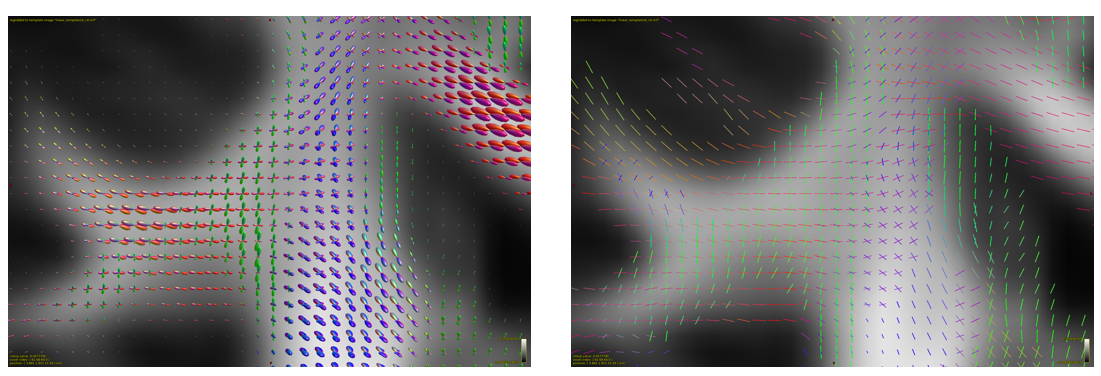
\includegraphics[width=0.8\textwidth]{Images/fixel.png} % or use height= for vertical sizing
  \caption{Left: WM ODFs found with MSMT-CSD. Right: corresponding fixels. In both images the colors represent the directionality. The RGB color convention used is red for right-left, blue for dorsal-ventral, and green for anterior-posterior.}
  \label{fig:fixel}
\end{figure}

\section{Fixel Based Analysis}
\label{sec:fba}
Below, we outline the metrics used in FBA and the standard pipeline that starts from WM ODFs derived from MT-CSD, before describing the changes introduced by LoRE-SD in a later section.

\subsection{Apparent Fibre Density}
The first fixel-wise metric derived from a WM ODF is Apparent Fibre Density (AFD) \cite{Raffelt2012}. This metric is calculated by numerically integrating the amplitude of the ODF lobe along a given direction using dense angular sampling \cite{Smith2013}. The amplitude of the ODF in a specific orientation is proportional to the DW signal perpendicular to that orientation, which in turn reflects the intra-axonal water fraction, or in other words, the density of the fibres.
Since ODF amplitude is influenced by both the underlying fibre population and the response function used during deconvolution, in a study it is critical to use a common response function across all subjects. This ensures consistent scaling of the ODFs, making inter-subject comparisons meaningful. A typical strategy involves averaging the response functions across all subjects to obtain a study-specific response function.
AFD is influenced both by axon count and axon diameter \cite{Dhollander2021} and it can be interpreted as a the fibre bundle's capacity to transfer information \cite{Raffelt2012}. However, AFD is also affected by the presence and the changes of other fibre populations or other tissue compartments in the same voxel, which can confound the interpretation.

\subsection{Intensity normalization and bias field correction}
An essential step in MT-CSD-based FBA is intensity normalization, which aims to make AFD values comparable across subjects \cite{Raffelt17}. This step ensures that the total diffusion signal, summed across all tissue compartments, remains approximately constant throughout the brain. This assumption helps correct for bias fields and for the fact that a single response function may not be representative of the whole brain. After normalization, the WM, GM, and CSF ODFs are scaled to comparable units.

\subsection{Template Construction and Registration}
Group analysis begins with the creation of a study-specific template. This is typically built using ODFs from a representative subset of subjects (excluding anatomical outliers). After initialization with an initial average image, the construction follows an iterative process:

\begin{enumerate}
    \item Registration of each subject to the template.
    \item Template update as the mean of the registered images.
\end{enumerate}

A possible approach is using rigid registration for the first iterations, then affine, and finally nonlinear.
Higher order information contained in the ODFs has been shown to improve the results of registration, compared to FA- or T1-based methods \cite{Raffelt2011}. At each iteration, each ODF is spatially transformed, interpolated and then reoriented using local angular transformations. This last step ensures that the orientation information remains anatomically correct with respect to the new spatial configuration.
ODF reorientation is performed using a point spread function (PSF) model: the ODF is approximated as a sum of PSFs, each of which is transformed individually. The transformed PSFs are then summed to obtain the final reoriented ODF \cite{Raffelt12}. A diffeomorphic transformation is used to ensure that the Jacobian determinant remains positive, a necessary condition for proper ODF reorientation.

Once the ODF template is obtained, ODF-guided registration is used to move subjects data to the common space, which results is the nonlinear warps that will be used to extract the next metric. The transformation is applied, but roerientation is delayed to a later step. This means that the transformed ODF images are anatomically-broken.

\subsection{Fixel Extraction and Correspondence}
A fixel mask is generated by segmenting the template ODFs. Only lobes above a certain amplitude threshold, indicative of consistent fibre presence across subjects, are retained. The amplitudes are lower were subject ODFs align less well, for example at the GM/WM interface where the inter-subject variation is high and registration is imperfect.

Then for each subject:

\begin{enumerate}
    \item Fixels are extracted from their WM ODFs in template space.
    \item Fixels are reoriented using the nonlinear warp.
    \item AFD values are computed by integrating the amplitude of each valid lobe and are assigned to the corresponding fixel.
\end{enumerate}

Fixel correspondence between subject and template is established by searching, within each voxel, for matching fixels in the template (within an angular threshold). If no match is found, the AFD value is set to zero for that fixel in that subject.

\subsection{Fibre-Cross Section}
An additional metric that can be derived directly from the spatial warp fields is the Fibre Cross-Section (FC) \cite{Raffelt2017}. The nonlinear warp used to register a subject to the template describes the local volume change, quantified by the determinant of the Jacobian matrix ($det( J)$). When analyzing WM fibres, only changes perpendicular to the fibre orientation are biologically meaningful, as they reflect alterations in the number of axons across a bundle's cross-section.

FC measures these perpendicular volume changes, providing complementary information to AFD and is defined as:
\begin{equation}
FC_f = \frac{det( J)}{\lVert J\hat{\boldsymbol v}_f\rVert}
\end{equation}

where the component in the direction of the fixel f (described by the unit vector $\hat{\boldsymbol v}_f$) is factored out from the total volume change.
This is a relative metric, as it describes the volume change relative to the template. This means that it can only be compared across subjects in the same study and only in corresponding brain regions.
While AFD reflects microstructural changes (the axonal density), FC captures macrostructural changes (the bundle size).

An additional metric can be derived as the fixel-wise product of AFD and FC, known as Fibre Density and Cross-section (FDC) \cite{Raffelt2017}. This metric provides a more comprehensive measure that accounts for both microscopic and macroscopic changes in WM. FDC can thus be interpreted as reflecting the total intra-axonal volume, combining information about the number of axons and their spatial distribution in the brain.
However, interpreting these three metrics is not always straightforward and must be contextualized within the underlying pathology. For instance, in a disease process that initially causes axonal loss, a reduction in AFD might be expected in the affected regions. But if atrophy occurs later, reducing the cross-sectional area of the tract, the remaining axons may become more densely packed, potentially leading to an unexpected increase in AFD. In such a scenario, FC would be reduced, and FDC might remain unchanged, emphasizing the importance of considering all three metrics together to accurately characterize pathological changes. A graphical example of this situation is in Figure~\ref{fig:atrophy}.
Finally, it is important to note that the separation between AFD and FC is not always clear-cut in practice \cite{Dhollander2021}. Due to the limitations of non-rigid image registration, part of an effect that should be attributed to FC may instead be attributed to AFD, and vice versa. This ambiguity is particularly pronounced in small or thin structures, and means that AFD and FC should not be directly compared in terms of effect size. Therefore, FDC is often a more reliable metric, as it incorporates both effects.\\

\begin{figure}[h]
  \centering
  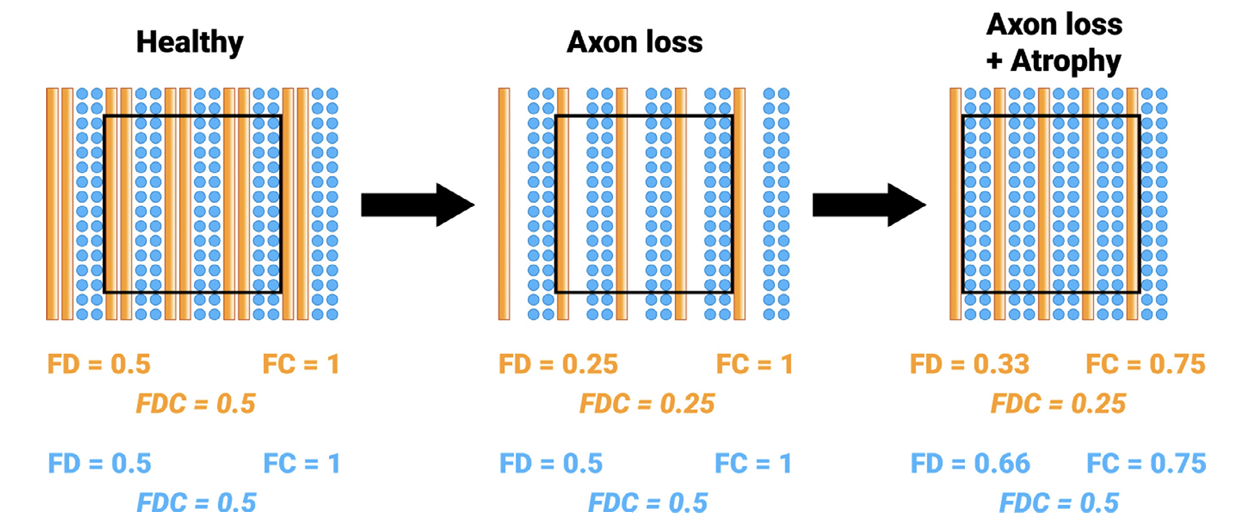
\includegraphics[width=0.8\textwidth]{Images/atrophy.png} % or use height= for vertical sizing
  \caption{Example of how the three metrics need to be considered together and that metrics related to one fibre family are influenced by the other components in the same voxel. By just considering AFD (FD) for the blue fibre family, one may conclude that the disease leads to an increase of the number of axons. But this is due to the atrophy as it can be inferred by the decrease of FC and the constant FDC. Additionally, even though AFD and FC change for the blue family, the disease didn't have a direct effect on the blue axons. The change is due to the blue fibres sharing the voxel with the affected orange fibres \cite{Dhollander2021}.}
  \label{fig:atrophy}
\end{figure}

In VBA, once anatomical correspondence between subjects is established through registration, the next steps are smoothing the images, performing voxel-wise statistical testing, and assigning p-values based on statistical inference \cite{Raffelt2015}. These steps must be adapted for FBA, as fixels in neighboring voxels may belong to different fibre populations and comparisons need to be fixel-wise.

\subsection{Smoothing Using Structural Connectivity}
In VBA, smoothing of the metrics is typically applied using a Gaussian kernel centered on each voxel, averaging across neighboring voxels to improve SNR, reduce registration errors, and increase robustness. However, this method is not directly applicable to fixels because adjacent voxels may contain unrelated fibre populations. Instead, FBA requires a smoothing strategy that respects WM tract architecture. To achieve this, a whole-brain probabilistic tractography is generated on the ODF template. This is used to define structural connectivity between all fixels, resulting in a fixel-fixel connectivity matrix \cite{Raffelt2015}. This is a sparse matrix where each element $c_{ij}$ is the proportion of streamlines passing through fixel i that are also passing through fixel j. These values are combined with a Gaussian kernel centered at the fixel of interest to weight the contribution of structurally connected fixels during smoothing. This ensures that only anatomically connected fixels influence one another.

\subsection{Statistical Testing and Inference in FBA}

As in VBA, statistical inference in FBA must address the problem of multiple comparisons. A popular solution for VBA relies on the idea that true positives will form spatially coherent clusters, as the underlying anatomy or pathology is shared among them. This is known as cluster-based inference \cite{Winkler2014}. Threshold-Free Cluster Enhancement (TFCE) avoids choosing an arbitrary threshold for forming clusters by integrating across all thresholds, resulting in an enhanced test statistic that reflects both the original test statistic values and the spatial extent of the clusters.

An approach inspired by TFCE but adapted for FBA is connectivity-based fixel enhancement (CFE) \cite{Raffelt2015}. CFE uses the fixel-fixel connectivity matrix to define clusters of structurally connected fixels and enhance the statistical power. The connectivity information is used to weight contributions from neighboring fixels when computing the enhanced test-statistic: fixels more structurally connected to the one of interest contribute more strongly. The goal is to recover statistical power lost due to correction for multiple comparisons by assuming that changes in one fixel are likely to co-occur along structurally related WM pathways.

Statistical hypotheses in fixel-based analysis are typically framed within a general linear model (GLM). The GLM allows modeling each fixel-wise metric (AFD, FC, FDC) as a linear combination of explanatory variables (e.g., group, age), encoded in a design matrix. Model parameters are estimated, and statistical tests (t-tests) are performed at each fixel to assess the effects of interest.

Permutation testing is the preferred method for inference, as it reduces the number of assumptions. The only requirement is exchangeability under the null hypothesis \cite{Winkler2014}. This involves randomly permuting the data (e.g., reassigning group labels) and recalculating the test statistic for each permutation. The p-value is the proportion of permutations with a test statistic as extreme or more extreme than the observed one, which quantifies evidence against the null hypothesis.

To address the issue of multiple comparisons, permutation testing is also used to compute family-wise error (FWE) corrected p-values. This is done by recording the maximum test statistic across all fixels for each permutation, creating a distribution of maximal values. The FWE-corrected p-value for each fixel is then the proportion of permutations in which the maximum statistic exceeds the observed one. This approach is compatible with CFE: at each permutation the maximum cluster-enhanced test statistic is recorded.\\
Finally, statistically significant fixels can be identified as those with a FWE-corrected p-value below 5\%.

\section{FBA and LoRE-SD}
FBA can be extended to ODFs derived from LoRE-SD. Unlike MT-CSD ODFs, which require intensity normalization across subjects, LoRE-SD ODFs are unit-normalized by design. The first step is selecting a specific contrast which assigns a scaling factor to each ODF.

In MT-CSD, ODF lobe amplitudes are directly influenced by the response functions, with the WM response function acting as a "unit," thus enabling direct comparison across subjects. In LoRE-SD, however, the lobe amplitudes depend on the chosen contrast via the response function representation. Comparability across subjects is ensured by using the same contrast matrix for all. The metric resulting from integrating the ODF lobe, analogous to AFD, will reflect the chosen contrast. FC and FDC can be computed using the deformation fields (warps) obtained during registration to the population template, following the same steps as in the MT-CSD-based pipeline.

The most computationally intensive step of the FBA pipeline is creating the study-specific template via non-linear ODF registration. If different contrasts are applied to scale the ODFs, they only differ by a multiplicative constant at each voxel. This suggests that a template constructed with one contrast (e.g., intra-axonal) could potentially be reused with ODFs scaled using other contrasts. This is because the deformation fields (warps) represent spatial transformations, which should ideally be contrast-independent. In practice, however, the iterative nature of registration and template construction means that using a different contrast (or even re-registering with the same contrast) results in slightly different warps. As long as these discrepancies are small, the FBA pipeline compensates for them via smoothing, which is guided by the fixel-fixel connectivity matrix.\\ While it's possible to build the template from unscaled (unit-normalized) ODFs, this may be suboptimal, as registration would be driven purely by directional information. Scaled ODFs incorporate amplitude information, which can improve registration accuracy, particularly since the same contrast representation is used across subjects, making lobe amplitudes more or less consistent in corresponding brain regions.

So, using the same warps for differently scaled ODFs may be acceptable, with the main consequence being a change in the extracted AFD-like values. FC remains unchanged, as it depends solely on the warp fields. Consequently, the fixel correspondence between subject and template is preserved, and only the amplitude (integrated lobe value) associated with each fixel will vary. Employing multiple contrasts to scale the ODFs could be useful, as extracted metrics from each one could give us unique insights. As a result, statistical testing on AFD or FDC may be different depending on the contrast used to scale the ODFs. While FC remains unaffected, differences in amplitude scaling may influence effect sizes and statistical significance for the other two metrics.

\section{Chemobrain and Diffusion MRI}

Several studies have used DTI to investigate WM changes associated with chemotherapy, particularly on breast cancer patients. Matsos et al. \cite{Matsos2017} reported that chemotherapy-treated patients performed worse than healthy controls in tests of attention and psychomotor speed. These deficits were accompanied by reduced FA in frontal, occipital, and parietal WM tracts. Similarly, Deprez et al. \cite{Deprez2011} performed a study on breast cancer patients and observed decreased FA in frontal and temporal WM regions, along with increased MD in frontal tracts. Additionally, they found that lower FA values correlated with poorer cognitive test performance, particularly in the superior longitudinal fasciculus and inferior longitudinal fasciculus.

Longitudinal studies have offered additional insights. Chen et al. \cite{Chen2020} investigated older breast cancer patients ($\geq$60 years) before and within one month after chemotherapy. While no significant changes in FA were detected, they observed increased MD and radial diffusivity in the genu of the corpus callosum post-treatment. Another study by Koppelmans et al. \cite{Koppelmans2014} focused on long-term effects and found no significant differences in DTI metrics between healthy controls and breast cancer survivors. However, they did identify a negative correlation between time since treatment and WM integrity, with lower FA and higher MD over time.
Deprez et al. \cite{Deprez2012} conducted a longitudinal assessment of cognitive performance and DTI metrics again on breast cancer patients. Patients showed a decline in cognitive test scores 3-4 months after chemotherapy, along with decreased FA in frontal, parietal, and occipital WM tracts. These FA reductions correlated with performance declines, suggesting a link between treatment-induced WM changes and cognitive impairment. The observed microstructural alterations may reflect axonal injury or demyelination, both of which impact WM diffusivity.

FBA has also been employed to study the impact of chemotherapy. Schroyen et al. \cite{Schroyen2021} compared chemotherapy-treated breast cancer patients, non-chemotherapy patients, and healthy controls but found no significant group differences in fixel-wise metrics, possibly due to limited sample size. However, they identified a negative association between log-transformed FC (log-FC) in the corpus callosum and glial cell overexpression, indicating possible neuroinflammation. The corpus callosum, being densely packed with axons and highly vascularized, may be especially vulnerable to chemotherapy-induced damage.

\section{Aim of the Thesis}

The aim of this thesis is to apply the LoRE-SD method within a FBA framework and to compare the results with those obtained using the standard approach based on WM ODFs derived from MT-CSD. This will allow us to assess whether LoRE-SD is suitable for integration into the FBA pipeline. Furthermore, the flexibility introduced by LoRE-SD's scaling may enable the extraction of additional and potentially more meaningful microstructural information than with MT-CSD alone. Since FBA results depend on both the ODFs and the applied modulation, we will investigate whether different scaling strategies affect the significance and the distribution of the detected effects.
\\This analysis will be carried out in the context of a group study involving breast cancer patients undergoing chemotherapy, patients not receiving chemotherapy, and a control group of healthy subjects. An additional objective is to investigate whether chemotherapy induces detectable changes in WM. We hypothesize that significant group differences in fixel-wise metrics may be found, particularly in WM regions involved in memory and cognitive functions. Such differences may reflect disruption of WM integrity, potentially underlying the cognitive decline observed in some patients.



\chapter{Methods}
In this chapter, we describe the dataset, the dMRI acquisition and preprocessing steps, and brain mask extraction. We then outline the FBA pipeline with LoRE-SD–specific steps, highlight key parameters, and describe the statistical analysis, including strategies to increase statistical power by reducing the number of fixels.

\section{Dataset Description}
The dataset consists of 101 women divided into three groups: two breast cancer groups and one healthy control (HC) group. The first breast cancer group includes patients undergoing chemotherapy (CP), while the second group includes cancer patients not receiving chemotherapy (CM). Data were collected three months post-chemotherapy.

The principal characteristics of the subjects belonging to the three groups are described in \cref{tab:dataset}.

\begin{table}[H]
    \caption*{\textbf{Subject characteristics by group}} % visible bold title
    \centering 
    \begin{tabular}{|p{6em} c c|} % wider first column
    \hline
    \rowcolor{bluepoli!40} % comment this to remove the color
    \textbf{Group} & \textbf{Number of Subjects} & \textbf{Mean Age (SD)} \T\B \\
    \hline \hline
    CP & 28 & 50.36 (8.61) \T\B \\
    CM & 32 & 51.93 (7.15) \T\B \\
    HC & 41 & 47.46 (10.29) \B \\
    \hline
    \end{tabular}
    \\[10pt]
    \caption{Mean and standard deviation (SD) of age per group are indicated.}
    \label{tab:dataset}
\end{table}

\section{Acquisition Protocol}
Diffusion-weighted imaging data were acquired using a Philips Achieva 3T MRI scanner with a Spin Echo sequence. The data consists of 157 volumes, including multiple b-values (0, 500, 1200, 2400, 4000), corresponding to a multi-shell DWI acquisition. Repetition Time was 6.4 seconds and Echo Time was 85 ms. The number of directions for each shell is reported in \cref{tab:directions}.

\begin{table}[H]
    \caption*{\textbf{Number of gradient directions per shell}} % visible bold title
    \centering 
    \begin{tabular}{|c c|}
    \hline
    \rowcolor{bluepoli!40} % header color
    \textbf{b-value [$s/mm^2$]} & \textbf{Number of Directions} \T\B \\
    \hline \hline
    0 & 5 \T\B \\
    500 & 20 \T\B \\
    1200 & 30 \T\B \\
    2400 & 41 \T\B \\
    4000 & 61 \B \\
    \hline
    \end{tabular}
    \\[10pt]
    \caption{Number of gradient directions per shell.}
    \label{tab:directions}
\end{table}

\section{Preprocessing}
All preprocessing was performed using MRtrix3 \cite{Tournier2019}, with integration of FSL tools where noted \cite{Smith2004}.
The data underwent the following preprocessing steps:

\begin{enumerate}
    \item \textbf{Denoising:} \texttt{dwidenoise} was applied to the DWI data to reduce thermal noise using the Marchenko-Pastur principal component analysis method \cite{Veraart2016a,Veraart2016b,Cordero-Grande2019}.
    
    \item \textbf{Gibbs Ringing Removal:} \texttt{mrdegibbs} was used to suppress Gibbs ringing artifacts, improving image quality \cite{Kellner2016}.
    
    \item \textbf{Distortion and Motion Correction:} \texttt{dwifslpreproc} was employed to correct for motion, eddy-current distortions and susceptibility-induced distortions, using FSL's \texttt{eddy} tool \cite{Andersson2016}.
    
    \item \textbf{Bias Field Correction:} \texttt{dwibiascorrect} was used to correct for low frequency intensity inhomogeneities (bias field) \cite{Tustison2010}.
    
    \item \textbf{Cropping and Padding:} \texttt{mrgrid} was applied to crop and pad the image volumes, standardizing their dimensions.
    
    \item \textbf{Resampling:} The data were resampled to an isotropic voxel size of 1.3 mm using \texttt{mrgrid -regrid}.
\end{enumerate}

\section{Brain mask extraction}
\label{sec:mask}
Accurate brain masks are essential to restrict the analysis to voxels within the brain, excluding noise from surrounding non-brain tissues. This improves data quality and prevents artifacts, especially during registration, where excluding the skull allows to focus only on relevant anatomical structures, increasing the accuracy \cite{ou2014}.

We computed brain masks using two approaches:
\begin{enumerate}

    \item \textbf{SynthStrip:} SynthStrip \cite{hoopes2022} is a deep learning method that uses a convolutional neural network (CNN) trained exclusively on synthetic data. This training dataset spans a wide range of anatomies, image contrasts, and artifacts, including extreme unrealistic cases, improving the generalization ability of the model.

    \item \textbf{Tissue volume fractions:} Brain masks were generated using approximated tissue volume fraction maps estimated with MT-CSD. Specifically, the sum of the first SH coefficients ($l=0$) from the normalized WM, GM and CSF ODFs was computed for each voxel. Voxels with a total sum greater than 0.1 were included in the brain mask, assuming that brain voxels should contain non-negligible contributions from these three tissue types.
\end{enumerate}
For MT-CSD analysis, we decided to use the SynthStrip masks, while for LoRE-SD the second mask was the better approach as it excluded all noisy non brain voxels that could introduce distortion during registration. A visual comparison of the masks is shown in Figure~\ref{fig:mask}.

\begin{figure}[h]
  \centering
  \makebox[\textwidth][c]{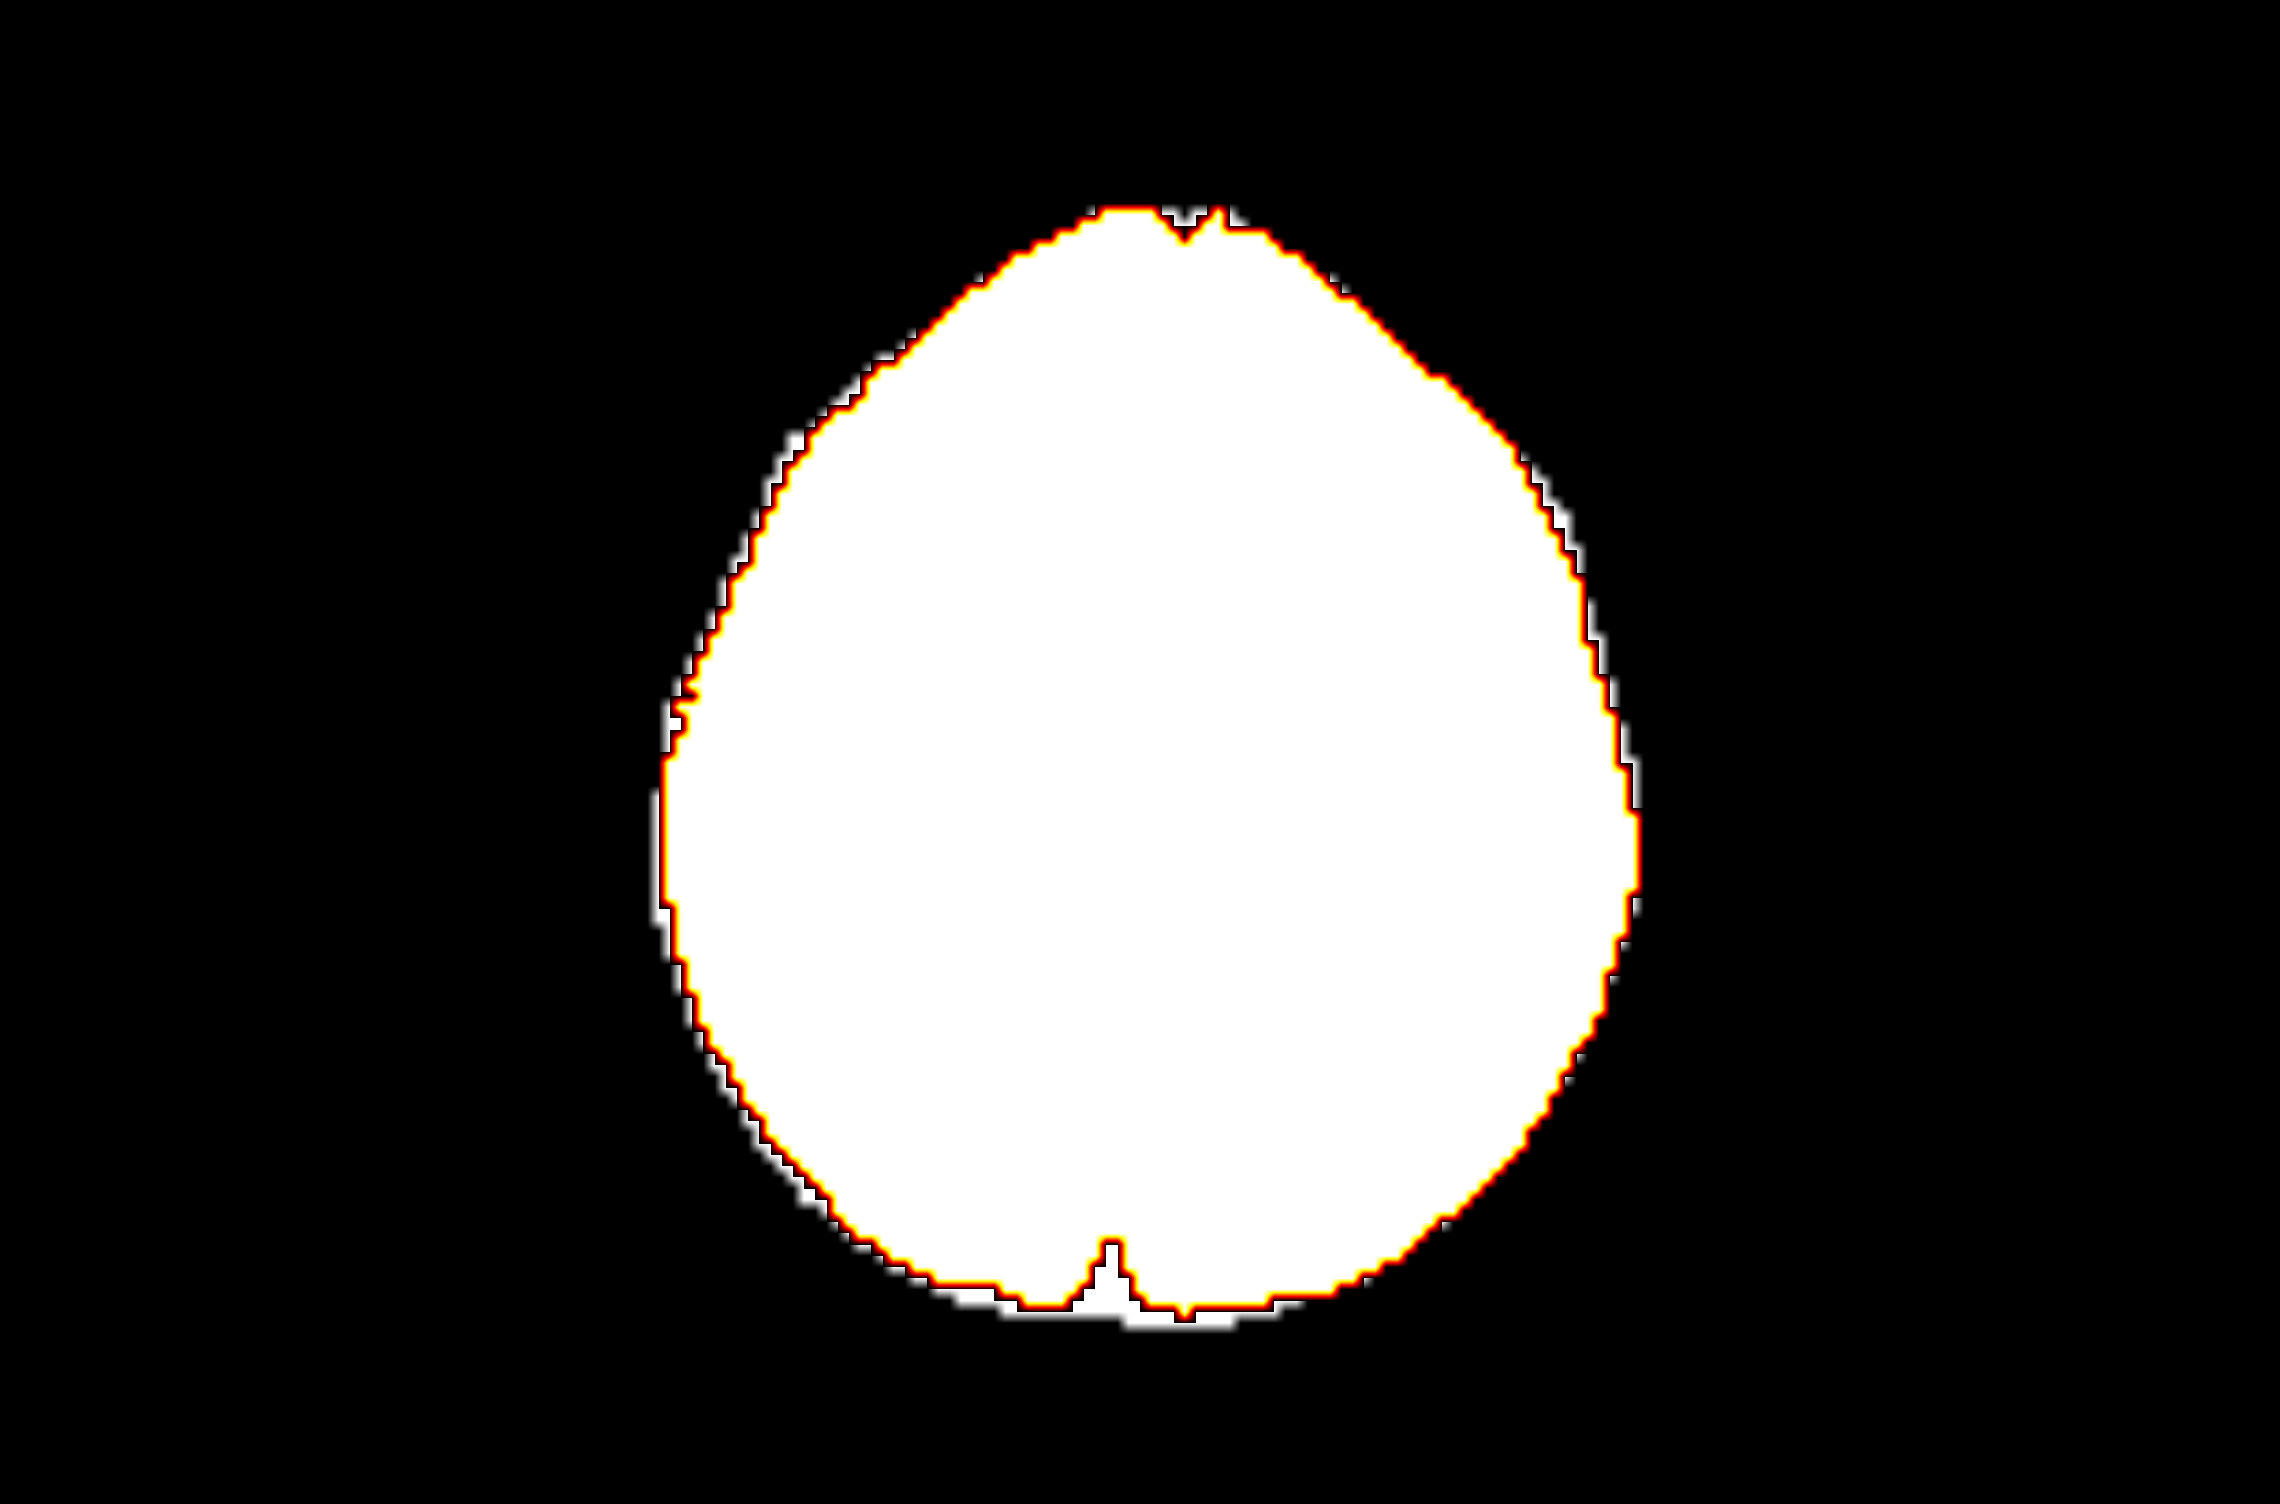
\includegraphics[width=0.6\textwidth]{Images/mask.png}}
  \caption{Example of the mask estimated using tissue volume fractions overlaid on the SynthStrip mask.}
  \label{fig:mask}
\end{figure}

\section{Analysis Pipeline}

The analysis was performed using MRtrix3 \cite{Tournier2019}. The main steps for the MT-CSD pipeline are outlined below:

\begin{enumerate}
    \item \textbf{Response Function Estimation:} Unsupervised estimation of response functions for WM, GM, and CSF was performed for each subject with \texttt{dwi2response} \cite{raffelt2019}. The estimated functions were then averaged across subjects to generate study-specific response functions for each tissue type.

    \item \textbf{MT-CSD:} Multi-tissue CSD was performed to compute WM ODFs with \texttt{dwi2fod}\cite{Jeurissen2014}.

    \item \textbf{Intensity Normalization:} \texttt{mtnormalise} was used on the ODFs to normalize them and correct for intensity bias \cite{Dhollander21}.

    \item \textbf{Template Creation:} A subset of 10 subjects per group was randomly selected for unbiased population template creation using \texttt{population\_template}. Initial alignment was performed using rigid and affine registration, followed by non-linear registration for final template optimization.

    \item \textbf{Registration to Template:} Subject ODFs were registered to the template using \texttt{mrregister}. This included affine and non-linear ODF-guided registration and reorientation \cite{Raffelt12}. The registration is symmetric, computing forward (subject~$\rightarrow$~template) and inverse (template~$\rightarrow$~subject) warps by aligning both images in a midway space.

    \item \textbf{Template Mask Generation:} The group analysis mask was defined as the intersection of all individual warped brain masks, obtained by taking the voxel-wise minimum across subjects.

    \item \textbf{Remove Cerebellum and Brainstem:} These regions were excluded to focus on the rest of the brain, thereby increasing statistical power by reducing the number of comparisons and speeding up the analysis.

    \item \textbf{Fixel Mask Generation:} ODFs were segmented in the template to create a fixel analysis mask using \texttt{fod2fixel}.

    \item \textbf{Warp Subject ODFs:} Each subject's ODFs were warped to the template space without reorientation using  \texttt{mrtransform}.

    \item \textbf{AFD Computation:} AFD values were computed by segmenting each subject's warped ODFs in the template space.

    \item \textbf{Fixel Reorientation:} Fixels were reoriented based on local angular transformations derived from the deformation fields at each voxel with \texttt{fixelreorient}.

    \item \textbf{Fixel Correspondence:} Fixels from each subject were matched to the template fixels using an angular threshold to identify the closest correspondence with minimal angular difference with \texttt{fixelcorrespondence}.

    \item \textbf{FC and FDC Computation:} Fixel-wise FC values were found from the Jacobian of the warp fields using \texttt{warp2metric}, log-transformed to ensure data are centred around zero and normally distributed, and multiplied by AFD to compute FDC.

    \item \textbf{Tractography and Smoothing:} A whole-brain tractogram was generated starting from the template, followed by the generation of the connectivity matrix and fixel-wise smoothing (\texttt{tckgen, fixelconnectivity, fixelfilter}).

    \item \textbf{Statistical Analysis:} Group-wise statistical comparisons were conducted using \texttt{fixelcfestats}, which implements a GLM and CFE, by defining appropriate design and contrast matrices.
\end{enumerate}

In the case of LoRE-SD, the pipeline does not include steps 1-3. The alternative steps are as follows:

\begin{enumerate}
    \item  \textbf{LoRE-SD: } LoRE-SD is applied to the diffusion data to obtain for each subject in each voxel a local response function and a unit-normalized ODF. The response function is described as a linear combination of Gaussian basis functions with corresponding weights (Gaussian fractions).

    \item \textbf{Contrasts Computation:} Contrast matrices are defined either assigning values to the grid of axial and radial diffusivities or by finding them through least squares from a pre-existing contrast. For each subject contrast images are obtained by taking the inner product of the contrast matrix with the Gaussian fractions found through LoRE-SD.

    \item \textbf{ODFs Scaling:} Unit-normalized ODFs found with LoRE-SD are scaled by performing a voxel-wise multiplication with the contrasts found in the previous step.

    \item \textbf{Cropping:} To completely exclude noisy ODFs from the analysis, images are cropped using brain masks, by multiplying the ODFs by the binary mask. This way, everything outside the brain is set to zero.
    
\end{enumerate}

\section{Contrast Computation in LoRE-SD}
Contrast matrices are defined by assigning weigths from 0 to 1 to the Gaussian basis functions parametrized by $\lambda_{\parallel}$ and $\lambda_{\perp}$.
Figure~\ref{fig:contrast} shows how the intra-axonal contrast is obtained in a 10 by 10 grid of basis functions. The contrast can be modified by adjusting the rate of the exponential decay of the weights with increasing $\lambda_{\perp}$, or by imposing anisotropy, meaning that all cells on the diagonal are set to 0, suppressing all isotropic basis functions.

Another contrast mimics the value of FA and it can be seen in Figure~\ref{fig:fa}. The equation of the FA metric from DTI (\ref{eq:FA}), with $\lambda_{\parallel}$ as $\lambda_{1}$ and $\lambda_{\perp}$ as $\lambda_{2}$ and $\lambda_{3}$, is used to assign a value to each combination of parameters.

\begin{figure}[h]
  \centering
  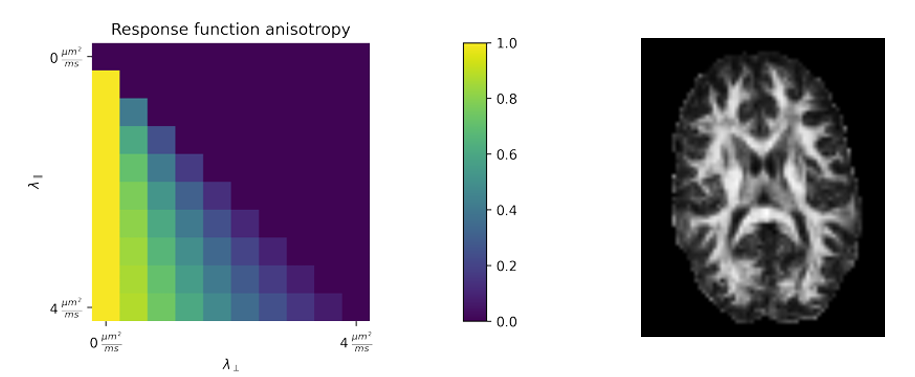
\includegraphics[width=0.7\textwidth]{Images/fa.png} % or use height= for vertical sizing
  \caption{Contrast matrix defining the FA contrast and resulting contrast for a subject.}
  \label{fig:fa}
\end{figure}
 

In theory, any contrast can be used to directly scale the ODFs. Another approach is to derive contrast matrices from existing contrast images by solving an optimization problem. A least-squares optimization can be used to determine the combination of basis functions (contrast matrix) that best reproduces the input contrast when applied to the Gaussian fractions from LoRE-SD. The problem can be written as a constrained linear least square problem:

\begin{align}
\min_{\boldsymbol{x}} \quad & \frac{1}{2} \left\| A \boldsymbol{x} - \boldsymbol{b} \right\|^2 \\
\text{subject to} \quad & \boldsymbol{0} \leq \boldsymbol{x} \leq \boldsymbol{1}
\end{align}
Here, $A$ contains the input Gaussian fractions that define the local response function in each voxel, b is the target image contrast assigning a value to each voxel, and $\boldsymbol{x}$ represents the weights for each Gaussian basis function (each point on the grid). We impose that the weights have to be between 0 and 1. The optimization problem was solved using the \texttt{lsq\_linear} function from the SciPy library \cite{Virtanen2020}.
Solving this provides a data-driven contrast matrix that emphasizes the contribution of the tissue compartments underlying the given image contrast. This approach not only provides a means to scale the ODFs, but also offers insight into the characteristics of the contrast.
\\A possible meaningful contrast to replicate is the WM volume fractions estimated from MT-CSD. Specifically, the first SH coefficient of the WM ODF can be used as the target contrast $\boldsymbol{b}$.

\section{Removal of Cerebellum and Brainstem}
To improve statistical power and reduce computational load, the cerebellum and brainstem were excluded from the FBA. The segmentation was performed using the T1-weighted anatomical images of the subjects, following these steps:

\begin{enumerate}
    \item \textbf{Rigid Registration:} The average $b=0$ diffusion image was rigidly registered to the subject's T1-weighted image. Rigid registration is used because the images belong to the same subject so the difference won't be in the anatomy but only due to the patient moving or different positioning. 

    \item \textbf{Transform T1 to DWI Space:} The inverse of the above transformation was applied to bring the T1-weighted image into diffusion space.

    \item \textbf{Transform to Template Space:} The subject-specific non-linear warp (obtained during registration to the group template) was then used to bring the T1 image from diffusion space to template space.

    \item \textbf{Segmentation of Cerebellum and Brainstem:} SynthSeg \cite{billot2023} was used to segment the cerebellum and brainstem from the T1-weigted image in template space. SynthSeg is a deep learning-based tool that uses CNNs trained entirely on synthetic data, enabling robust segmentation without the need for retraining or fine-tuning. This resulted in a binary mask for each subject that excludes the cerebellum and brainstem.

    \item \textbf{Mask Averaging:} The individual binary masks were averaged across subjects. Voxels with an average value below 0.5 were set to 0, removing only voxels consistently excluded across subjects.

    \item \textbf{Resolution Adjustment:} The resulting mask, originally at T1 resolution, was downsampled to match the resolution of the diffusion data.

    \item \textbf{Combination with Template Mask:} The cerebellum-brainstem exclusion mask was combined with the main template mask using a voxel-wise minimum (logical AND), ensuring that only voxels common to all subjects and excluding unwanted regions were included in the analysis.

    \item \textbf{Fixel Mask Creation:} The final voxel-wise mask was converted to a fixel-wise mask by assigning a value of 0 to all fixels in voxels with value 0, and 1 to the rest using MRtrix3 command \texttt{voxel2fixel} \cite{Tournier2019}. This fixel mask was used to define the region of interest in the statistical analysis.
\end{enumerate}

\section{Fixels Extraction}
\label{sec:extract}

\begin{table}[H]
    \caption*{\textbf{Number of fixels obtained by changing the threshold for different ODF templates}} % bold visible title
    \centering 
    \begin{tabular}{|l c c|}
    \hline
    \rowcolor{bluepoli!40}
    \textbf{ODF Template} & \textbf{Threshold} & \textbf{Number of fixels} \T\B \\
    \hline \hline
    MT-CSD & 0.06 & 365585 \T\B \\
    LoRE-SD with intra-axonal scaling & 0.06 & 379857 \T\B \\
    LoRE-SD with intra-axonal scaling & 0.07 & 327759 \T\B \\
    LoRE-SD with FA scaling & 0.06 & 455263 \T\B \\
    LoRE-SD with FA scaling & 0.07 & 379065 \T\B \\
    LoRE-SD with FA scaling & 0.08 & 323570 \B \\
    \hline
    \end{tabular}
    \\[10pt]
    \caption{Number of fixels obtained by changing the threshold value on the lobe amplitude for different ODF templates.}
    \label{tab:fixels}
\end{table}


To derive fixels from both the template and subject ODFs, a threshold on the lobe amplitude must be defined. This threshold determines which peaks in the ODFs are segmented as fixels. It is important to extract a sufficiently large number of fixels and to ensure that fixels are present also in regions with crossing fibres. The optimal threshold may vary based on the data and the preprocessing steps. Also it can depend on whether MT-CSD or LoRE-SD is used, and for the latter also on which contrast was used for scaling. The thresholds and the resulting numbers of fixels can be found in \cref{tab:fixels}. 

Figure~\ref{fig:fixels} shows some details of the extracted fixels.

\begin{figure}[H]
  \centering
  \subfloat[MT-CSD ($\tau = 0.06$)\label{fig:mtcsd}]{
    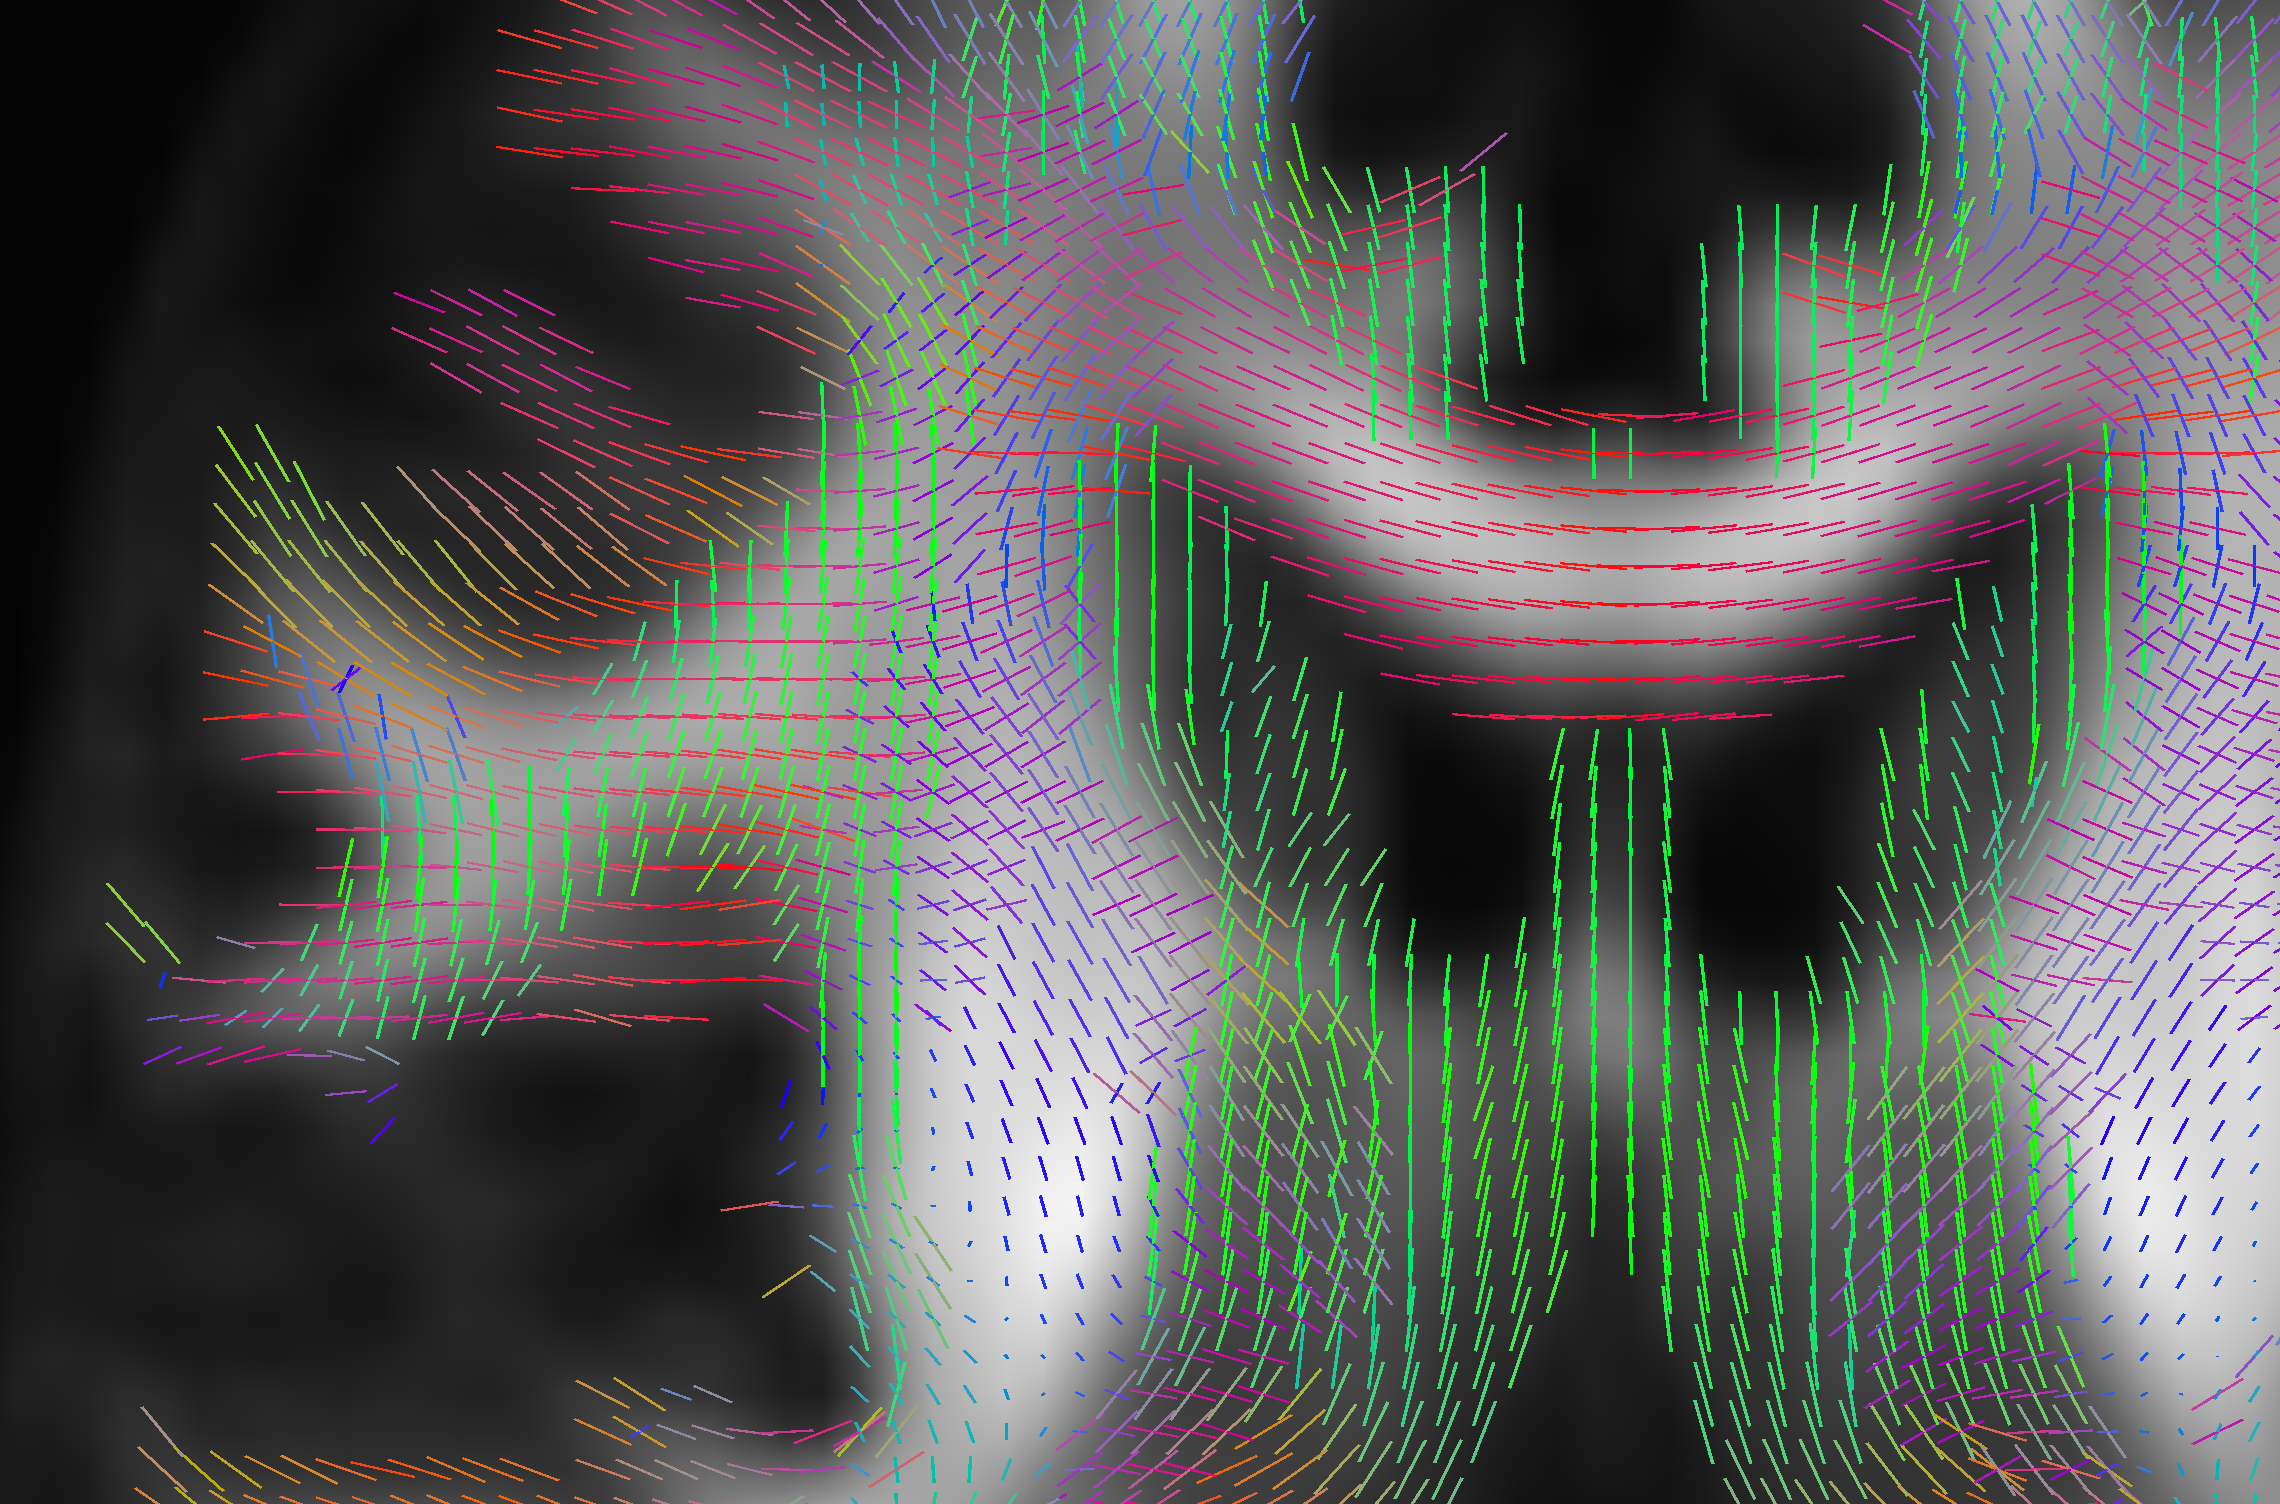
\includegraphics[width=0.45\textwidth]{Images/comparison_MTCSD0005.jpg}
  }
  \hfill
  \subfloat[LoRE-SD (intra-axonal, $\tau = 0.06$)\label{fig:lore06}]{
    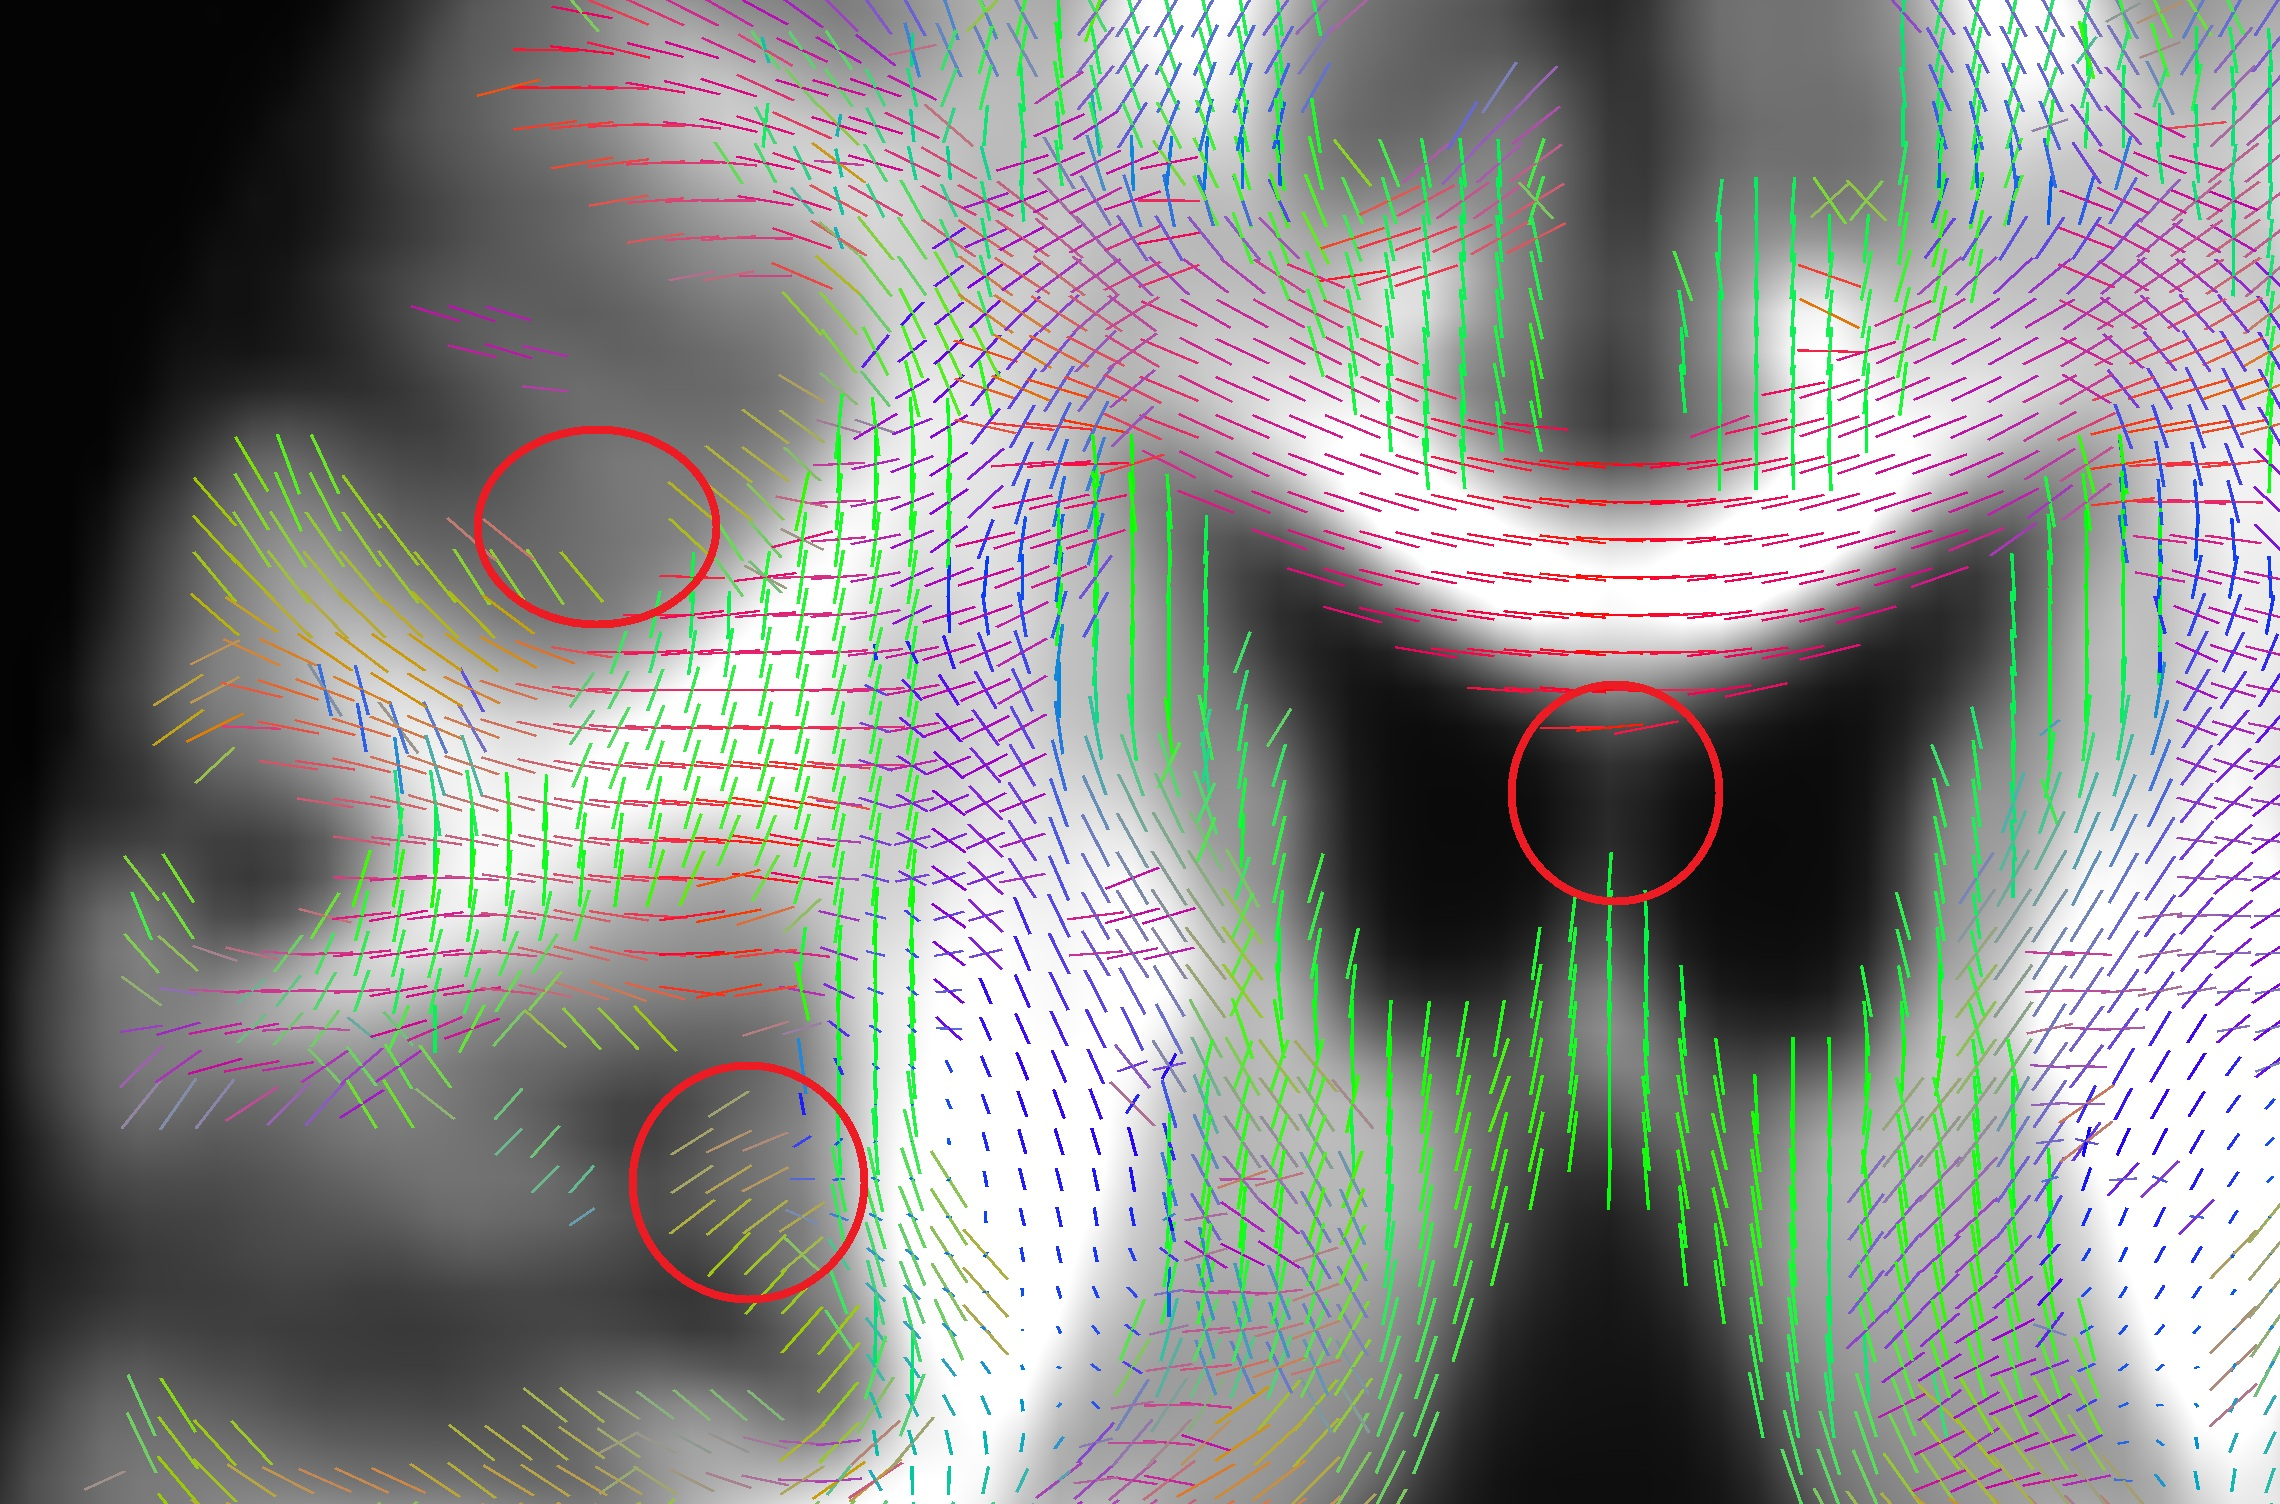
\includegraphics[width=0.45\textwidth]{Images/comparison_intra_axona_annotated.jpg}
  }
  \hfill
  \subfloat[LoRE-SD (intra-axonal, $\tau = 0.07$)\label{fig:lore07}]{
    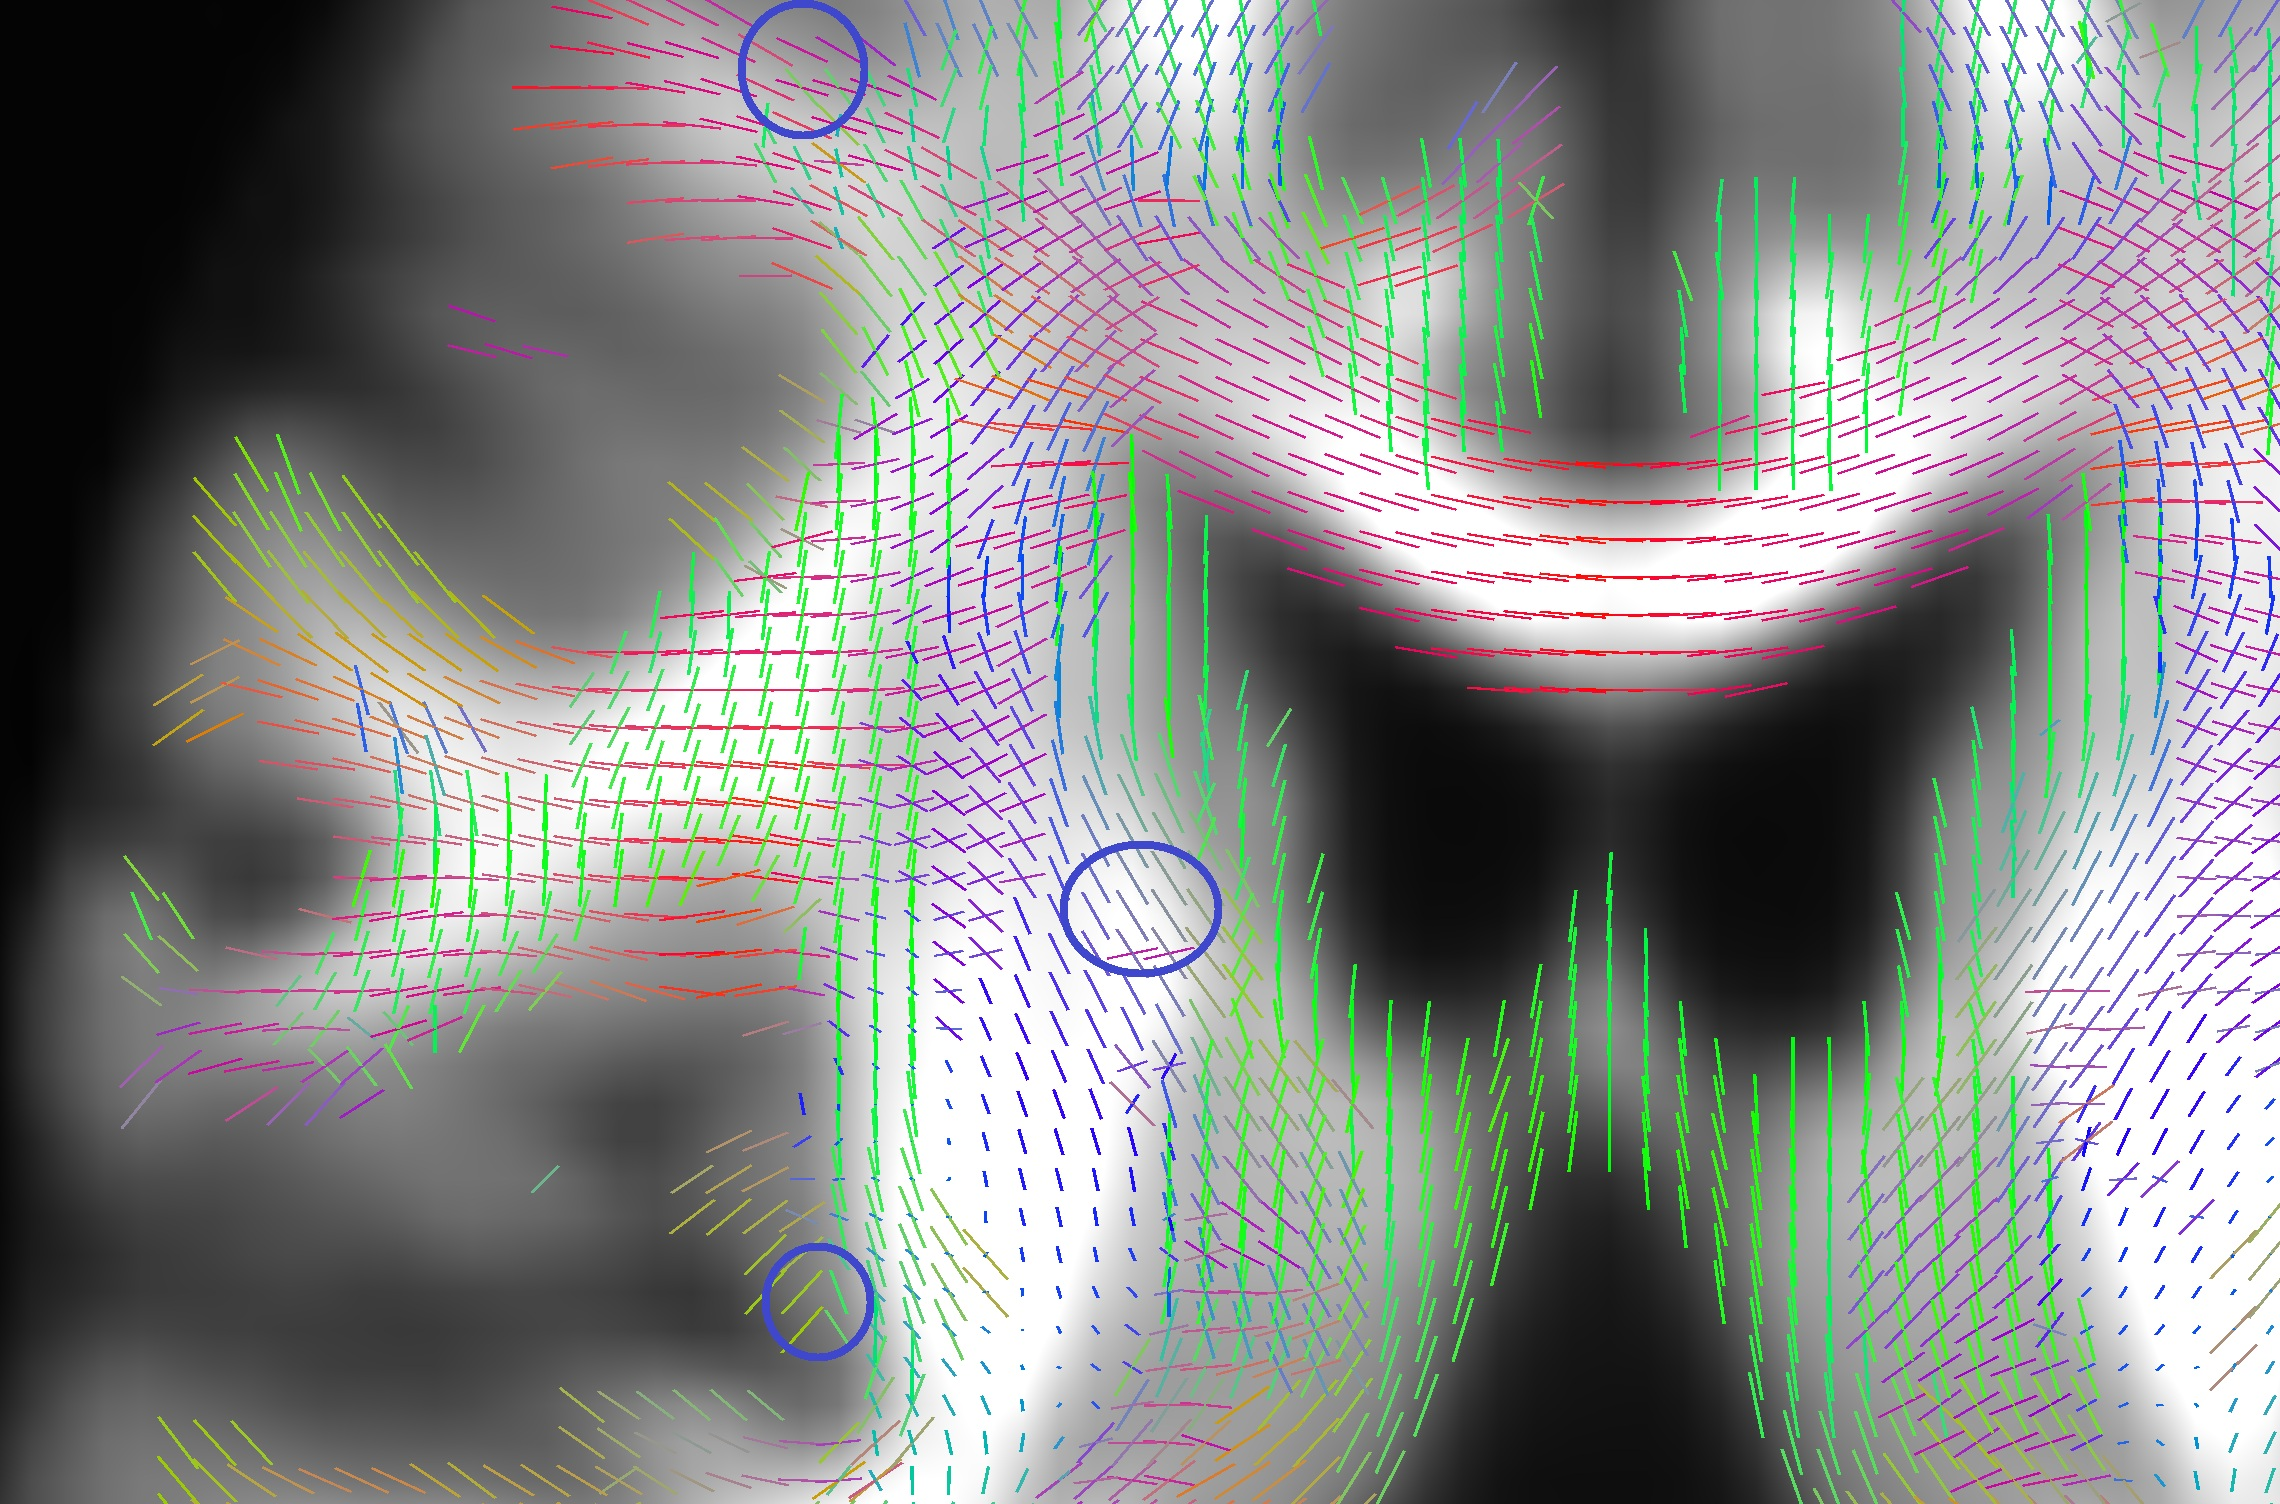
\includegraphics[width=0.45\textwidth]{Images/comparison_intra_axonal_less_annotated.jpg}
  }
  \caption[Fixel masks]{Fixel masks for the first 3 cases reported in \cref{tab:fixels}. $\tau$ indicates the threshold on the lobe amplitude of the ODFs. Red circles show regions where MT-CSD and LoRE-SD differ. Blue circles show regions where fixels are lost when increasing the threshold.}
  \label{fig:fixels}
\end{figure}



It can be noted that there are some differences in the fixels extracted with the two methods. With the same threshold LoRE-SD results in a higher number of fixels, but increasing the threshold could lead to the loss of some important fixels. Figure~\ref{fig:fixels} shows that increasing the threshold leads to the loss of some fixels in crossing fiber regions. For this reason the lower threshold was chosen for the intra-axonal contrast. For the FA contrast 0.07 seems to be a better choice.


\section{Tractography}
The tractography algorithm employed was iFOD2 \cite{Tournier2010}, a probabilistic method that starts from the information contained in the ODFs. The algorithm favors tracking along directions with higher ODF amplitudes, while still allowing propagation through lower-amplitude directions as long as values are higher than a given threshold. iFOD2 generates streamlines by propagating along short arcs tangent to the current direction, which improves anatomical plausibility. Tracking was seeded randomly within the brain mask. The minimum ODF amplitude required to continue tracking was set to 0.06, only streamlines between 10 mm and 250 mm in length were accepted, and the maximum change in underlying fibre orientation between the start and end points of each step was set to 22.5$^\circ$. This last parameter controls the smoothness of the resulting streamlines \cite{Smith2012}. A total of 20 million streamlines were generated.

To reduce biases in tractogram density and improve biological plausibility, SIFT (Spherical-deconvolution Informed Filtering of Tractograms) was applied \cite{Smith2013}. This method refines the tractogram by iteratively removing streamlines (from 20 to 2 million in our case) to only keep the ones that best match the underlying ODFs. SIFT works by comparing the density of streamlines in each voxel with the integral of the ODF lobes in corresponding directions. The assumption is that larger ODF lobes represent regions with more axons oriented in that direction, and so with a higher density of streamlines.

\begin{figure}[h]
  \centering
  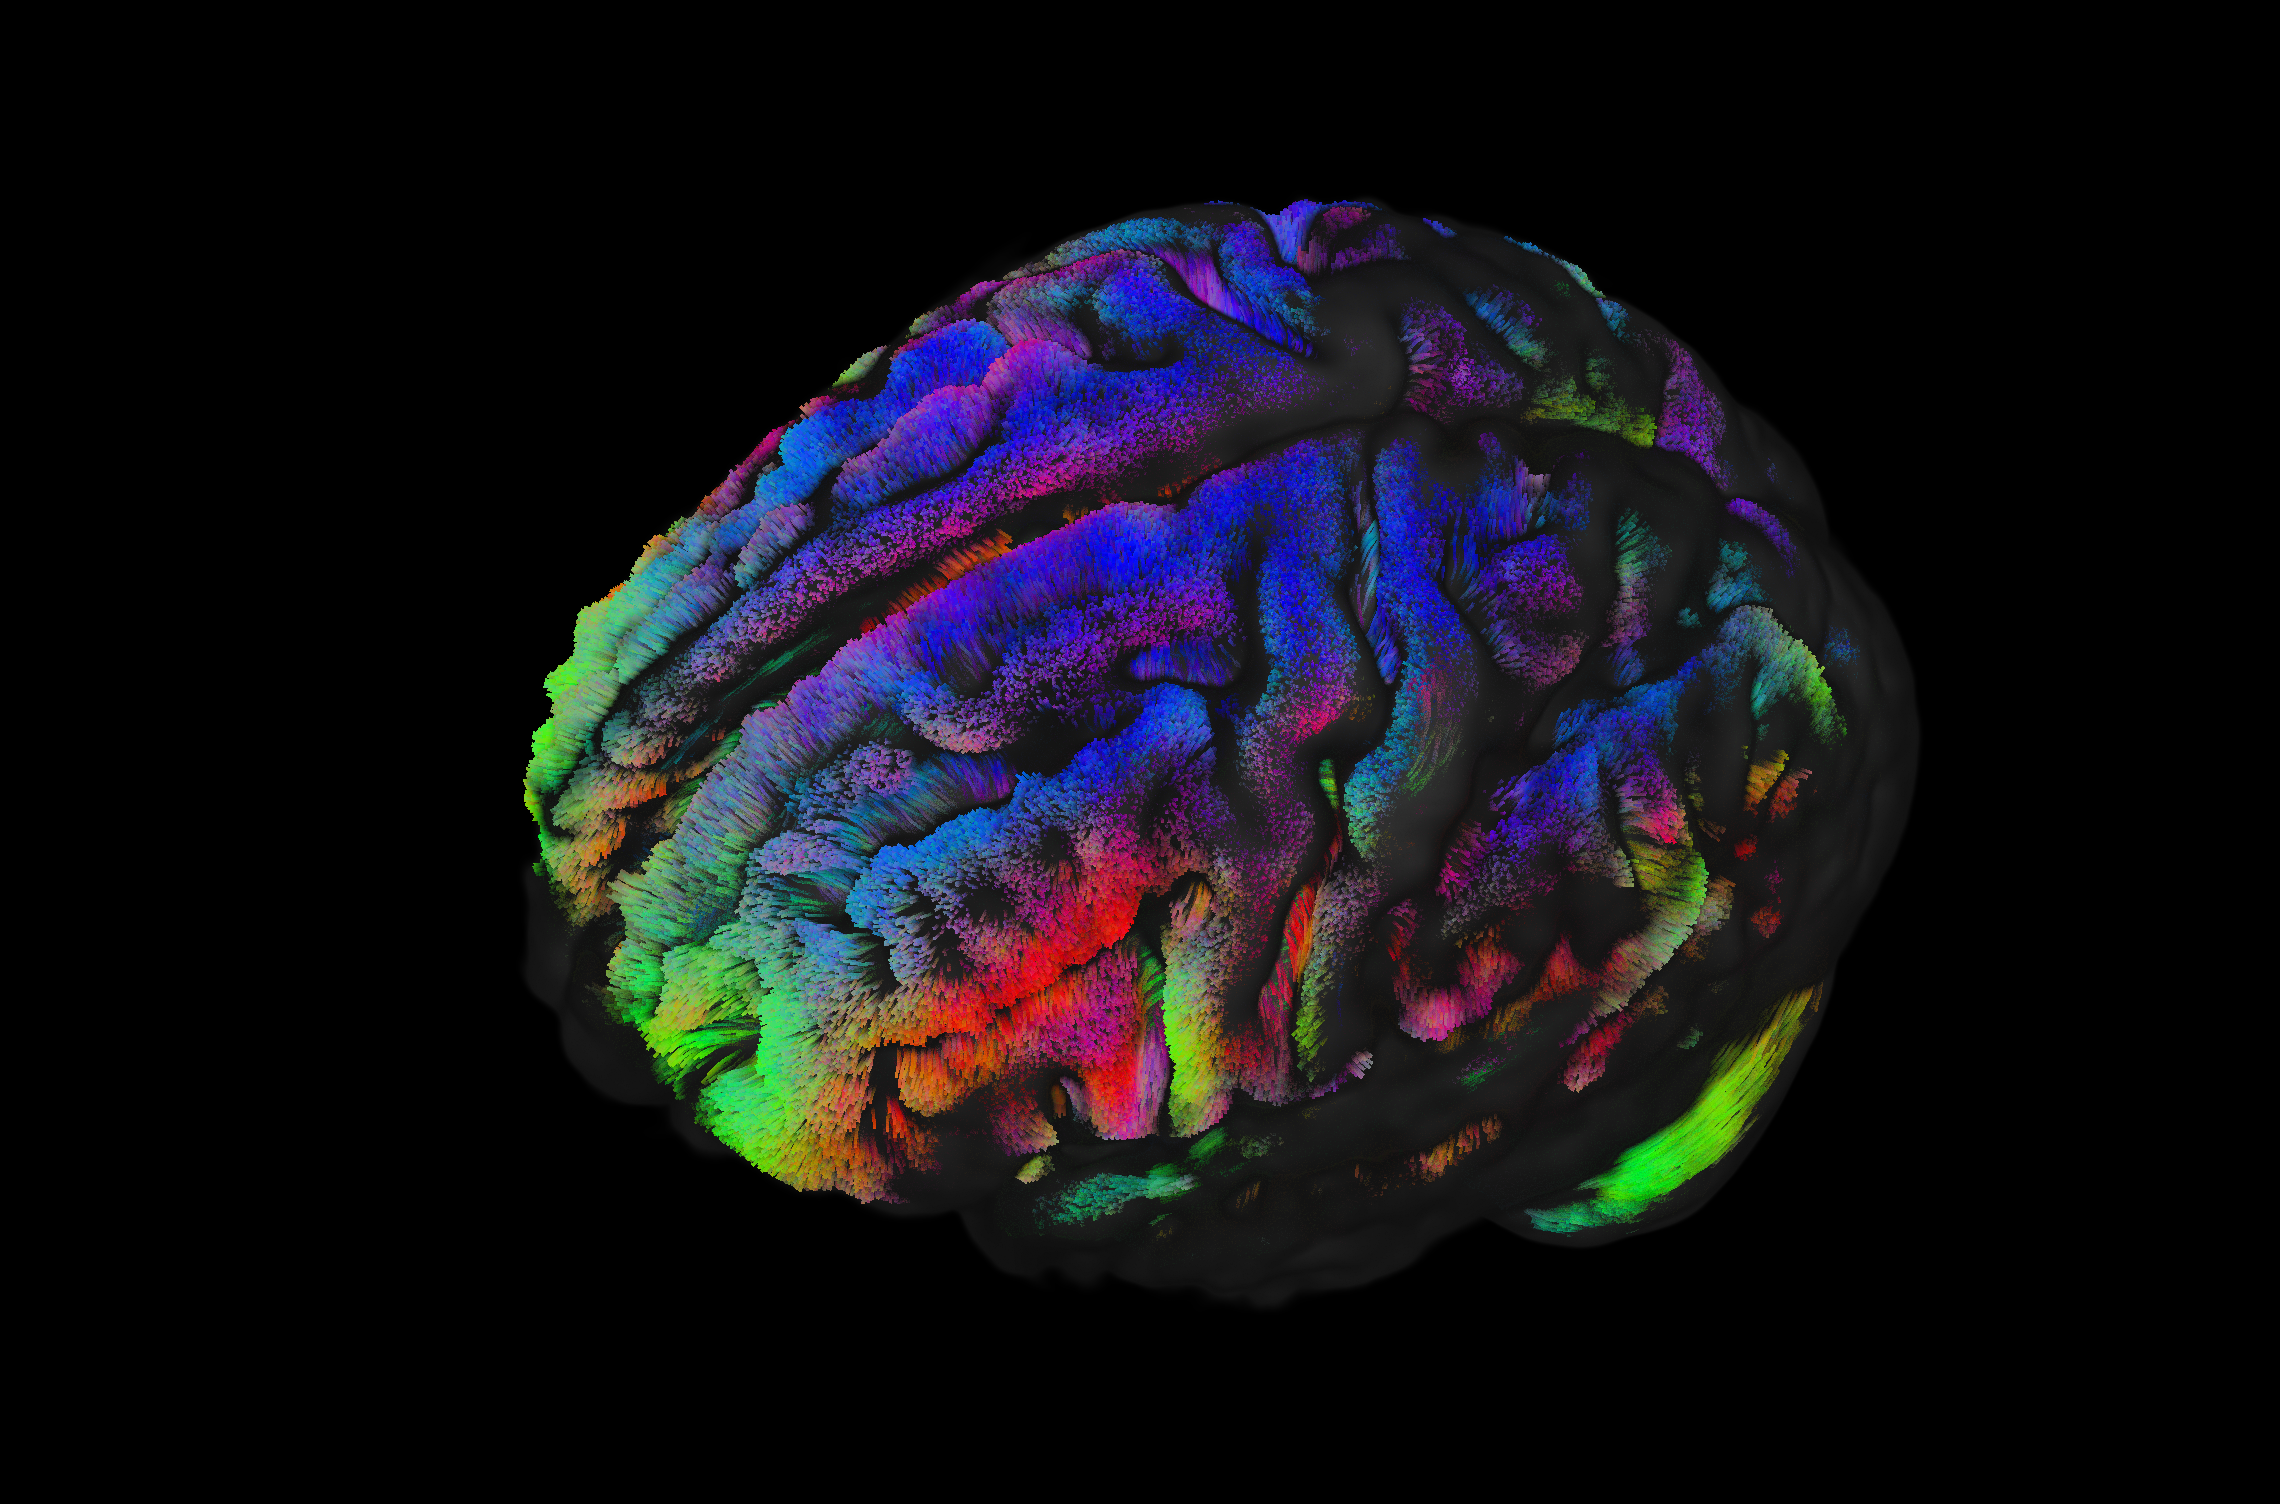
\includegraphics[width=0.5\textwidth]{Images/tractography.png} % or use height= for vertical sizing
  \caption{Tractography of the template obtained using the results of MT-CSD.}
  \label{fig:tractography}
\end{figure}

\section{Statistical Analysis}
For FBA, we can formulate the statistical analysis as a GLM which has the form \cite{Winkler2014}:
\begin{equation}
{Y} = {M} \boldsymbol{\psi} + \boldsymbol{\epsilon}
\end{equation}
where ${Y}$ is the observed data, ${M}$ the design matrix, $\boldsymbol{\psi}$ contains the regression coefficients estimated using least squares, and $\boldsymbol{\epsilon}$ the random errors.
We can split ${M}$ in the following way:
\begin{equation}
{Y} = {X} \boldsymbol{\beta} + {Z} \boldsymbol{\gamma} + \boldsymbol{\epsilon}
\end{equation}
where ${X}$ contains the regressors of interest and ${Z}$ the nuissance regressors (covariates).

In our case ${Y}$ is the values of a certain metric (e.g., AFD) for a specific fixel across all subject in the study. So, it will have dimension of 101x1. Since we want to compare the different groups, ${X}$ contains one column per group (CP, CM, HC), resulting in dimensions 101x3, with a 1 indicating group membership and 0 otherwise. ${Z}$ contains a column for the age and one for the intracranial volume (ICV) when relevant. ICV can play a role when analyzing FC and FDC, as they contain information regarding volume changes. Both age and ICV need to be normalized. In this model, the values of the vector $\boldsymbol{\beta}$ ($\beta_1$, $\beta_2$, $\beta_3$) represent the mean metric value for each group when the covariates are 0 (at mean age and ICV). The coefficients of $\boldsymbol{\gamma}$ reflect the effect of the covariates.

To formally test hypotheses about group differences, a contrast matrix $\mathbf{C}$ is defined. For a one-sided directional test, the null hypothesis is written as \cite{Winkler2014}:

\begin{equation}
H_0: {C}\boldsymbol{\psi} \leq 0
\end{equation}

${C}$ defines a linear combination of model parameters. In our case we are interested in testing differences in the mean values between groups. For example, ${C} = [-1 \; 0 \; 1 \; 0 \; 0]$ tests whether $\beta_3 > \beta_1$, i.e., whether the metric is higher in healthy controls (HC) than in chemo-treated patients (CP) for a given fixel. Since the interpretability of the fixel-wise metrics may not always be straightforward, both directions need to be tested (e.g., $\beta_3 > \beta_1$ and $\beta_1 > \beta_3$).
\\In the analysis,  the pairwise difference in both directions between groups for all metrics will be tested and significance will be determined as described in the previous chapter, using permutation testing and CFE.

\section{Statistical Power and Track Density Imaging}
Given the large number of fixels (on the order of 300,000), and so of statistical tests, corrections for multiple comparisons can become so stringent that detecting meaningful effects is extremely difficult. 
One common approach to partially solve this problem is to reduce the number of tests by focusing on specific regions of interest \cite{Cremers2017, Lindquist2015}. 
For example, prior knowledge about which brain regions are related to the disease of interest can guide the selection of relevant tracts, as demonstrated in the context of FBA by Mito et al.\ \cite{Mito2018}.
Another way to enhance statistical power, without the need to choose a region of interest (ROI) a priori, is through tract density imaging (TDI) \cite{Calamante2010}. This technique uses the results of tractography to generate an image in which voxel intensity reflects the number of streamlines passing through each voxel. This can be extended to fixels by assigning to each one the number of streamlines passing through it. Then, we can apply a threshold to generate a fixel mask, excluding from the analysis fixels with low streamline density, which are likely to be poorly connected to the rest of the brain. This allows to focus on more meaningful regions and improve the chances of detecting significant effects.

\chapter{Results}
In this chapter, we present results in two parts. First, we show ODF templates and evaluate contrast scaling strategies for LoRE-SD. Second, we report group comparisons of fixel-wise metrics (AFD, FC, FDC) across CP, CM, and HC groups, using both MT-CSD and LoRE-SD. Key findings include increased AFD in the CP group compared to HC, particularly in the fornix and regions near the ventricles. Finally, we show that using a reduced fixel mask increases the number of significant fixels in these areas.

\section{Templates}

\begin{figure}[h!]
  \centering
  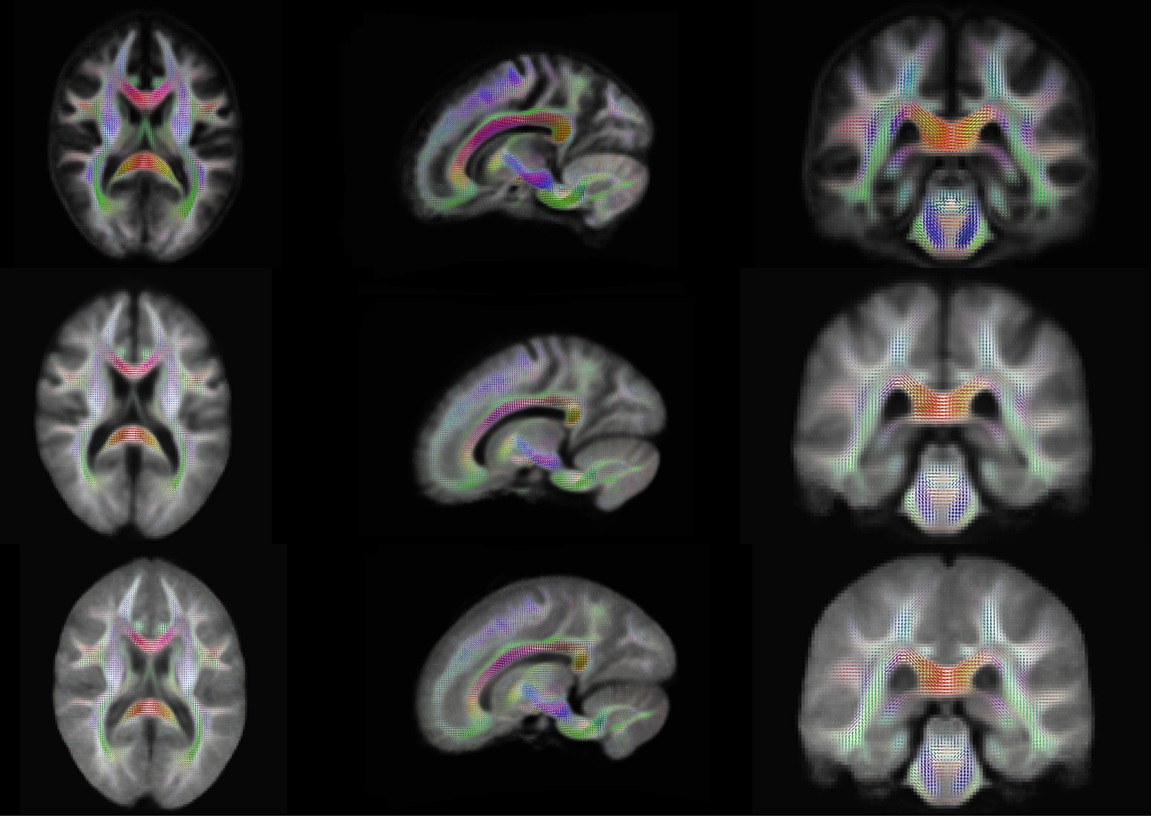
\includegraphics[width=0.8\textwidth]{Images/template_new.jpg} % or use height= for vertical sizing
  \caption{The three ODF templates used in the analysis. Top: WM ODF from MT-CSD. Middle: LoRE-SD ODF scaled with intra-axonal contrast. Bottom: LoRE-SD ODF scaled with FA contrast. ODFs are directionally colored and overlaid on a grayscale image of the first SH coefficient.}
  \label{fig:template_odf}
\end{figure}

Three ODF templates were generated and used as the basis for the subsequent analysis. An example illustrating their differences is shown in Figure~\ref{fig:template_odf}. 
\\The intra-axonal template was used as the reference space also for ODFs scaled with different contrasts (WM, FA, and anisotropic intra-axonal).


\section{LoRE-SD scaling contrasts}
\label{sec:cont}

\begin{figure}[H]
    \centering
    \subfloat[Contrast matrices.\label{fig:subfig-cont}]{
        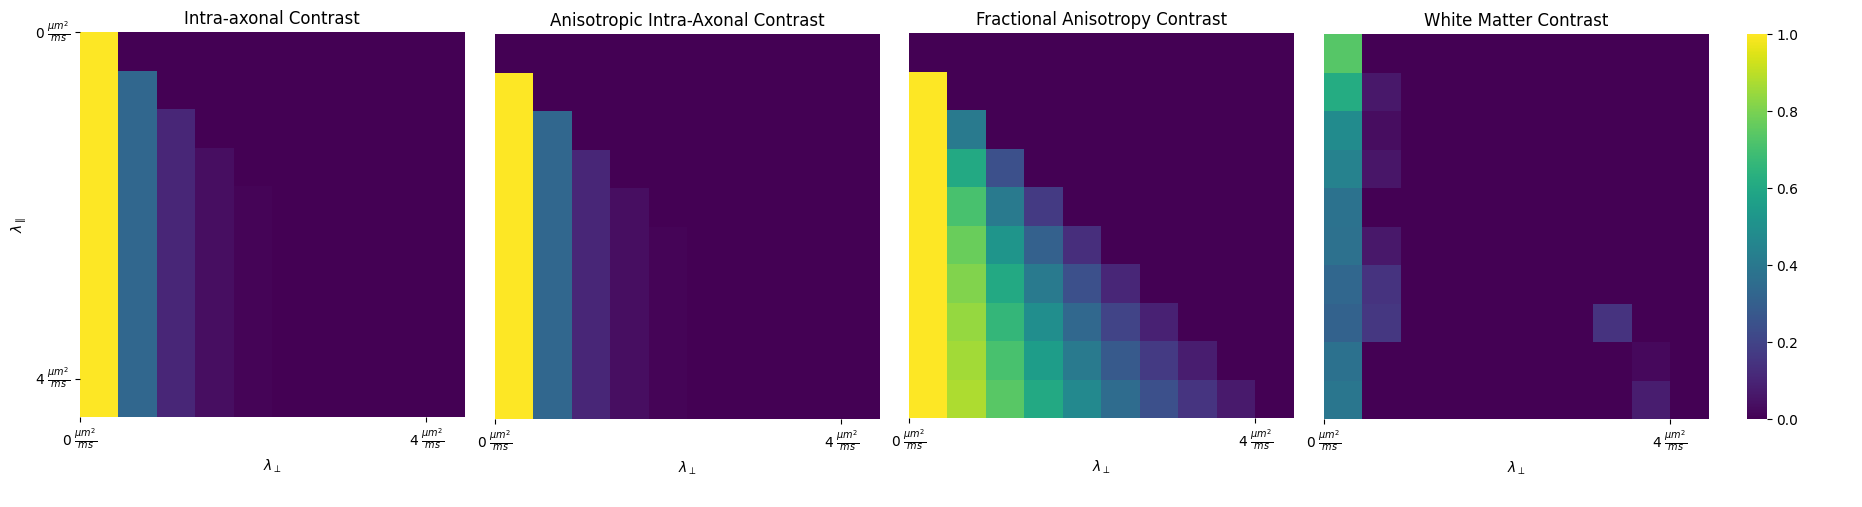
\includegraphics[width=
        \linewidth]{Images/contrast_combined.jpg}
    } \\ % <-- line break forces stacking
    \subfloat[Corresponding contrasts.\label{fig:subfig-other}]{
        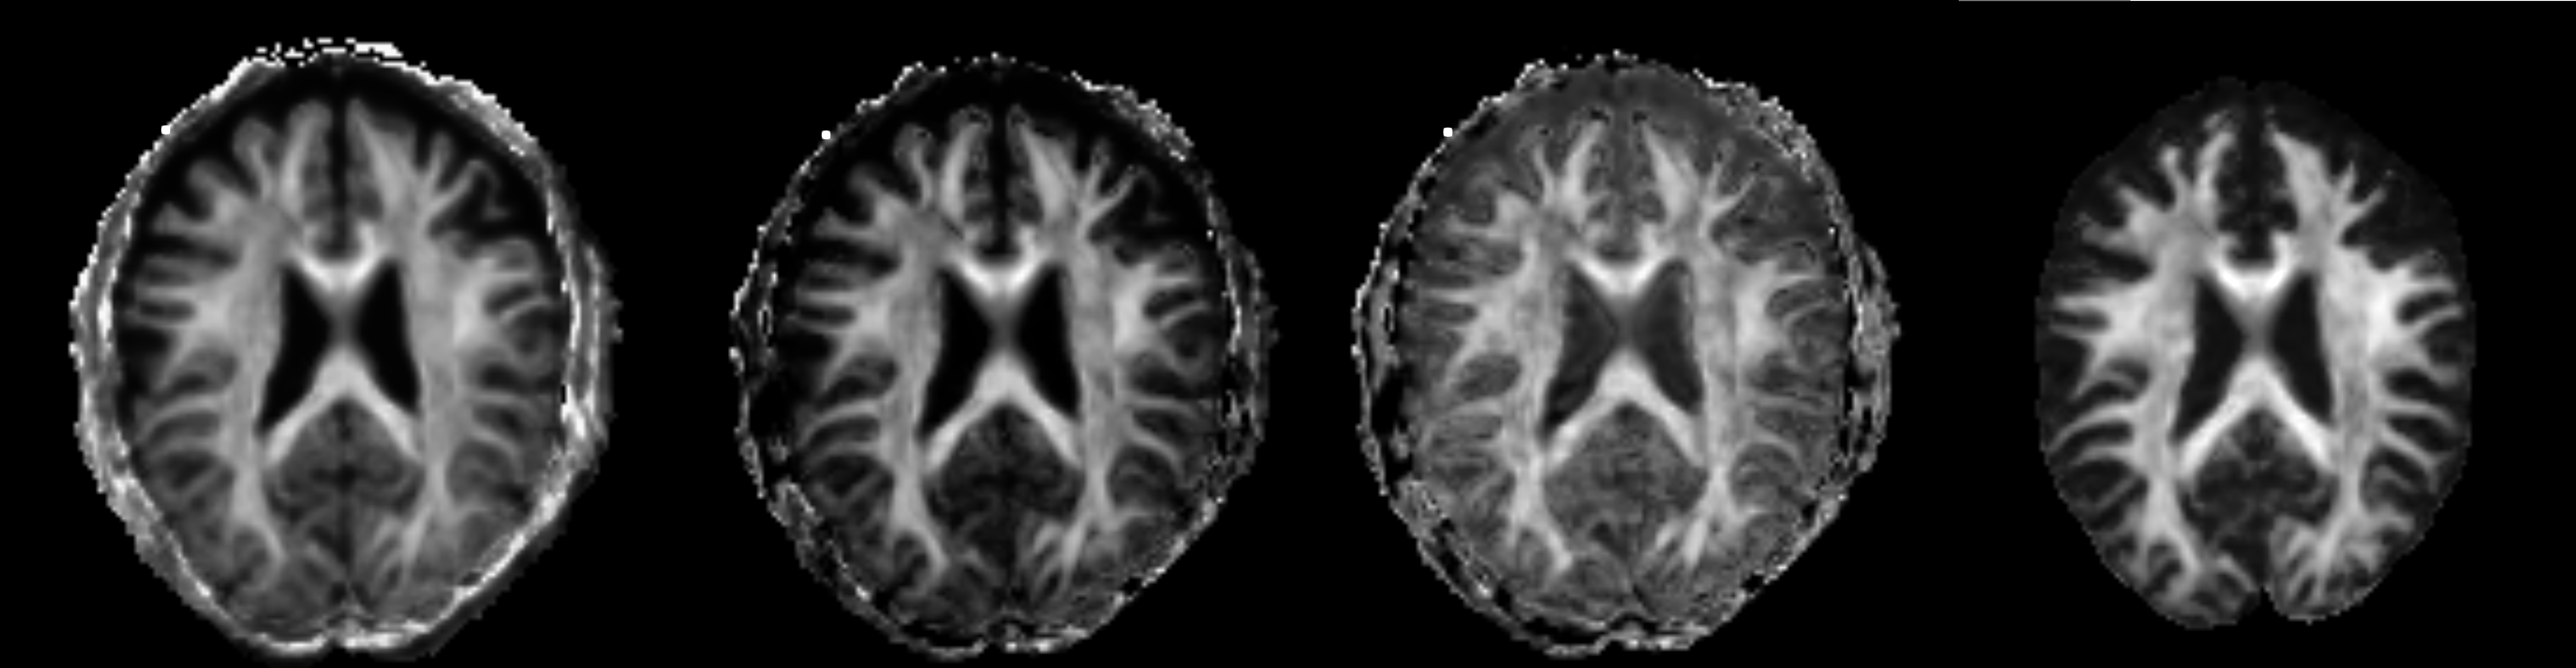
\includegraphics[width=0.8\linewidth]{Images/combined2.jpg}
    }
    \caption{Contrast matrices assigning a weight to each Gaussian basis function (a) and corresponding scaling contrasts (b) for one CP subject.}
    \label{fig:contrast_combined}
\end{figure}



Figure~\ref{fig:contrast_combined} shows all the contrast matrices and the corresponding contrasts which were used for scaling the ODFs. The fourth contrast matrix (white matter contrast) was derived for each subject by solving a constrained least squares optimization problem, aiming to find the matrix that produces a contrast best resembling the WM volume fractions obtained via MT-CSD.\\
Figure~\ref{fig:CM_10} shows the results for another subject from the CM group: the optimized contrast matrix, the resulting contrast, and the original input contrast.

For the intra-axonal contrast, making it anisotropic by setting all diagonal basis functions to zero (second matrix in ~\ref{fig:subfig-cont}) results in slightly smaller ODF amplitudes, particularly at tissue interfaces (Figure~\ref{fig:aniso}). As a consequence, fewer fixels are obtained.

\begin{figure}[h]
    \centering
    \subfloat[Contrast matrix obtained for a CM subject through optimization starting from the WM volume fractions.\label{fig:subfig-CM10}]{
        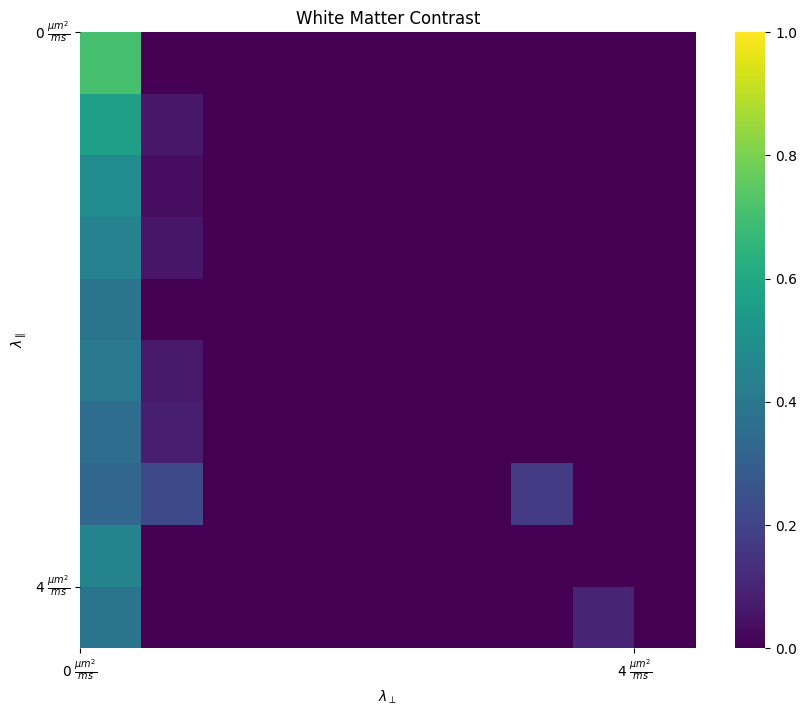
\includegraphics[width=0.5\linewidth]{Images/wm_matrix_CM_10.jpg}
    } \\[1em] % line break + vertical space
    \subfloat[Contrast obtained using the weights in a (left) and original contrast (right).\label{fig:subfig-b}]{
        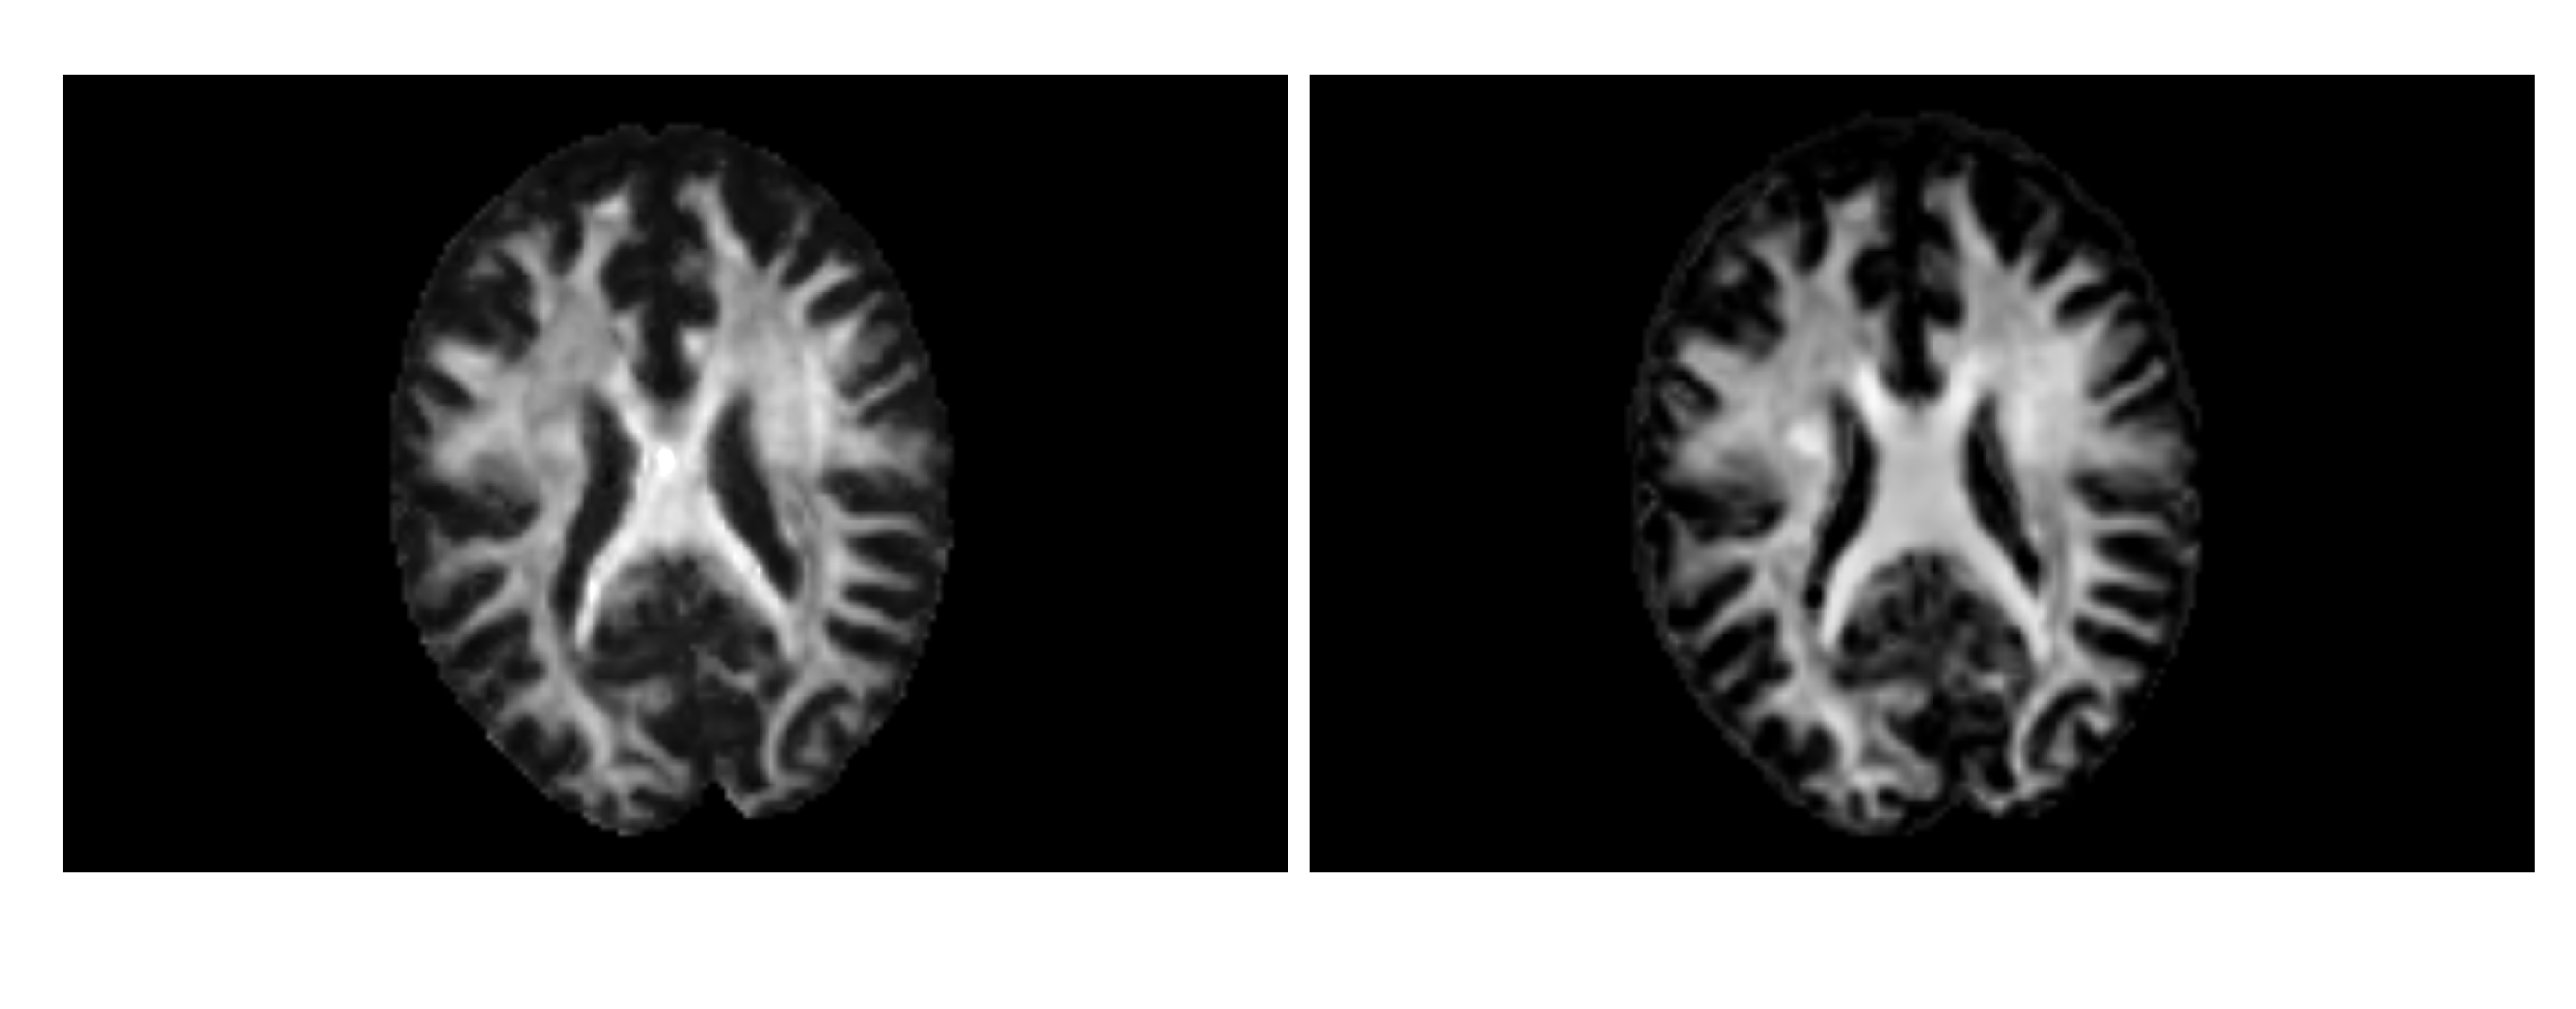
\includegraphics[width=\linewidth]{Images/CM_10.jpg}
    }
    \caption{WM contrast for a CM subject.}
    \label{fig:CM_10}
\end{figure}




\begin{figure}[H]
  \centering
  \includegraphics[width=0.9\textwidth]{Images/aniso.jpg} % or use height= for vertical sizing
  \caption{ODFs scaled with the intra-axonal contrast (left) and with the anisotropic intra-axonal contrast (right). ODFs are overlaid on a grayscale image representing the first SH coefficient.  The results are different mostly at tissue interfaces.}
  \label{fig:aniso}
\end{figure}

\section{Chemobrain}
Statistical tests were conducted to investigate differences among the CP, CM, and HC groups for the three fixel-wise metrics (AFD, log-FC, FDC), initially analyzing the whole brain excluding only the brainstem and cerebellum. Significant regions were identified as those containing fixels with a FWE-corrected p-value below 5\%. In this section, figures displaying results show fixels overlaid on grayscale images representing the first SH coefficient of the corresponding ODF template. This way anatomical context is provided. 

\subsection{MSMT-CSD}
Significant results were found for AFD when testing for a higher value in the CP group compared to HC. We found 637 significant fixels. No significant differences were found in any case for FDC and FC. 
\\AFD was significantly higher for fixels belonging to the fornix (Figure~\ref{fig:fornix1} and \ref{fig:fornix2}), but also in regions at the interface with the ventricles (Figure~\ref{fig:inter}) and in crossing fibre regions (Figure~\ref{fig:cross}).

\begin{figure}[h]
  \centering
  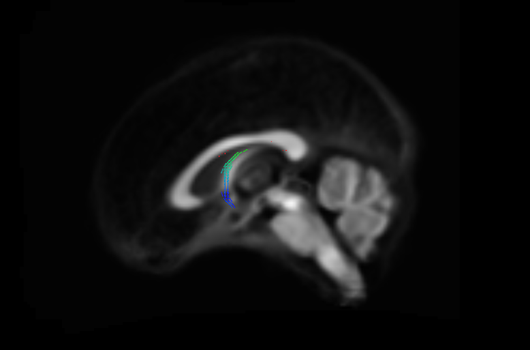
\includegraphics[width=0.9\textwidth]{Images/fornix1.jpg} % or use height= for vertical sizing
  \caption{Fixels derived with MT-CSD. Significant fixels found when testing a higher AFD in CP compared to HC. Significant fixels are colored based on their direction. The sagittal slice clearly shows the fornix as a region with significant AFD increase.}
  \label{fig:fornix1}
\end{figure}

\begin{figure}[H]
  \centering
  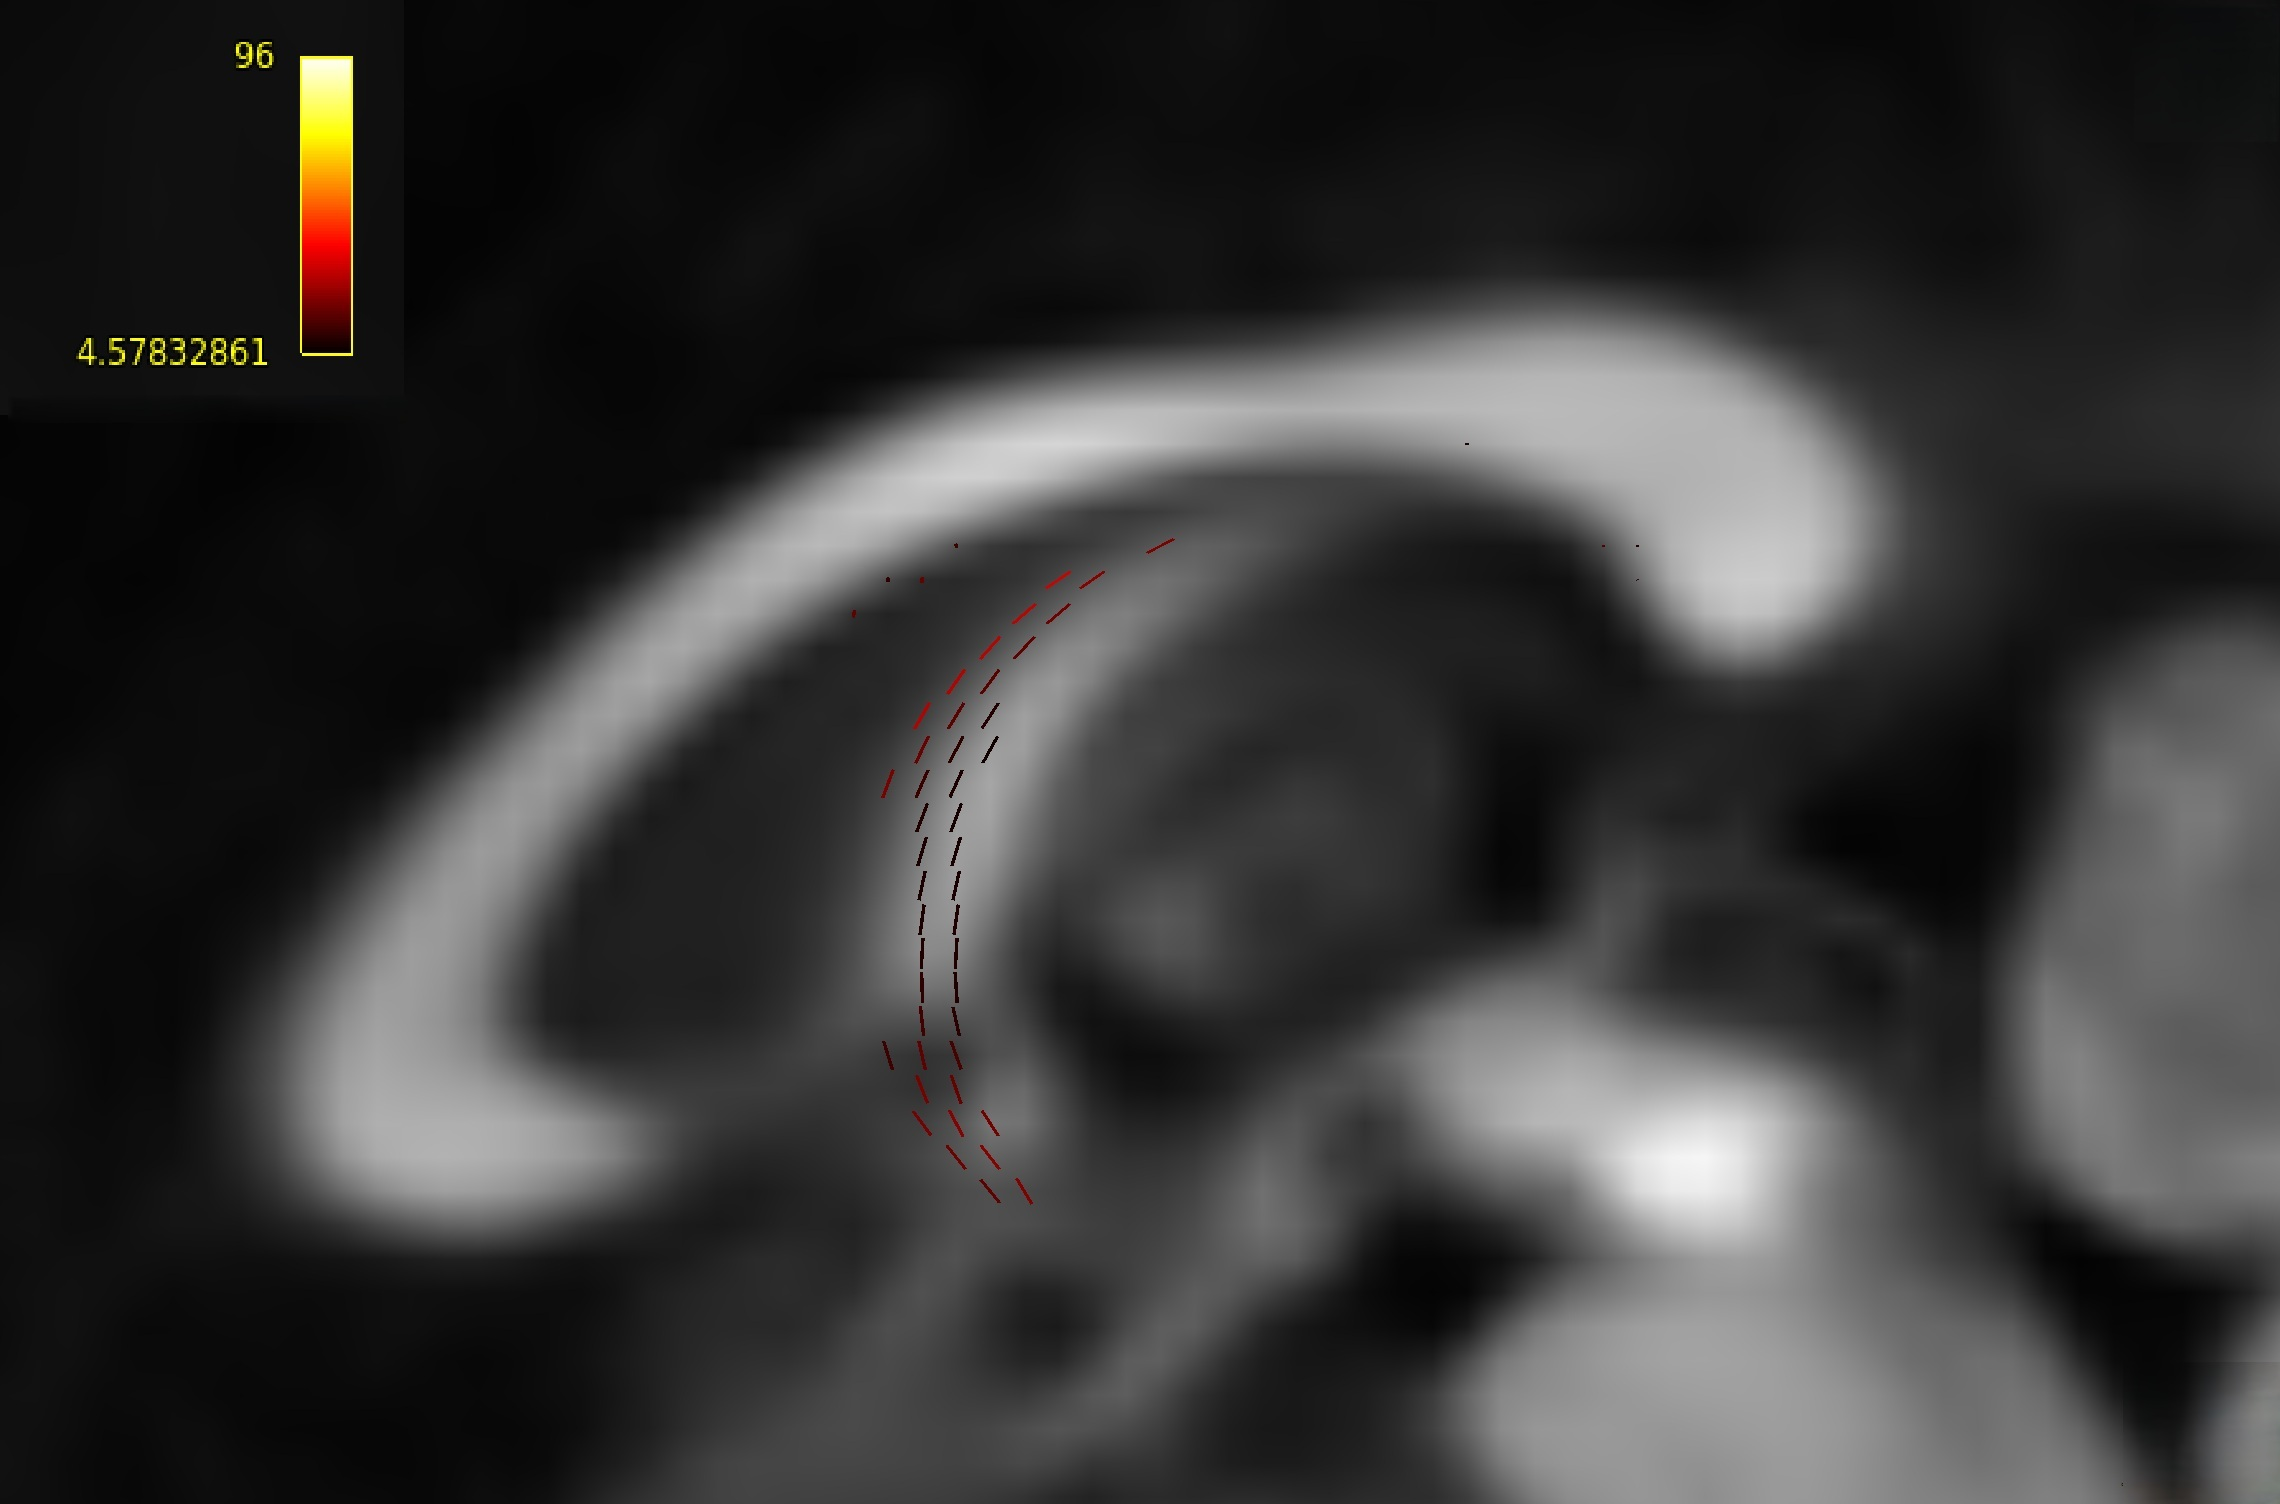
\includegraphics[width=0.8\textwidth]{Images/fornix2.jpg} % or use height= for vertical sizing
  \caption{Fixels derived with MT-CSD. Significant fixels found when testing for higher AFD in the CP group compared to HC. The image shows a zoomed-in view of the fornix, with significant fixels colored by the percentage increase in AFD relative to the average value in the HC group. Since AFD is a relative measure with arbitrary units, the absolute effect size (the difference in mean AFD between groups) is converted to percentage of the HC mean. The increase in the fornix remains small.}
  \label{fig:fornix2}
\end{figure}


\begin{figure}[H]
  \centering
  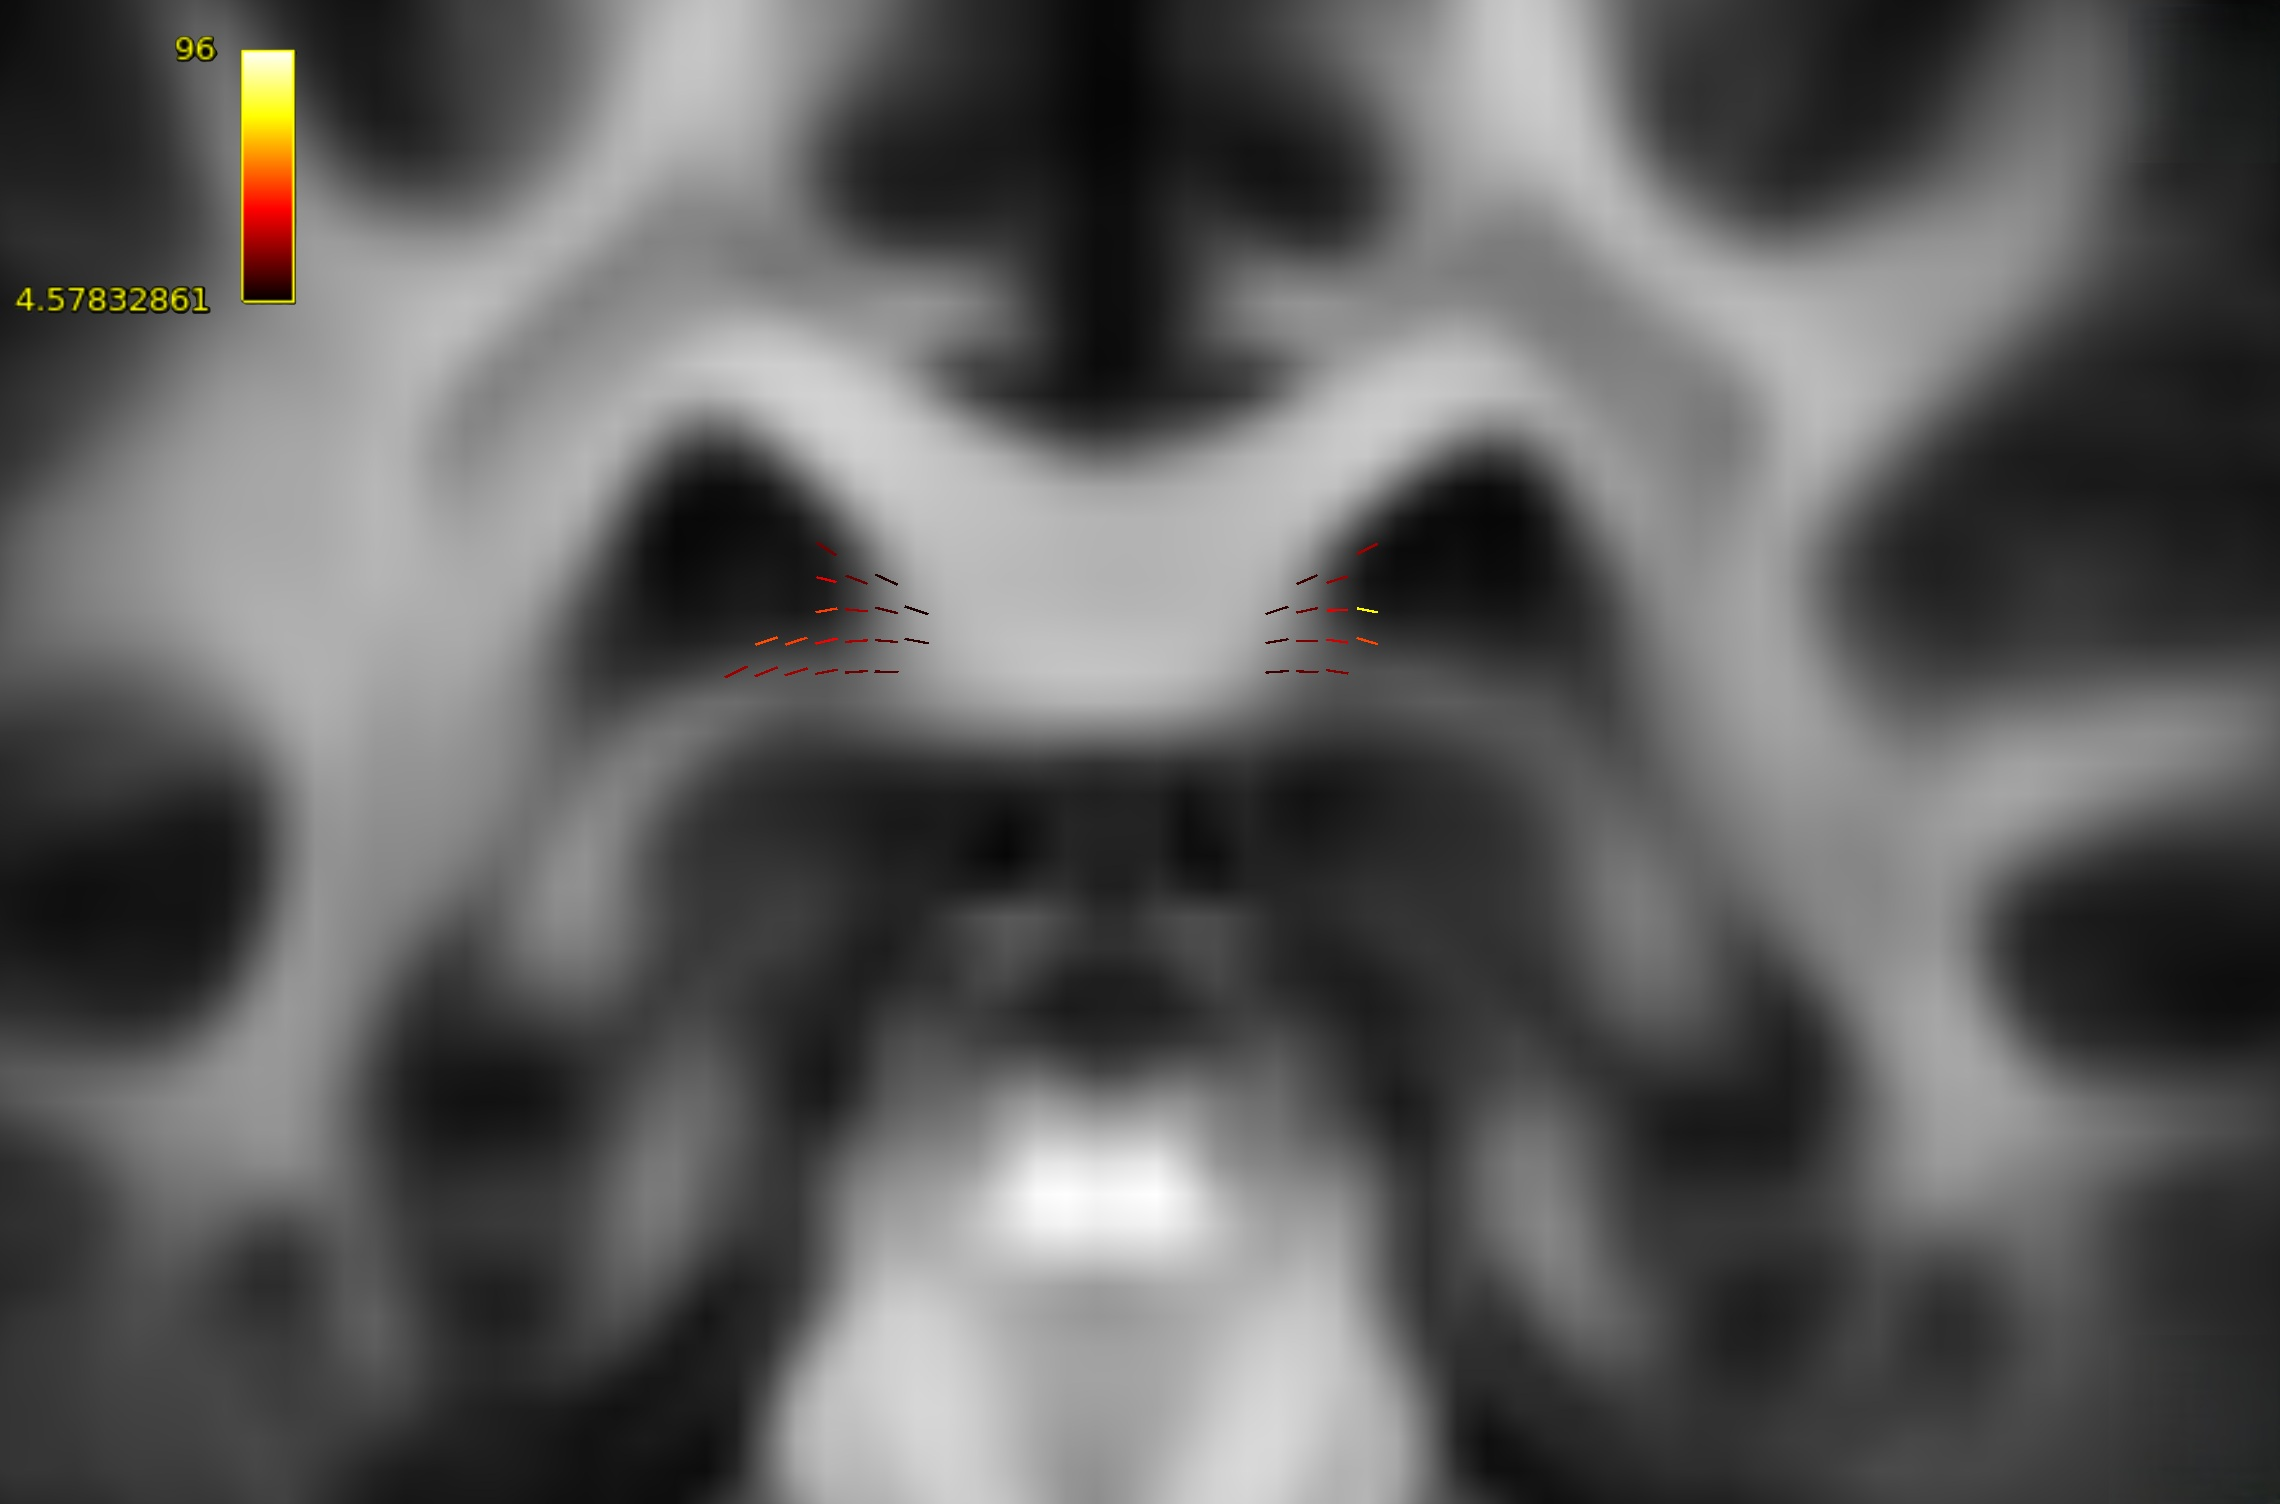
\includegraphics[width=0.8\textwidth]{Images/inter.jpg} % or use height= for vertical sizing
  \caption{Fixels derived with MT-CSD. Significant fixels found when testing for higher AFD in the CP group compared to HC. Detail showing significant fixels at the interface between the corpus callosum and the ventricles, colored by percentage increase in AFD relative to the HC mean. The effect size is larger in regions closer to the ventricles.}
  \label{fig:inter}
\end{figure}

\begin{figure}[H]
    \centering
    \subfloat[Fixels derived with MT-CSD. Results of testing for higher AFD in the CP group compared to HC.]{
        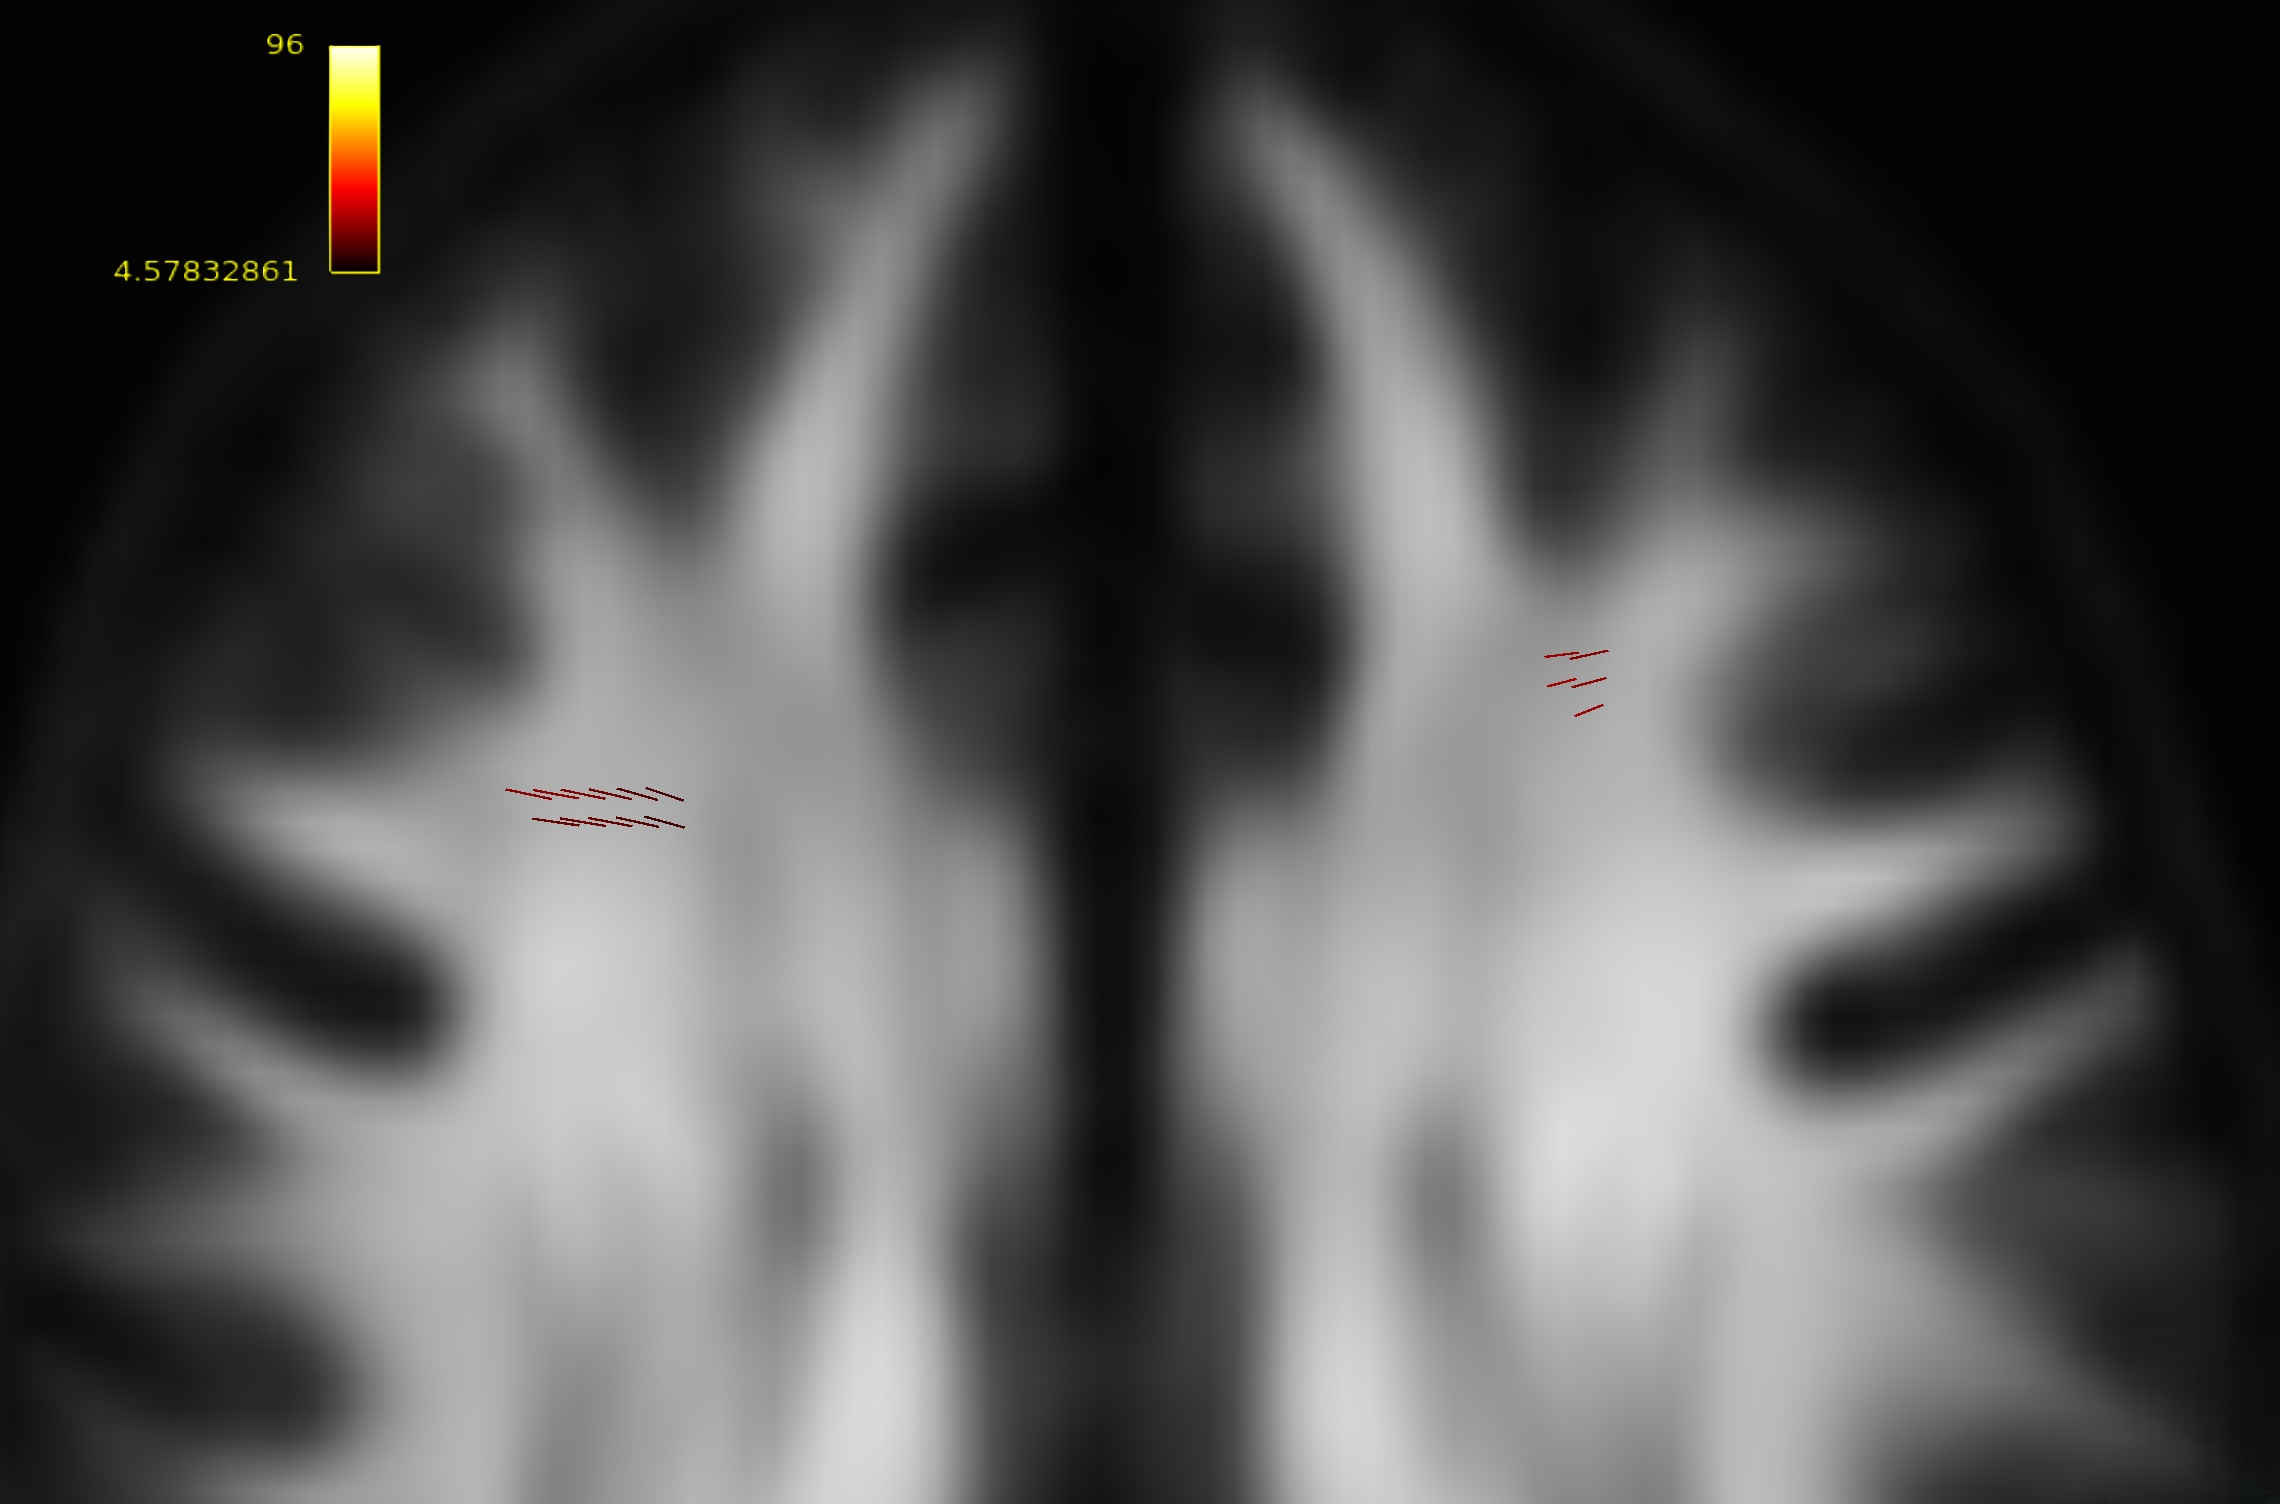
\includegraphics[width=0.45\linewidth]{Images/cross1.jpg}
    \label{fig:subfig-cross1}}
    \hfill
    \subfloat[All fixels included in the fixel mask for the MT-CSD template. Red circles show regions of interest.]{
        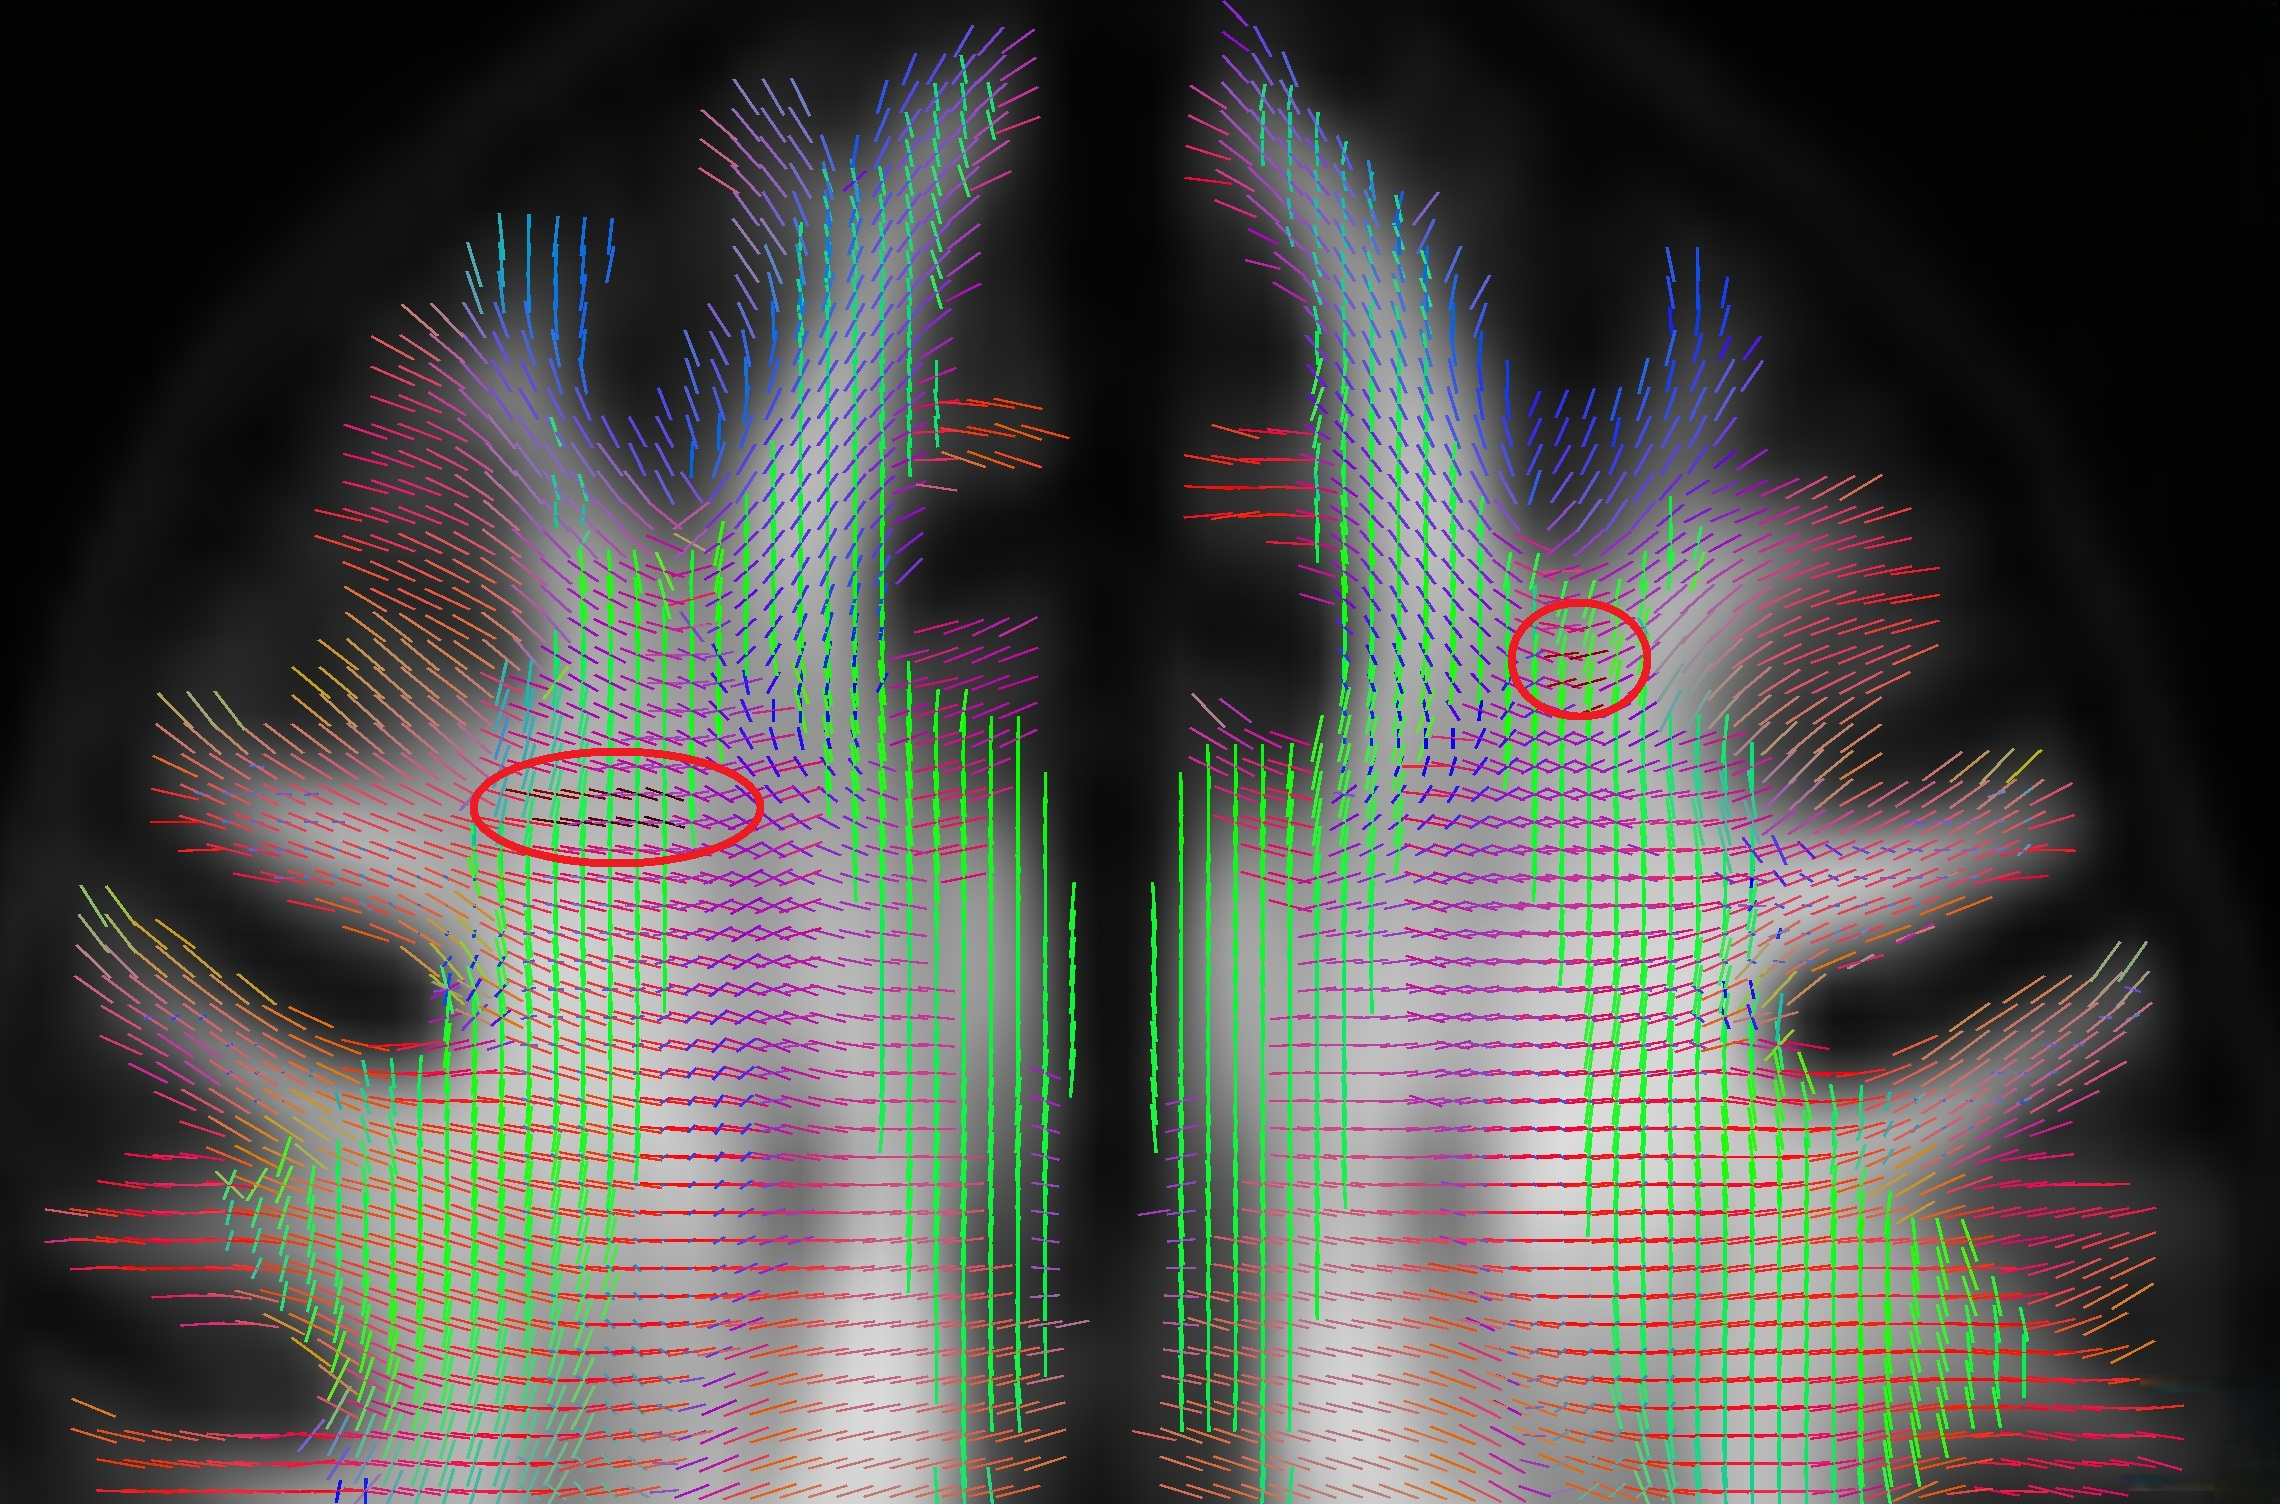
\includegraphics[width=0.45\linewidth]{Images/cross2.jpg}
    \label{fig:subfig-cross2}}
    \caption{(a) significant fixels in crossing regions, colored by percentage increase relative to HC. (b) all fixels in the mask, colored by directionality. Red circles indicate the crossing fibre regions where significant fixels were found.}
    \label{fig:cross}
\end{figure}


\subsection{LoRE-SD}
Different scaling contrasts applied to the ODFs produced varying outcomes of the statistical analysis.
When using the intra-axonal contrast for scaling, significant fixels were observed only for the AFD metric, and exclusively when testing for an increase in CP compared to HC. A total of 16 significant fixels were identified. No significant fixels were found for the other two metrics. The significant fixels and a comparison with the results when using MT-CSD in the same region  are shown in Figure~\ref{fig:Lore_comp}. 


\begin{figure}[h]
    \centering
    \subfloat[LoRE-SD with intra-axonal scaling]{
        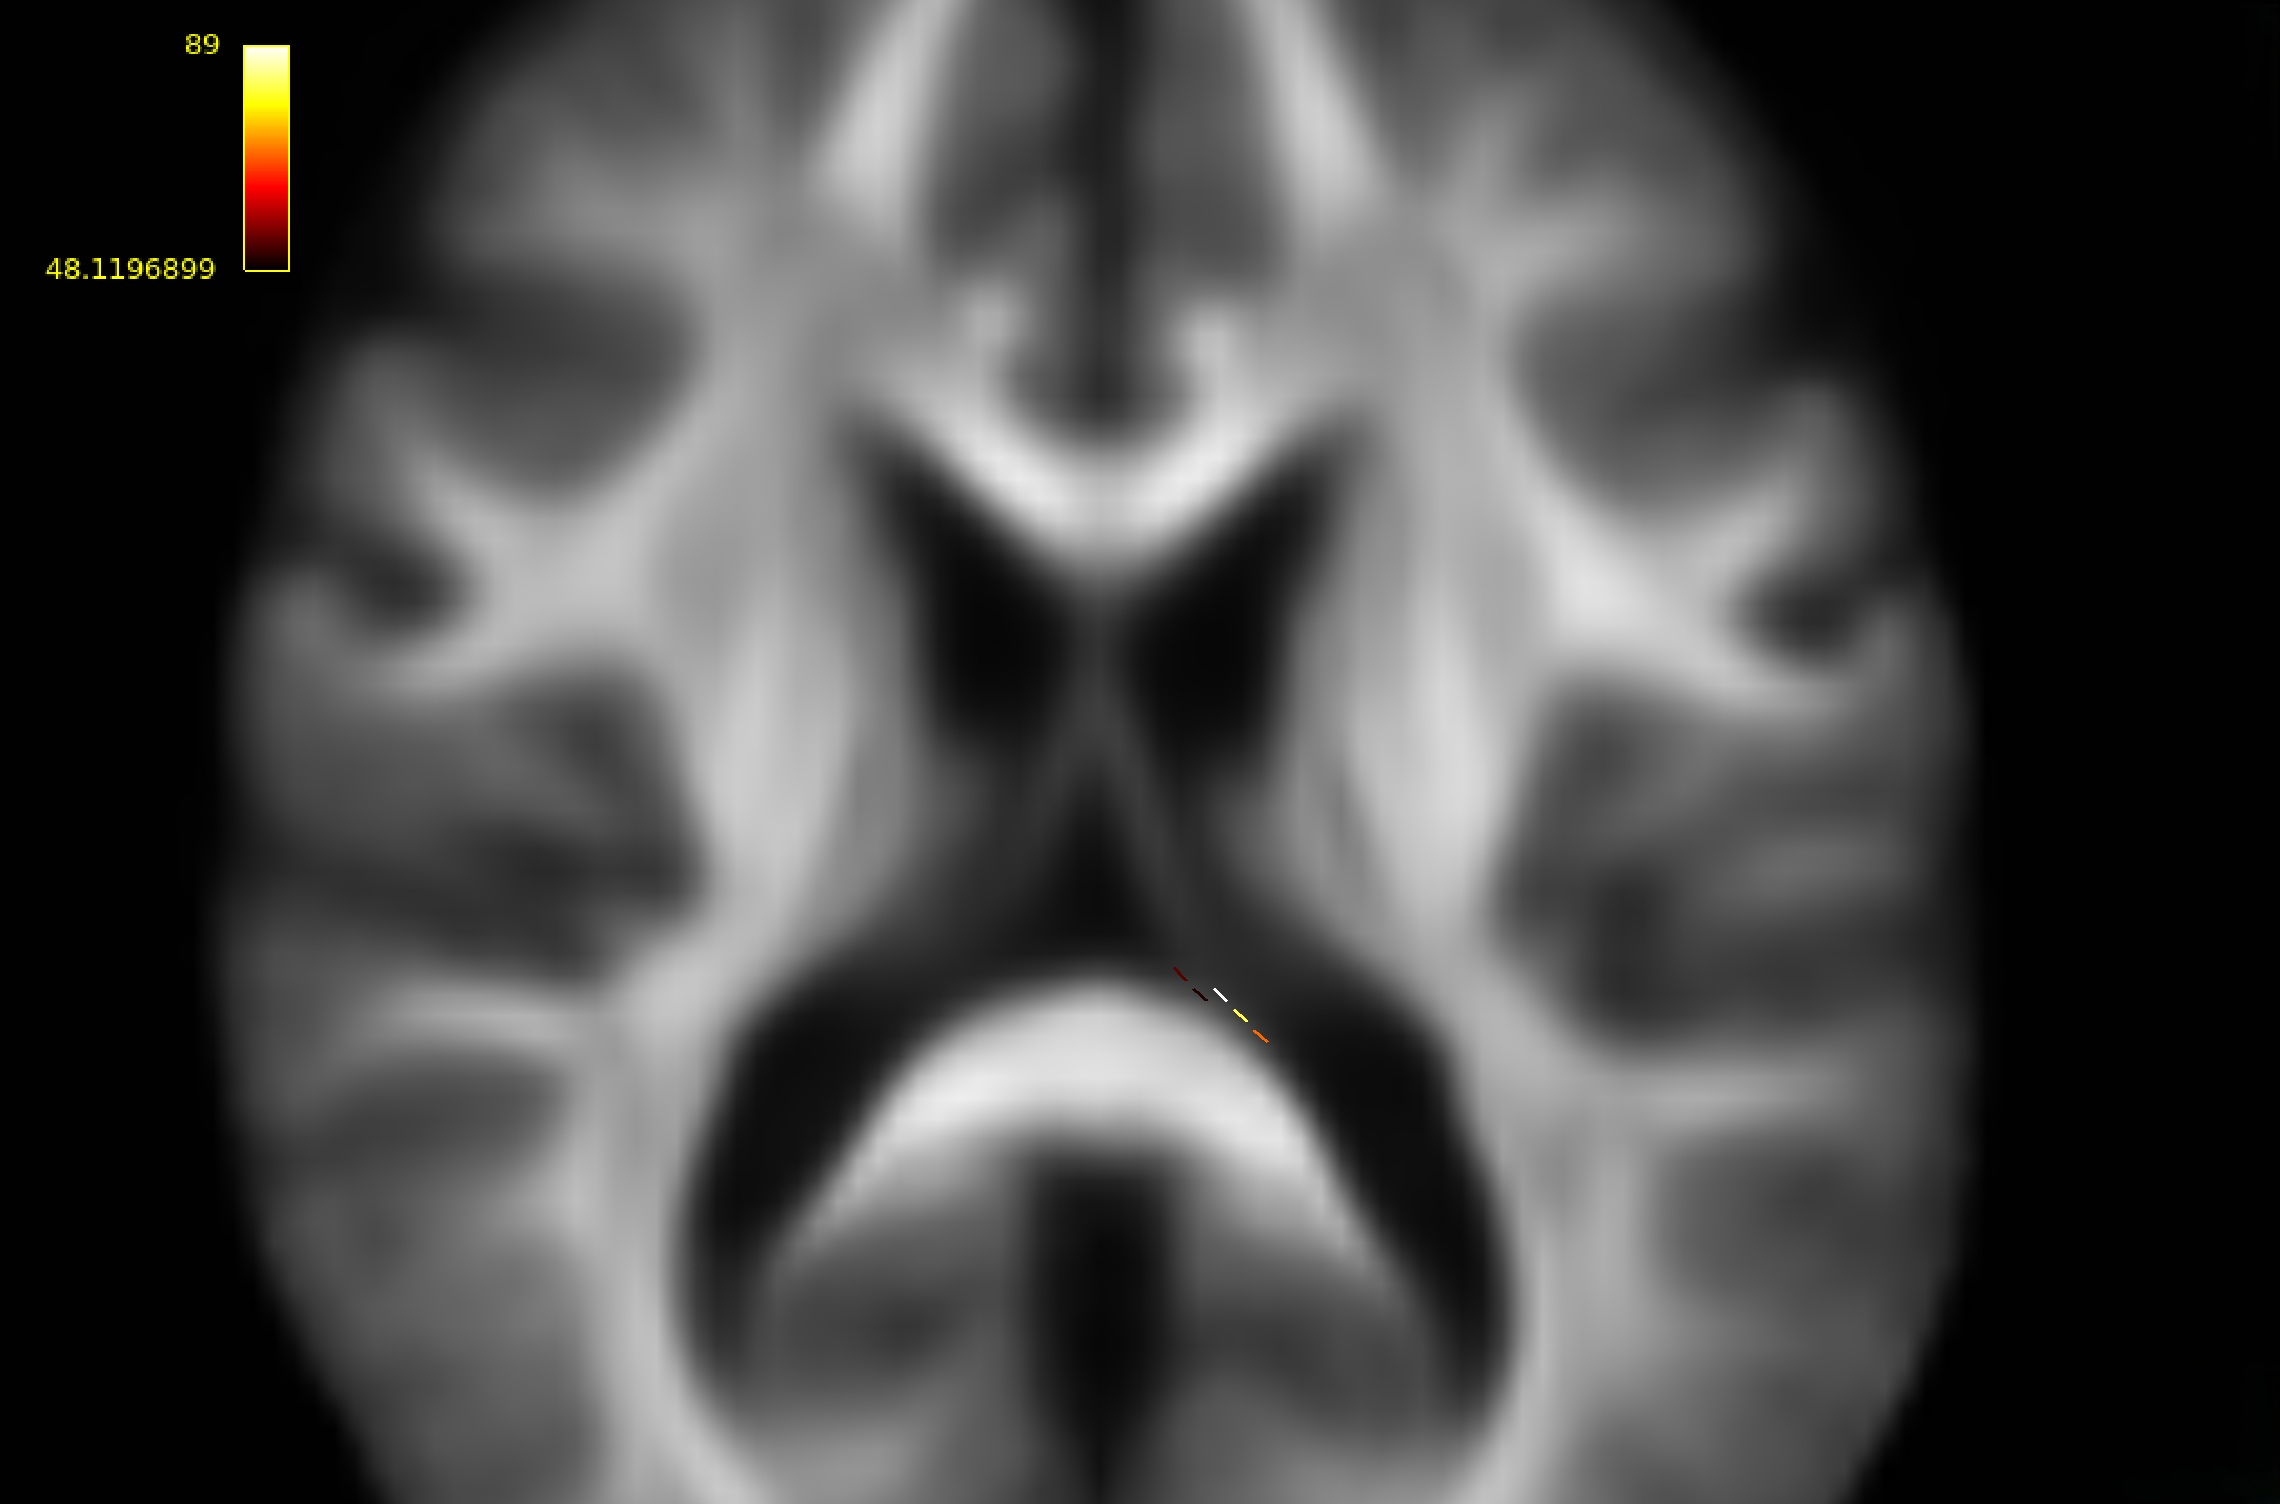
\includegraphics[width=0.45\linewidth]{Images/comp_final_intra.jpg}
        \label{fig:subfig-lore-intra}
    }
    \hfill
    \subfloat[MT-CSD]{
        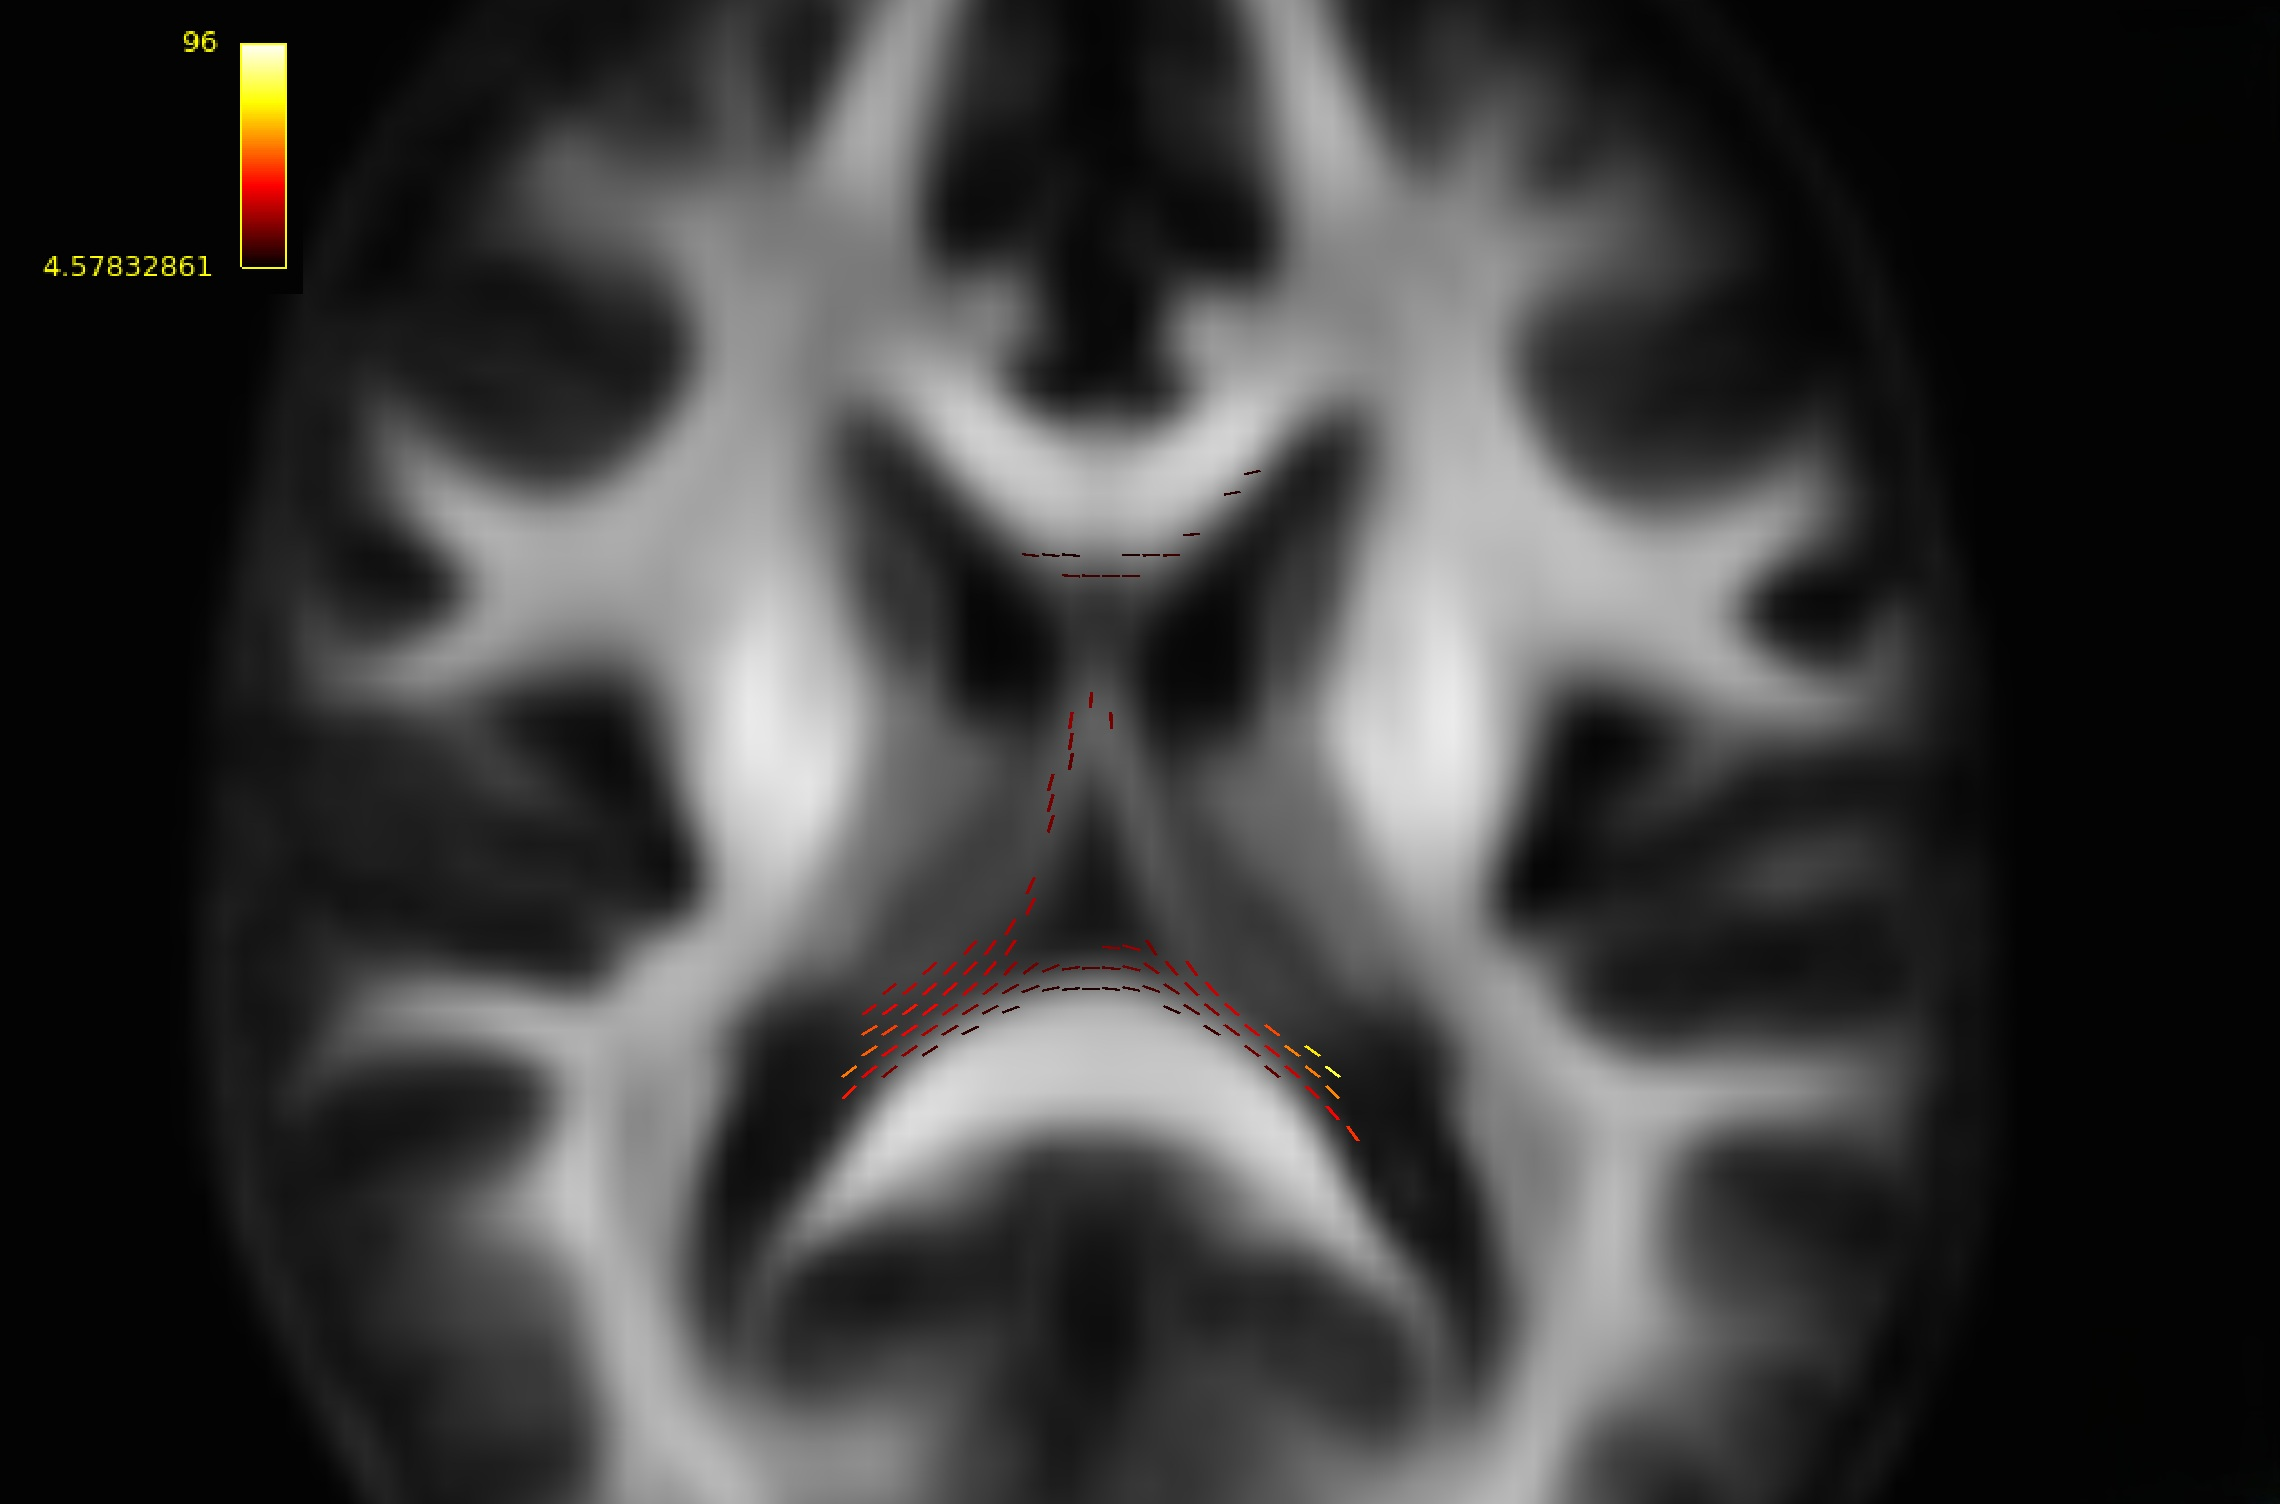
\includegraphics[width=0.45\linewidth]{Images/comp_final_MT.jpg}
        \label{fig:subfig-mtcsd}
    }
    \caption{Left: LoRE-SD scaled with the intra-axonal contrast, testing for higher AFD in CP compared to HC. The fixels highlight a region at the interface with the ventricles. Right: significant fixels in the same area for MT-CSD for the same test, including fixels in the fornix and CC.}
    \label{fig:Lore_comp}
\end{figure}


With the FA and the anisotropic-intra-axonal contrast no significant results were found. Finally for the WM contrast we found a significant increase of AFD in CP compared to HC. Only 78 fixels were found to be significant. Similarly to MT-CSD, the fixels were part of the fornix and at the tissue interface with the ventricles, but no significance was found in the crossing fibre regions. Significant results are in Figure~\ref{fig:fornix4} and ~\ref{fig:wm_result}. No differences where found for the other group comparisons or for the other two metrics.


\begin{figure}[H]
    \centering
    \subfloat[Sagittal view.]{
        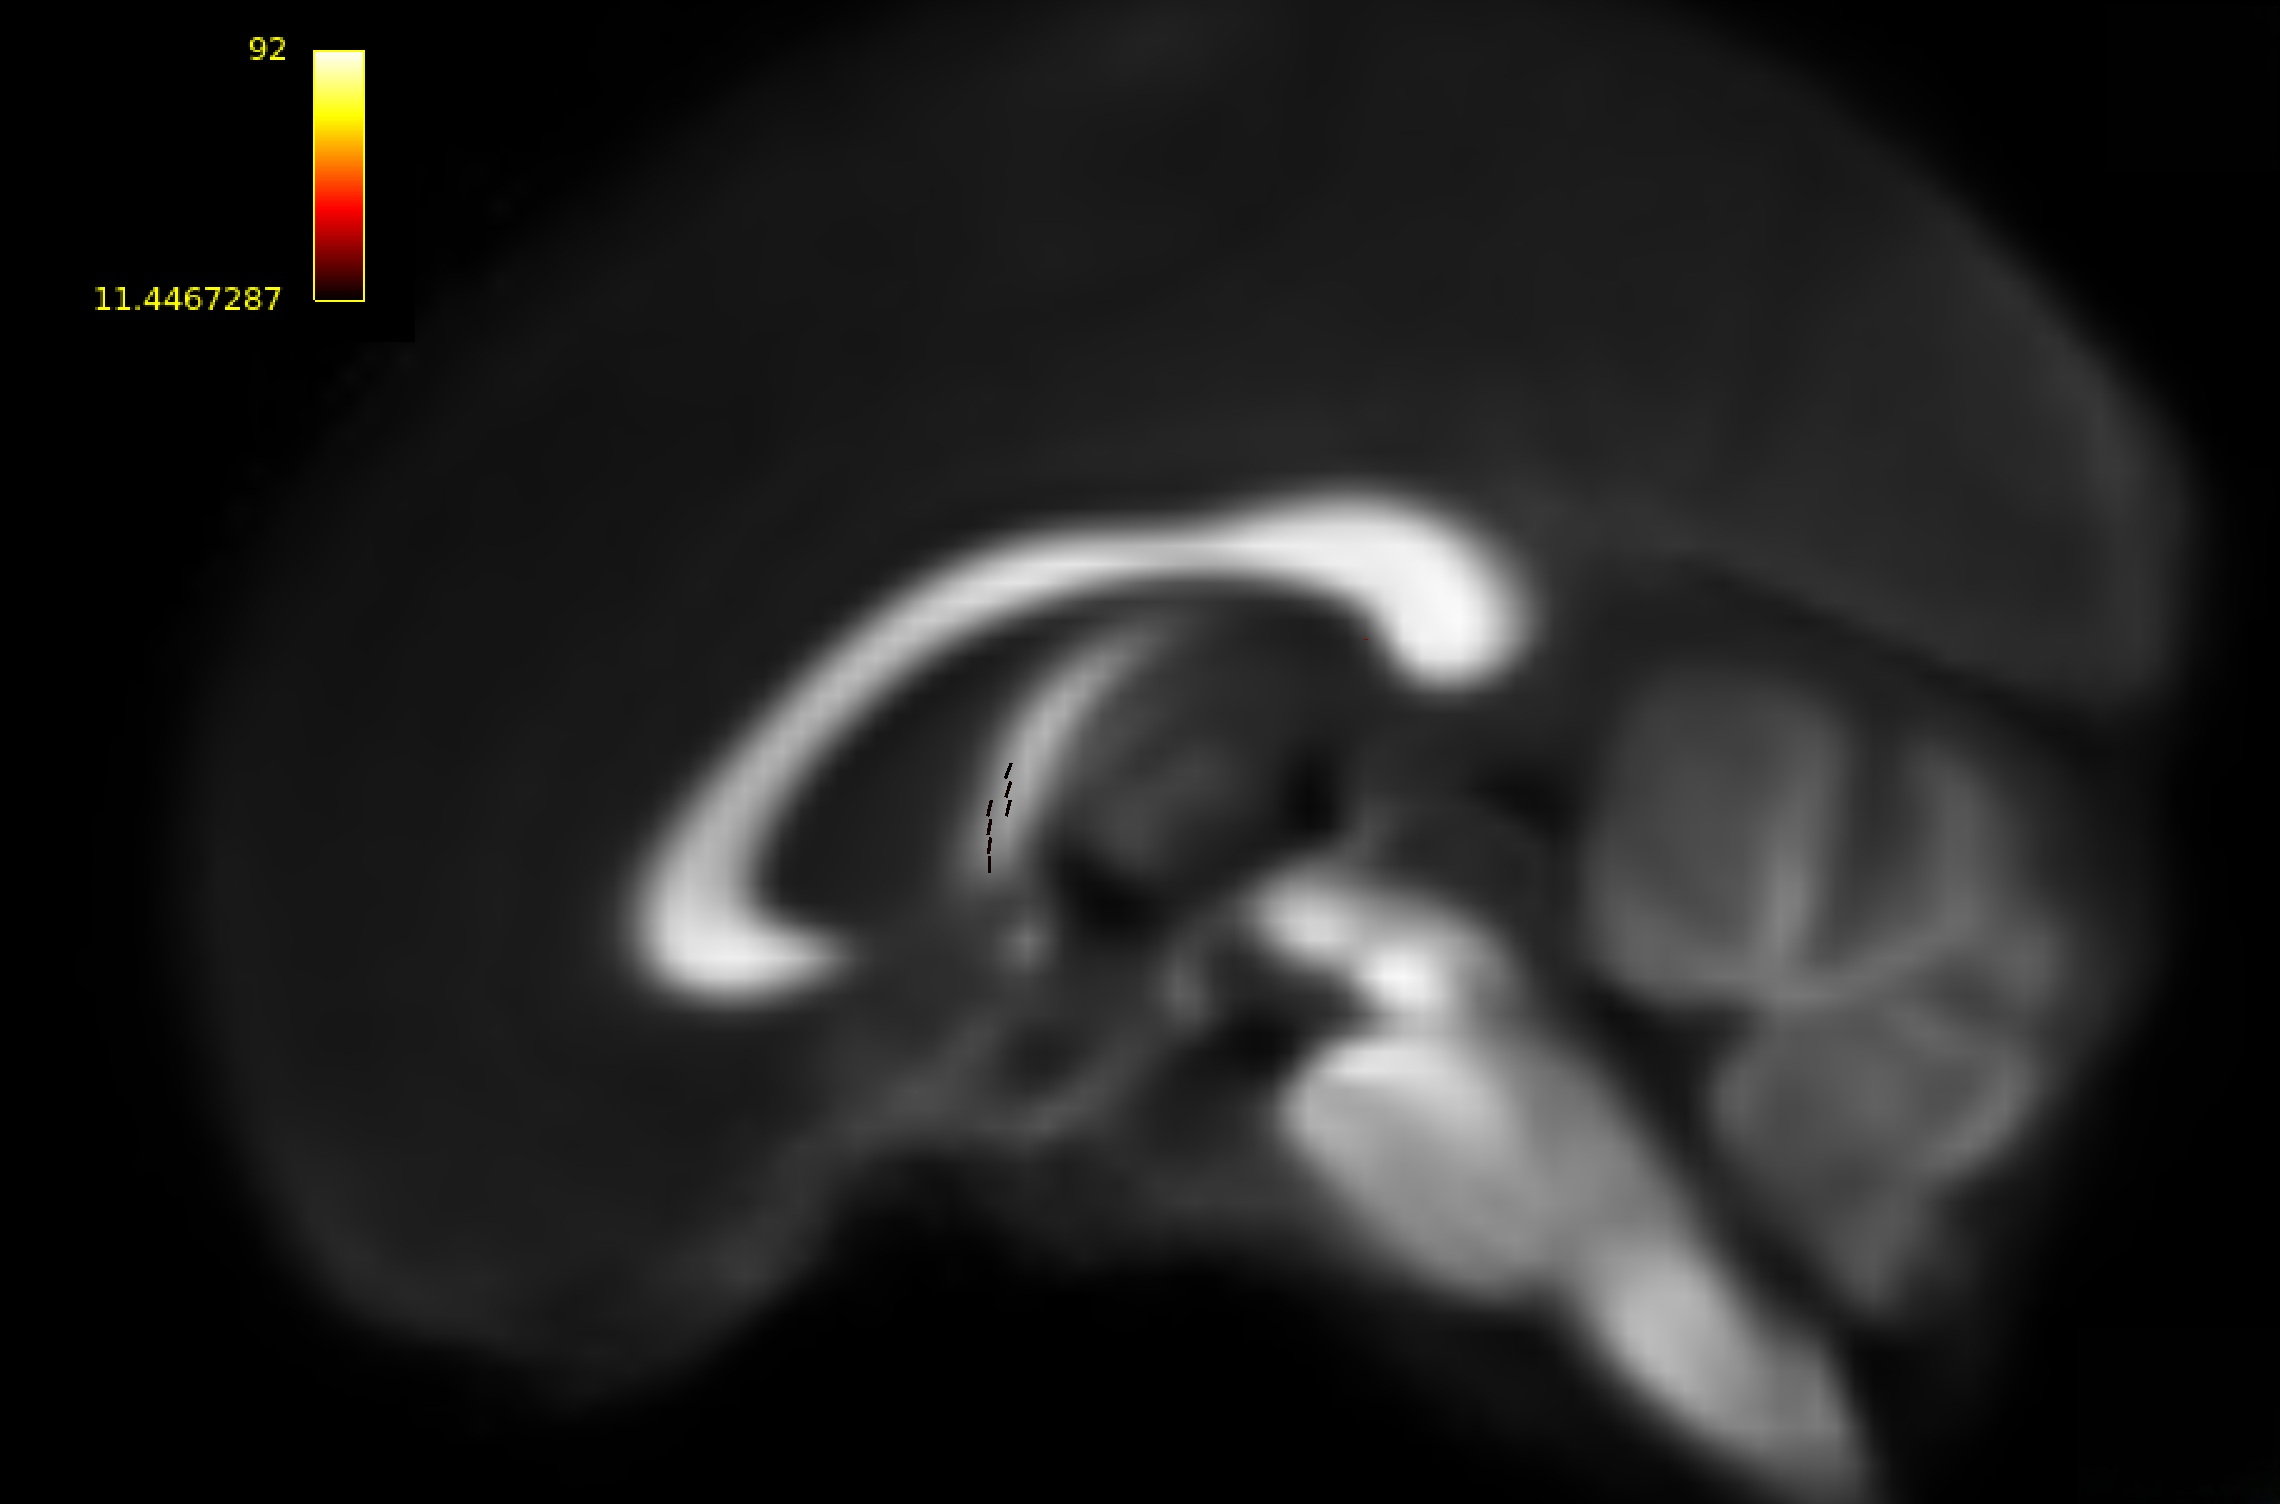
\includegraphics[width=0.45\linewidth]{Images/new_wm0000.jpg}
        \label{fig:subfig-sagittal}
    }
    \hfill
    \subfloat[Coronal view.]{
        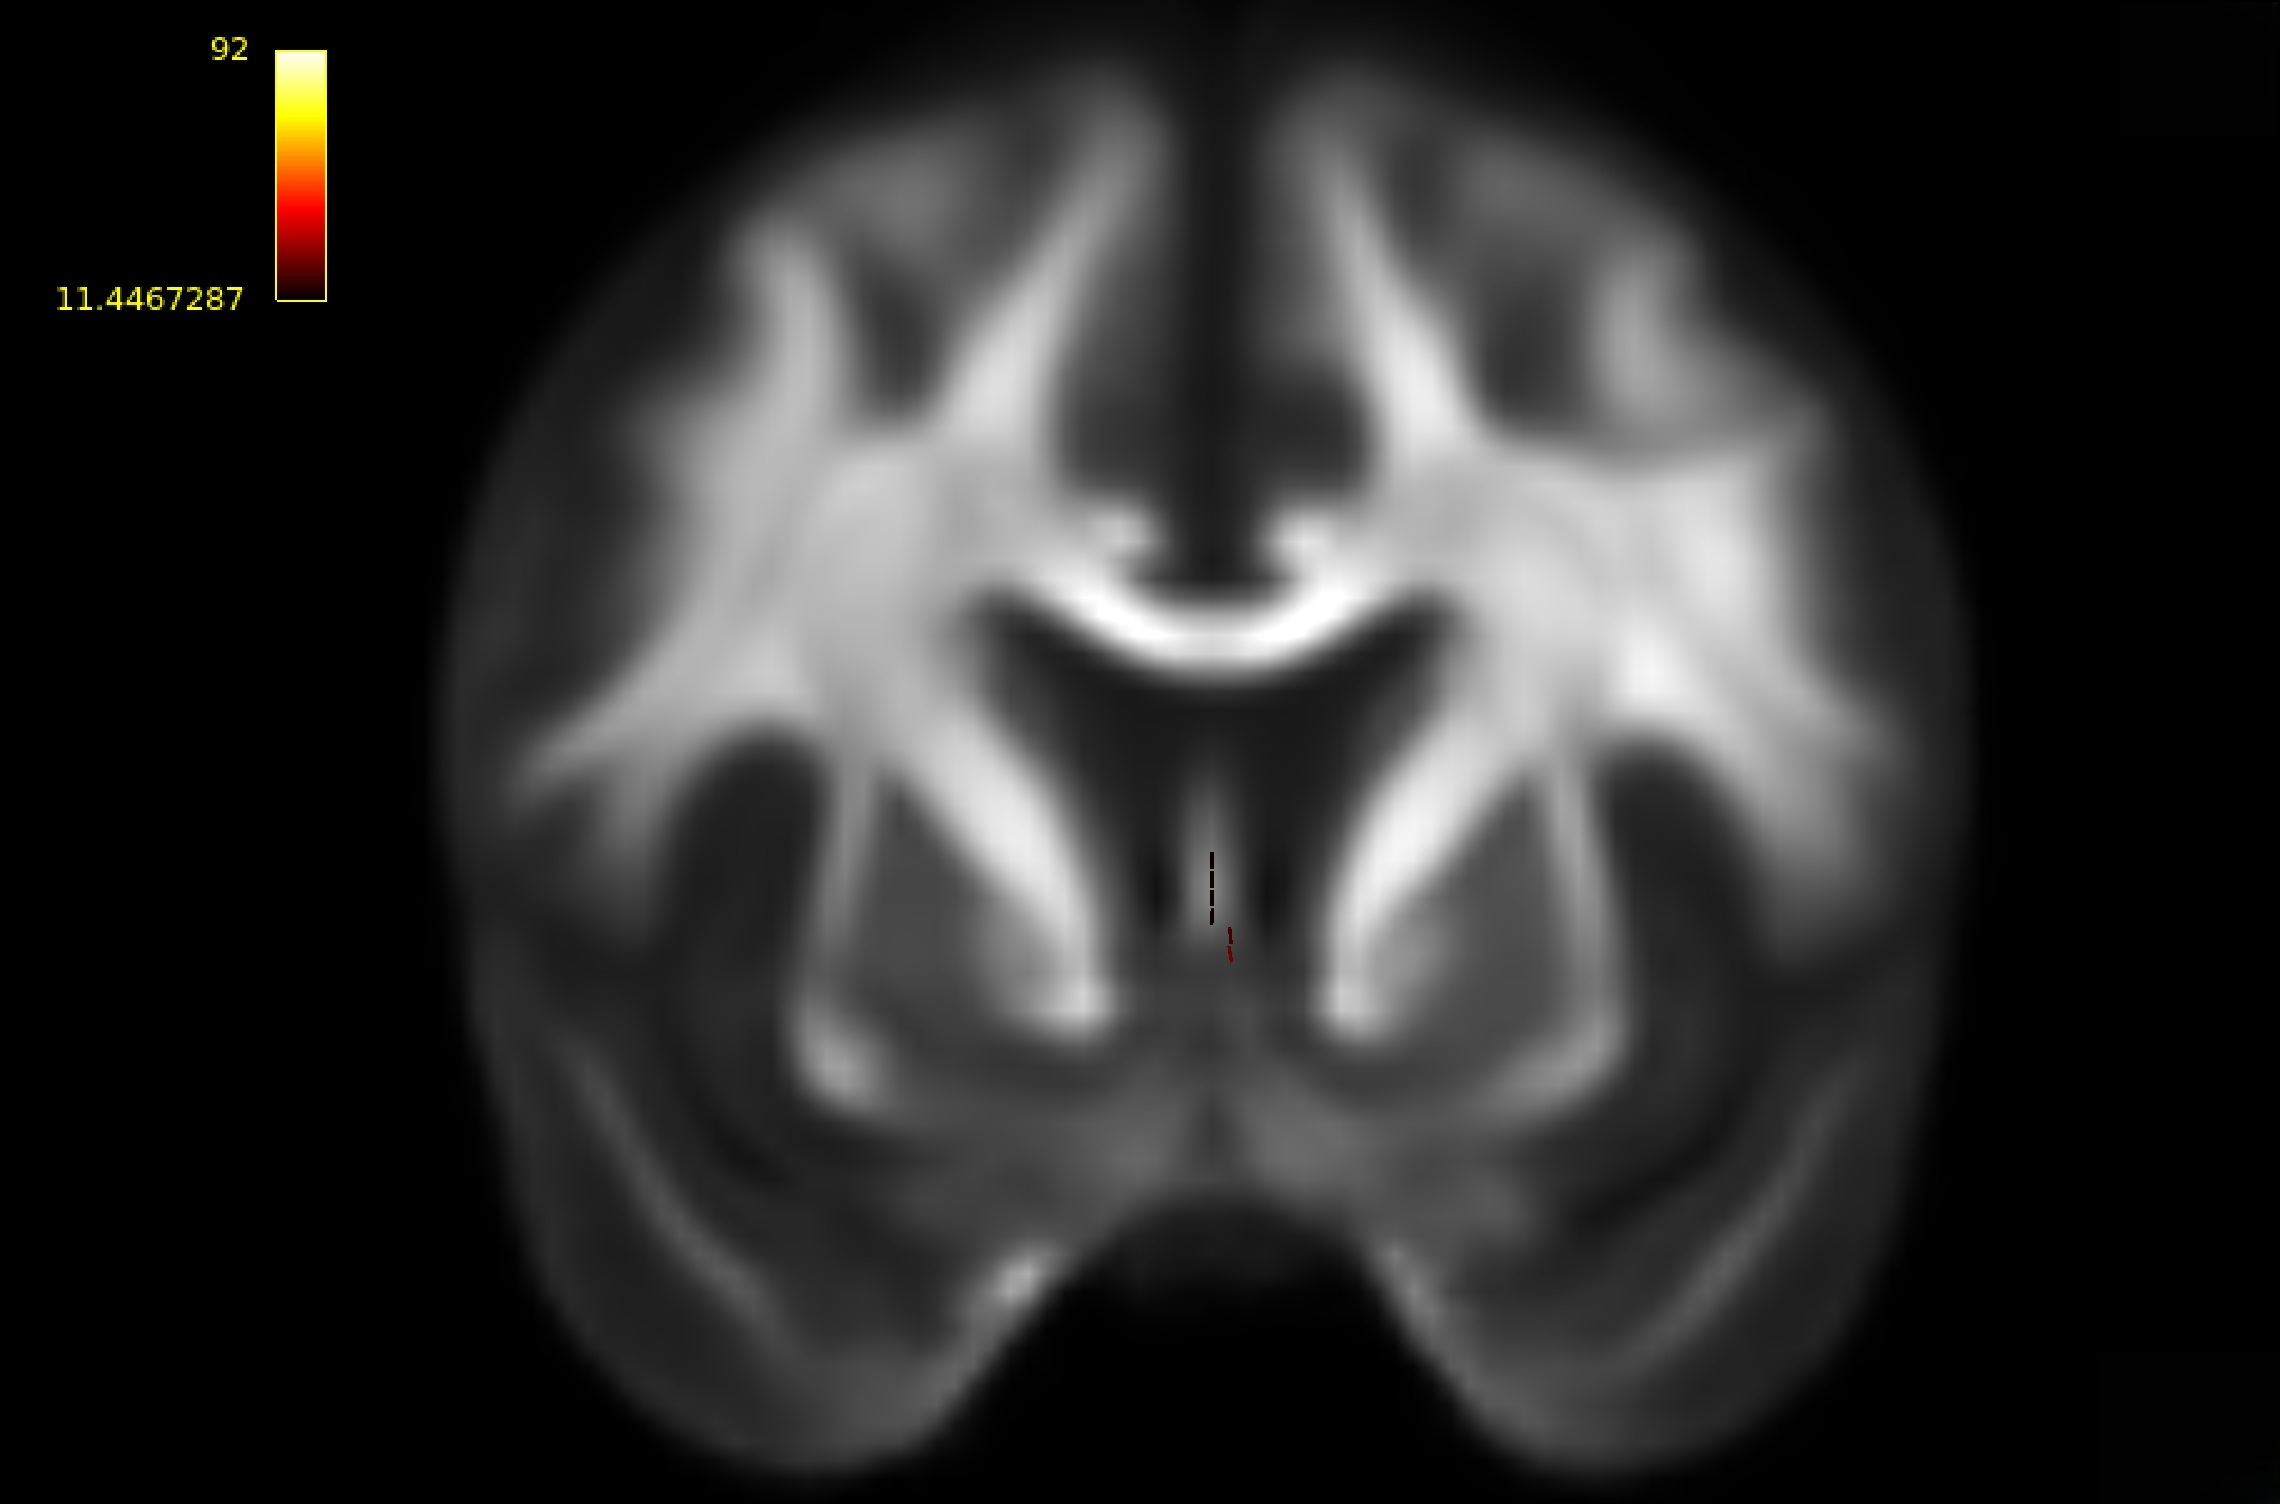
\includegraphics[width=0.45\linewidth]{Images/new_wm0001.jpg}
        \label{fig:subfig-coronal}
    }
    \caption{Fixels extracted from LoRE-SD scaled with the WM contrast, testing for higher AFD in CP compared to HC. The background image is the average WM contrast across all subjects in template space. Only significant fixels are shown, with color indicating the percentage increase relative to HC. Fixels belong to the fornix.}
    \label{fig:fornix4}
\end{figure}



\begin{figure}[h]
  \centering
  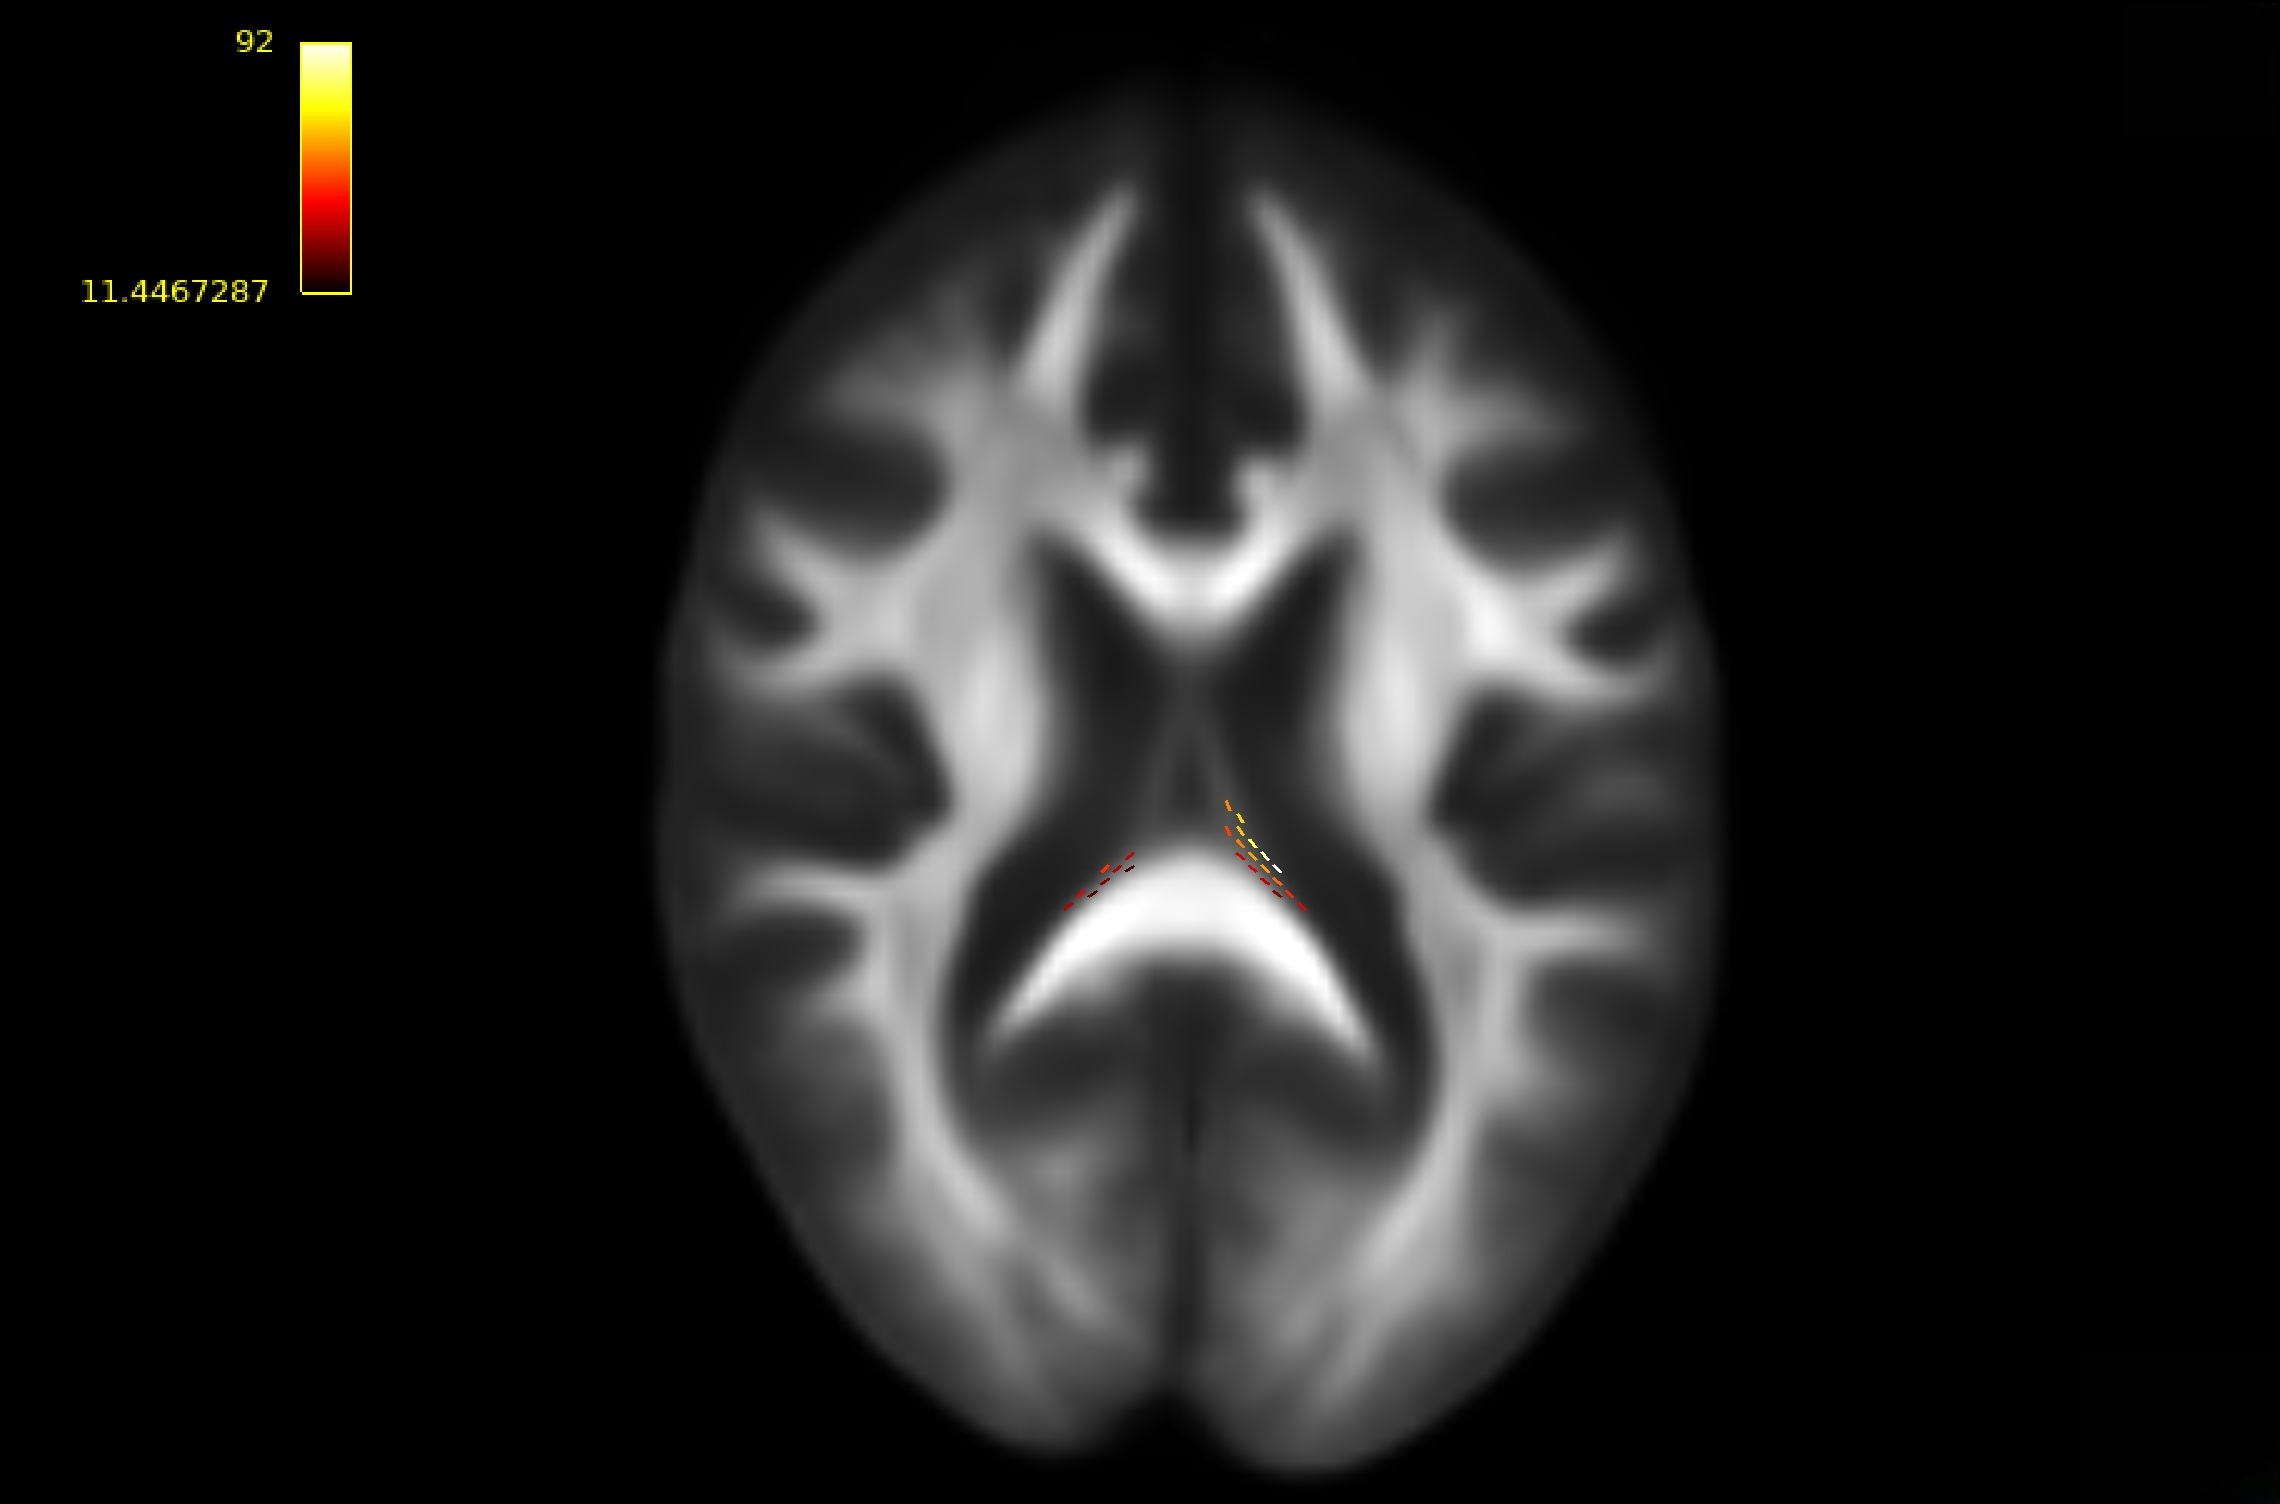
\includegraphics[width=0.9\textwidth]{Images/new_wm0002.jpg} % or use height= for vertical sizing
  \caption{LoRE-SD scaled with the WM contrast, testing for higher AFD in CP compared to HC. Only significant fixels are shown and the color represents the percentage increase relative to HC. The image in the background is the average WM contrast across all subjects in template space. Fixels are part of the fornix, corpus callosum and interface with the ventricles.}
  \label{fig:wm_result}
\end{figure}

\subsection{Results with reduced fixel mask}
To reduce the number of fixels and increase statistical power, a threshold was applied to include only fixels with a sufficient number of streamlines passing through them, before repeating the analysis. For MT-CSD ODFs, a threshold of 250 streamlines was used. This reduced the total number of fixels in the analysis mask from 287,483 (after excluding the cerebellum and brainstem) to 157,821, while preserving overall WM connectivity, as no major fibre bundles were excluded. Figure~\ref{fig:reduced} illustrates the fixels excluded by this thresholding process, which were predominantly located in regions of complex fibre crossings and at tissue boundaries.

\begin{figure}[h]
    \centering
    \subfloat[Sagittal view]{
        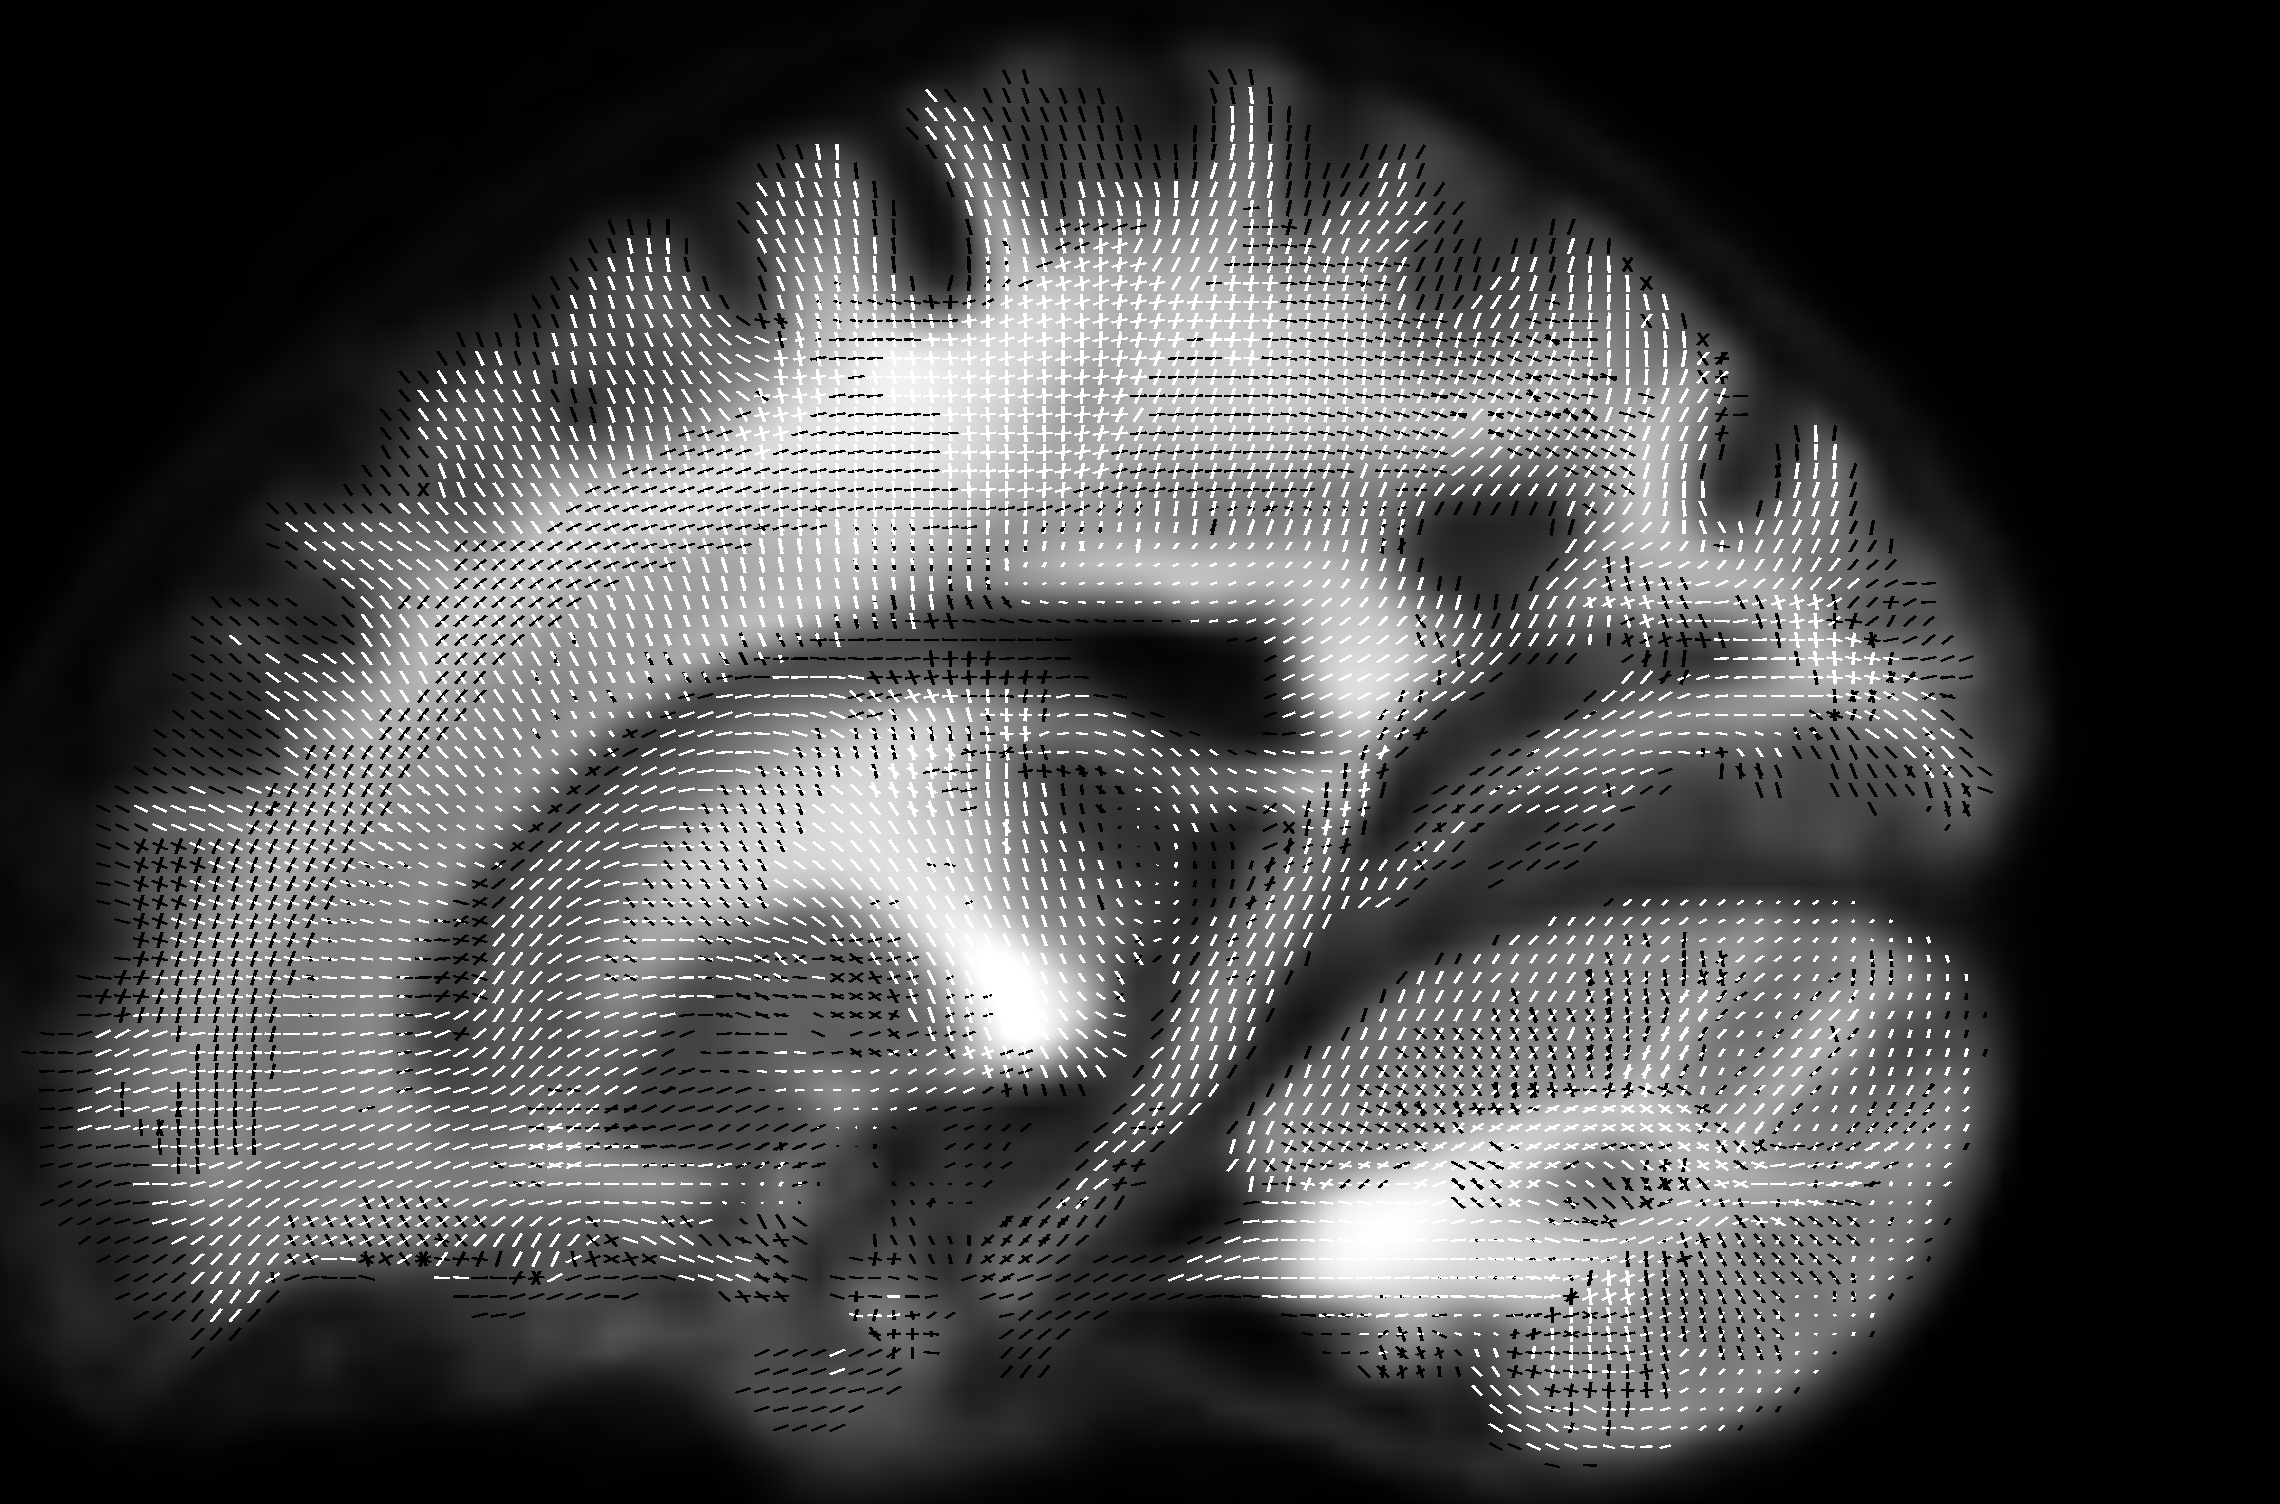
\includegraphics[width=0.5\linewidth]{Images/250_mask_MT0000.jpg}
        \label{fig:subfig-sagittal-mask}
    }
    \hfill
    \subfloat[Coronal view]{
        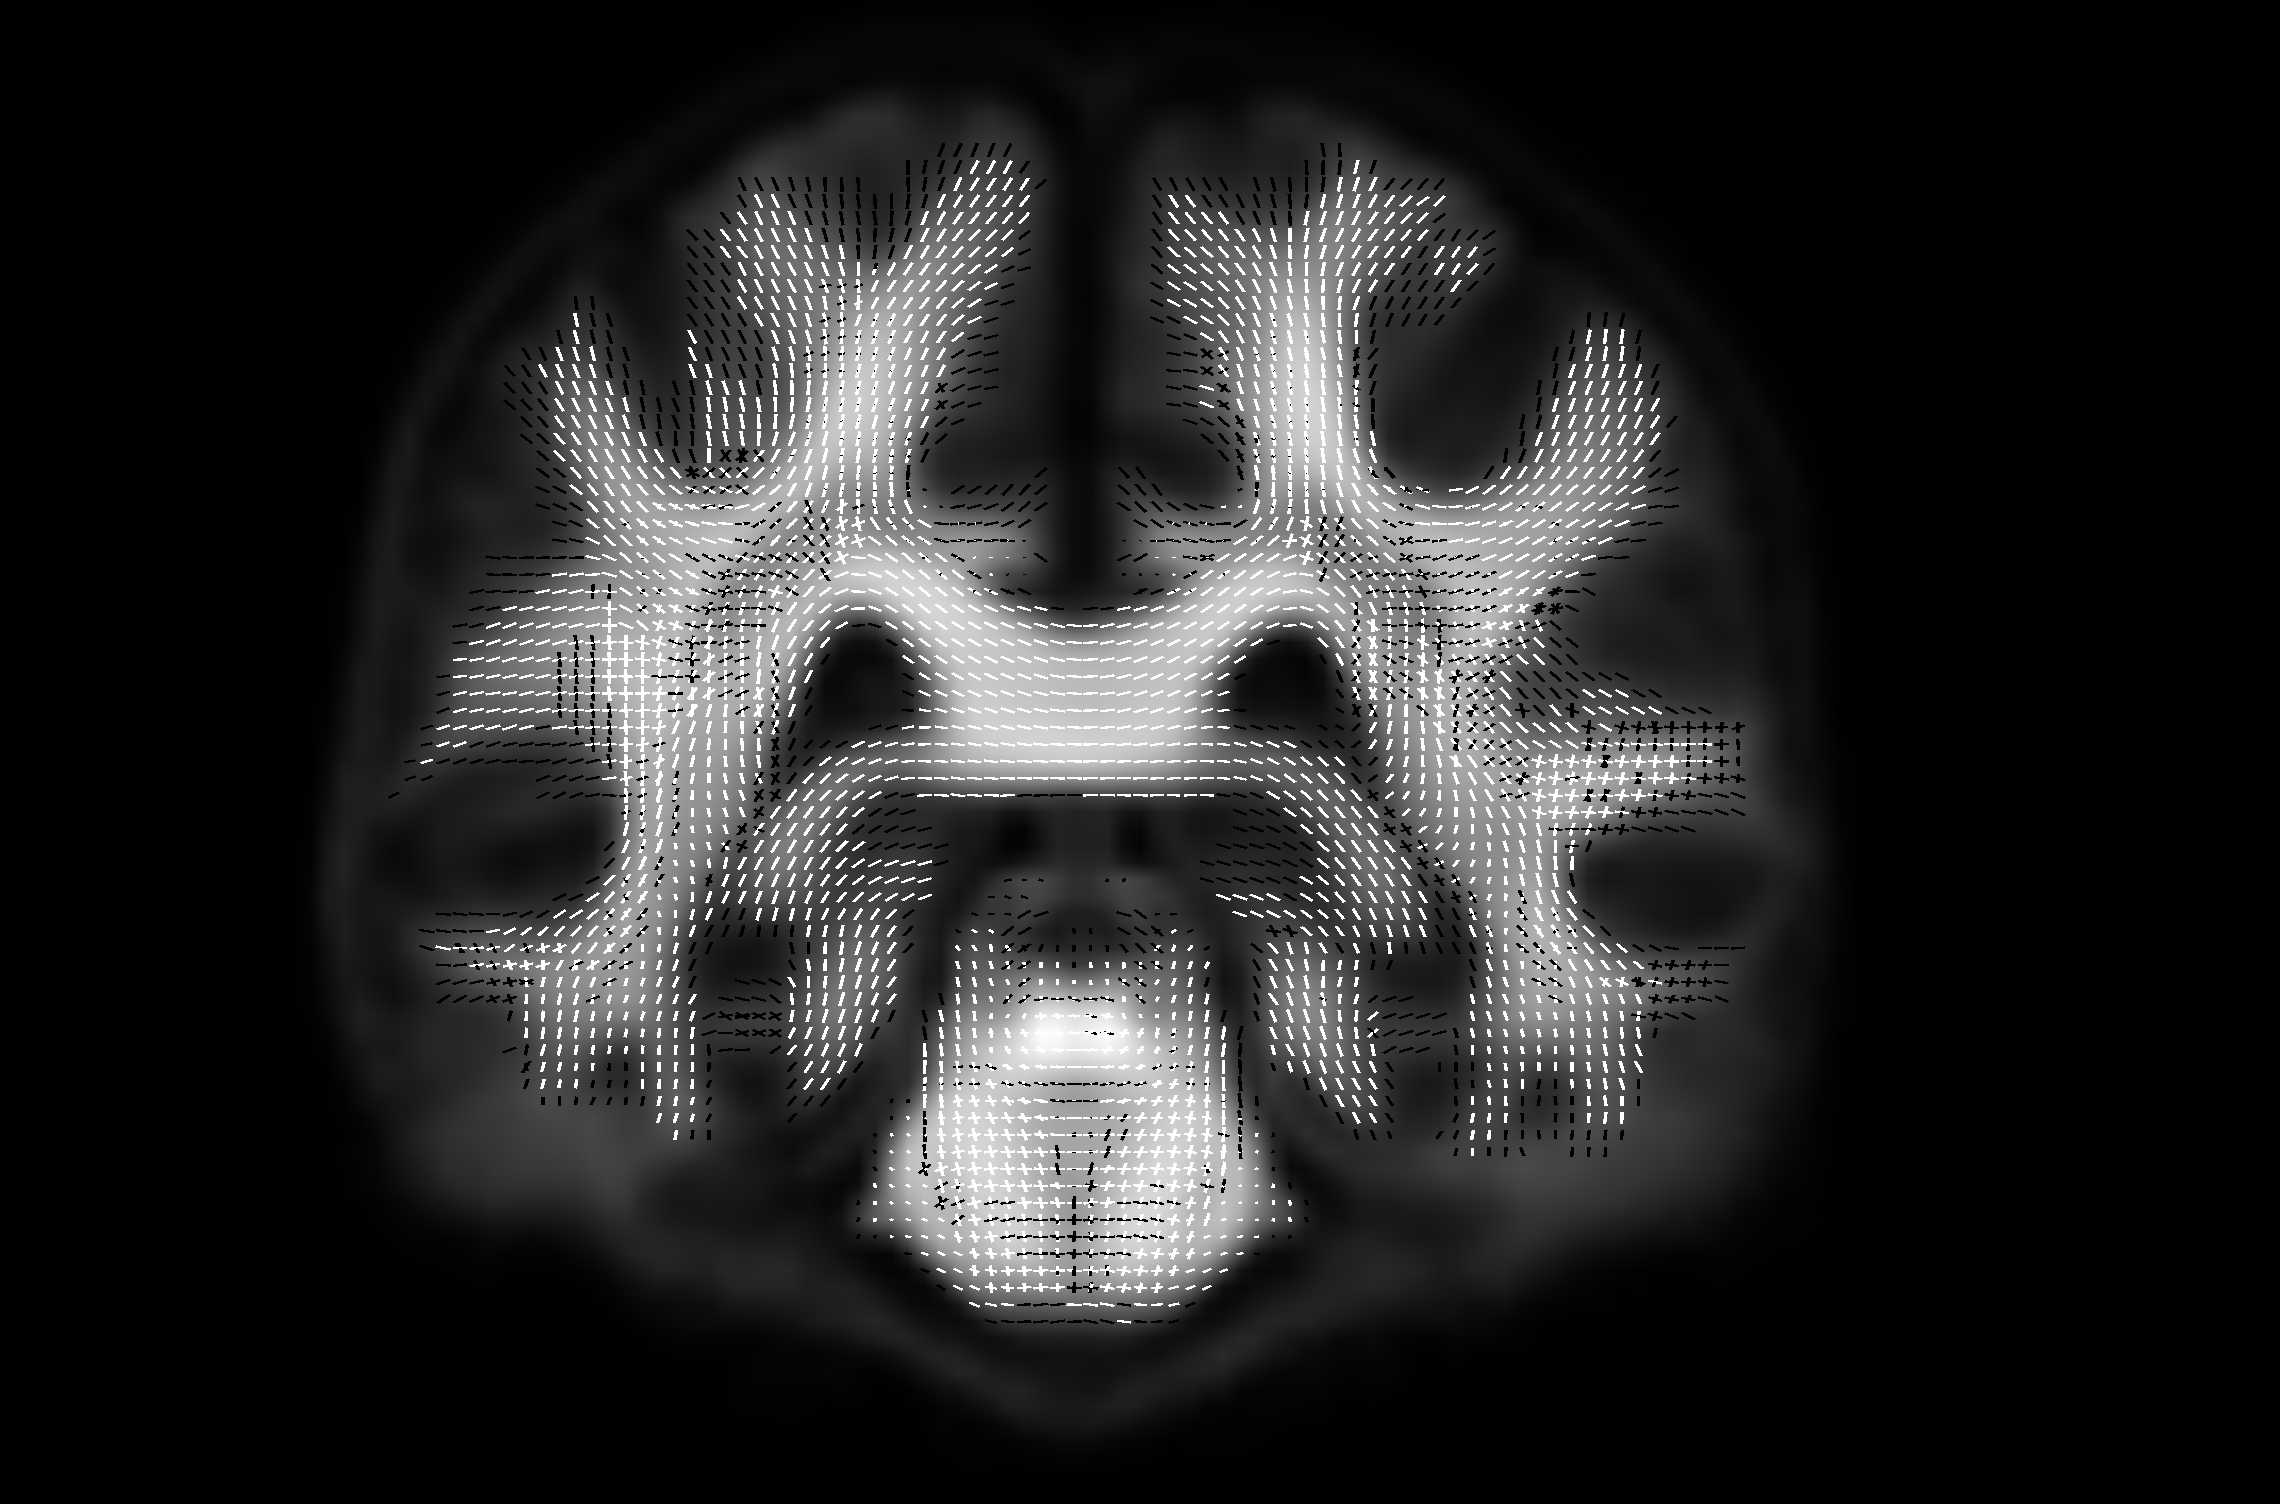
\includegraphics[width=0.5\linewidth]{Images/250_mask_MT0009.jpg}
        \label{fig:subfig-coronal-mask}
    }
    \caption{Reduced fixel mask for the MT-CSD-derived template after applying a threshold on the number of streamlines. Only fixels with more than 250 streamlines passing through them are retained (shown in white); excluded fixels are shown in black.}
    \label{fig:reduced}
\end{figure}


For the AFD metric, after excluding low-density fixels based on streamline count ($\geq$250), we identified 868 fixels showing a significant increase in the CP group compared to HC. No other contrasts gave significant results for AFD. Examples of these findings are presented in Figure~\ref{fig:reduced_MT}. Notably, the maximum effect size decreased with the reduced mask, and fewer significant fixels were detected at tissue interfaces, likely due to the exclusion of possible spurious fibres in these regions. In contrast, there was a relative increase in significant fixels within the CC.

\begin{figure}[H]
    \centering
    \subfloat[Reduced Fixel Mask]{
        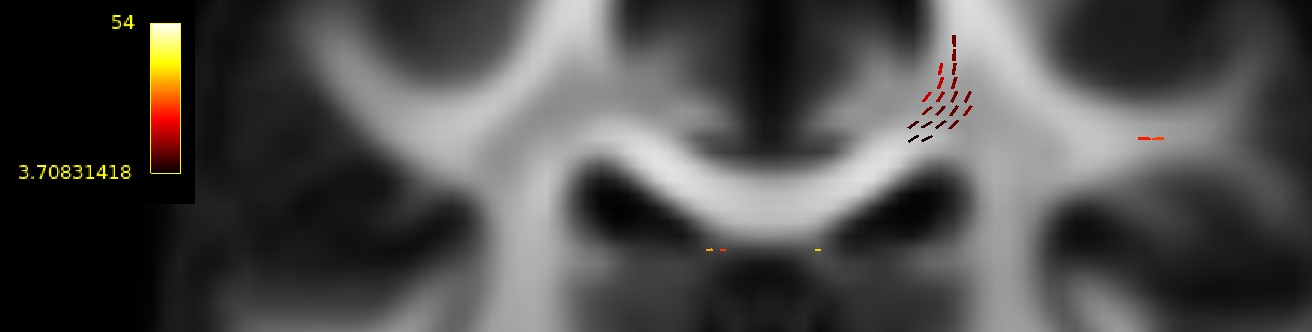
\includegraphics[width=0.8\linewidth]{Images/comp_TDI1.jpg}
        \label{fig:subfig-reduced-fixel}
    } \\[1em] % line break + vertical space
    \subfloat[Full Mask]{
        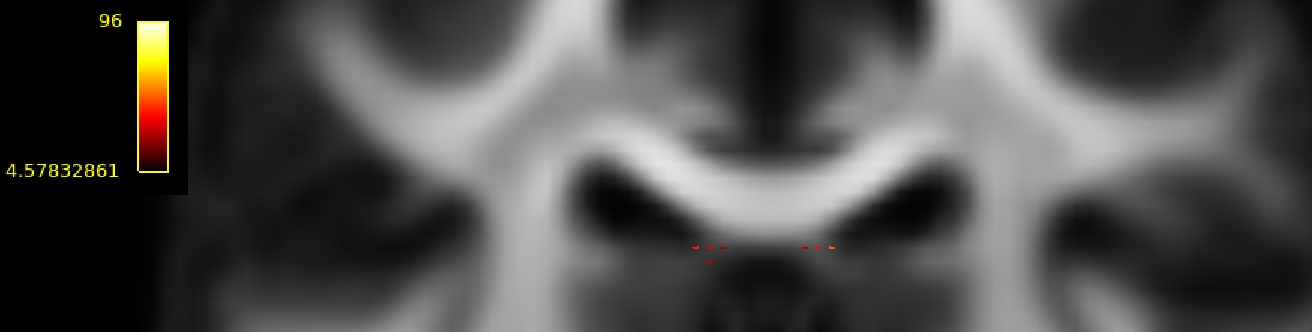
\includegraphics[width=0.8\linewidth]{Images/comp_TDI2.jpg}
        \label{fig:subfig-full-fixel}
    }
    \caption{Fixels extracted with MT-CSD, testing for an increase in AFD in the CP group compared to HC. Significant fixels are shown and colored by percentage increase relative to the mean value in the HC group. (a) Results after reducing the number of fixels by excluding low-density fixels. (b) Original results. Reducing the number of fixels increases statistical power, revealing additional effects, particularly near the CC.}
    \label{fig:reduced_MT}
\end{figure}


For LoRE-SD ODFs scaled with the intra-axonal contrast, applying the streamline threshold (250) reduced the total number of fixels from 320,964 to 196,217. In this case, 66 fixels were found significant for AFD when testing for increased values in CP vs. HC. These included new fixels in the fornix and CC as shown in Figure~\ref{fig:reduced_intra}. Furthermore, additional significant fixels emerged within regions previously identified in the analysis with the full fixel mask.

\begin{figure}[H]
    \centering
    \subfloat[]{
        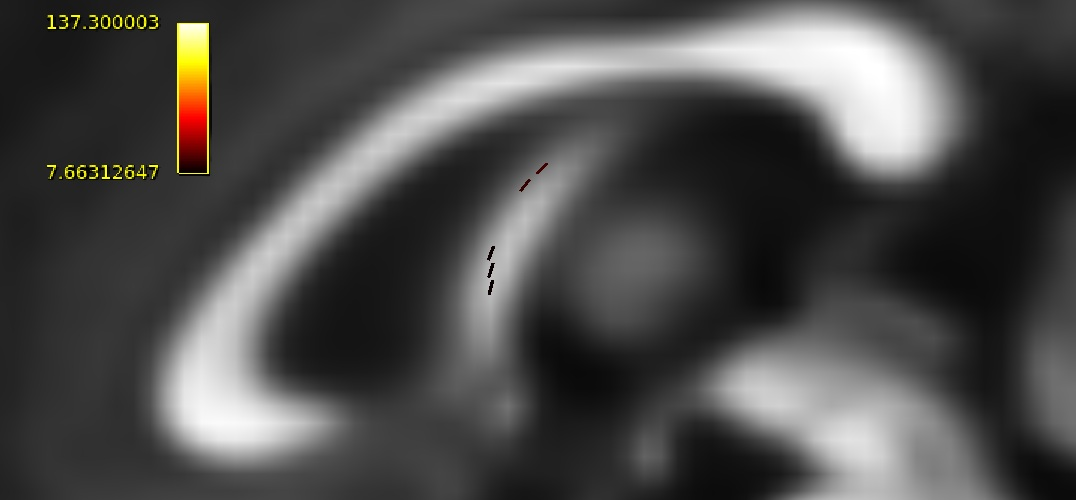
\includegraphics[width=0.5\linewidth]{Images/intra_TDI1.jpg}
        \label{fig:subfig-intra-A}
    }
    \hfill
    \subfloat[]{
        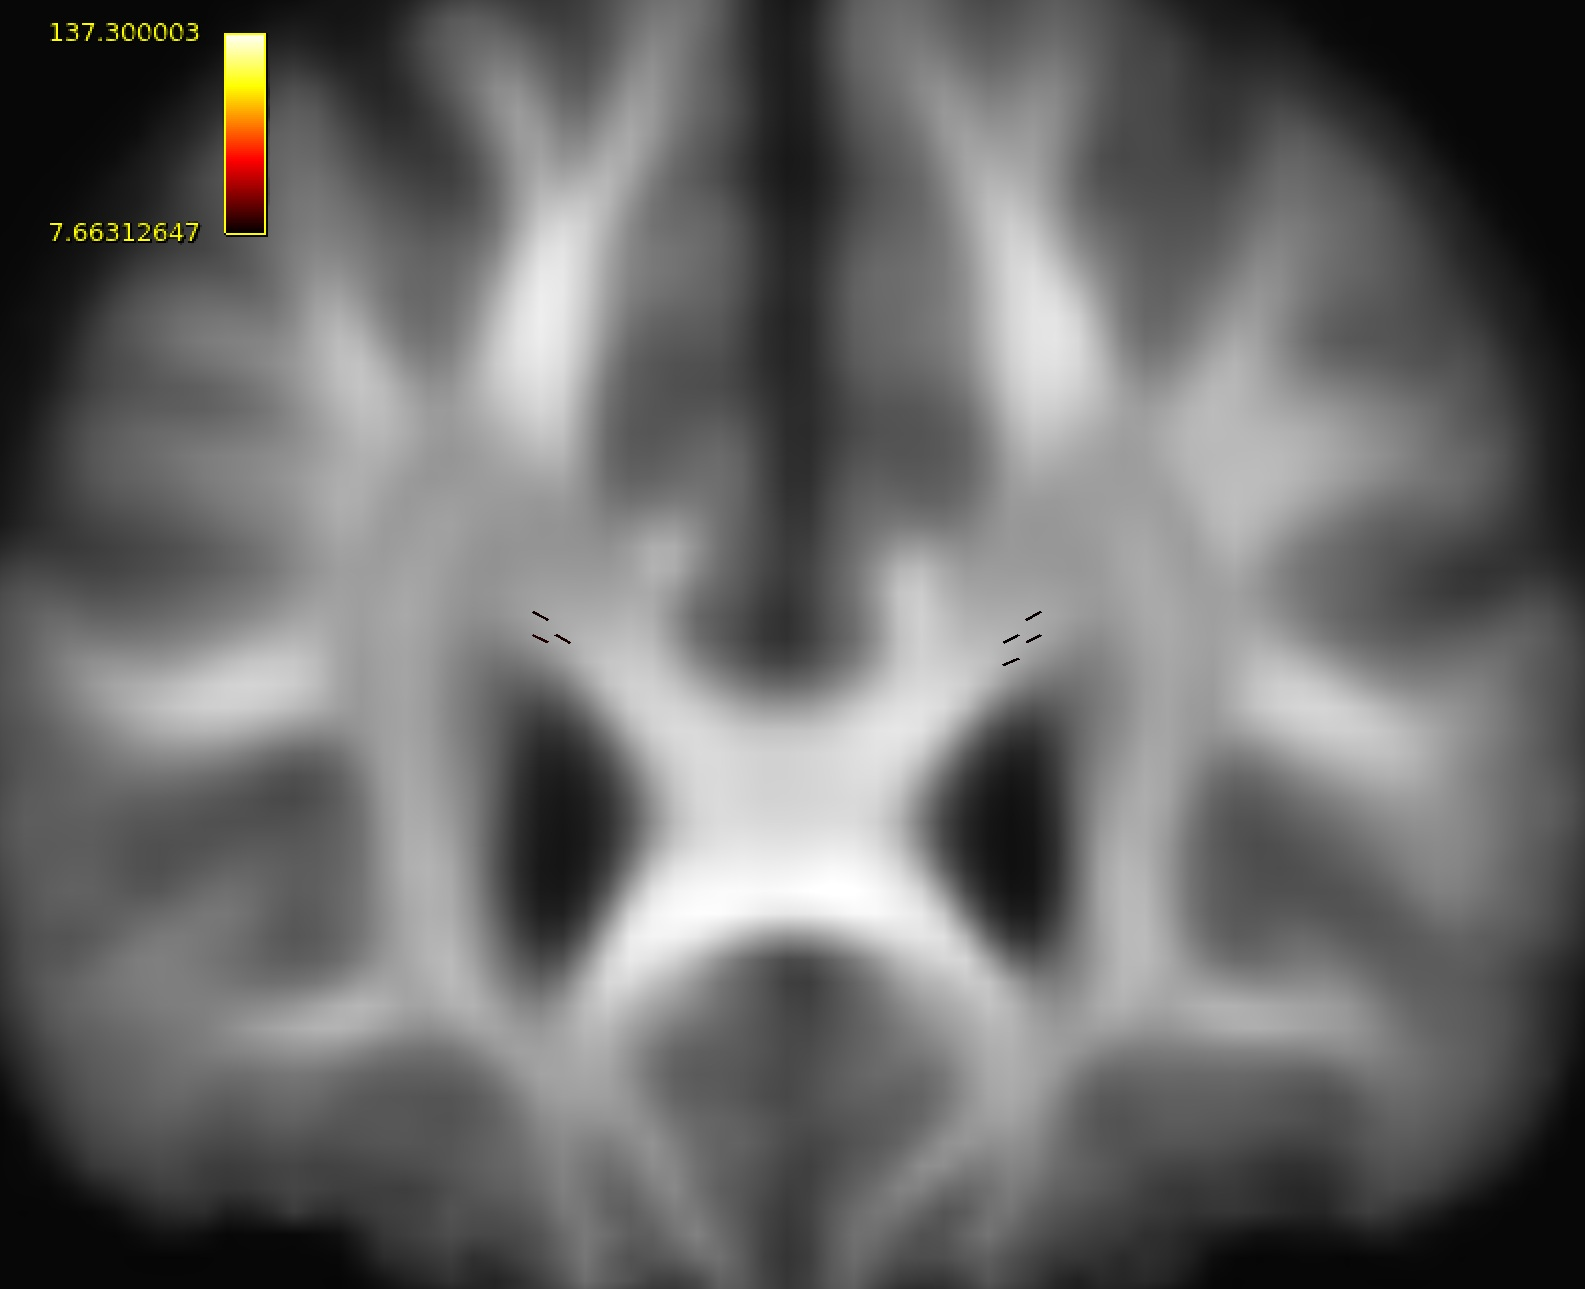
\includegraphics[width=0.5\linewidth]{Images/intra_TDI2.jpg}
        \label{fig:subfig-intra-B}
    }
    \caption{Fixels extracted from LoRE-SD scaled with the intra-axonal contrast, testing for higher AFD in CP compared to HC using the reduced fixel mask. Compared to the full mask results, new significant fixels are detected in the fornix (a) and near the genu of the corpus callosum (b). Only significant fixels are shown, colored by percentage increase relative to HC.}
    \label{fig:reduced_intra}
\end{figure}


With the FA scaling contrast, no significant fixels were detected even after applying the reduced fixel mask.
However, using the WM contrast, 162 fixels showed a significant increase in AFD in the CP group compared to HC. These fixels were in the regions identified in the original analysis.




\chapter{Discussion}
This chapter examines the application of LoRE-SD to FBA, highlighting how different ODF scaling contrasts affect results. We discuss how LoRE-SD’s flexibility can influence statistical outcomes and potentially provide biologically meaningful metrics beyond MT-CSD. Group differences, including unexpected increases in apparent fibre density in chemotherapy patients, are discussed in the context of compensatory mechanisms, protective responses, and atrophy. Finally, study limitations and future directions are outlined.

\section{LoRE-SD scaling contrasts}
Results in section~\ref{sec:cont} show how LoRE-SD is able to generate contrasts using the response function representation. Figure~\ref{fig:contrast_combined} demonstrates how an ad-hoc definition of the intra-axonal contrast highlights the same basis functions as a data-driven estimation of WM volume fraction. Both show high values for columns corresponding to low $\lambda_{\perp}$, with weights rapidly decreasing as $\lambda_{\perp}$ increases. This similarity supports the use of the intra-axonal contrast, rather than relying on data-driven approaches based on volume fractions estimations.

In this work, we derived a WM contrast matrix by solving an optimization problem separately for each subject, resulting in subject-specific matrices used to scale the corresponding ODFs. A potentially more robust alternative would involve solving a single optimization problem using the data (Gaussian fractions and WM volume fractions from MT-CSD) from all subjects or a representative subset. The resulting matrix could then be used to scale ODFs across all subjects in a consistent manner.
Additionally, such a matrix would capture the characteristics of a WM response function, defining how to weight and combine Gaussian basis functions to represent WM, similar to the study-specific response function used in MT-CSD. Unlike MT-CSD, which requires recomputing the response function for each study, the contrast matrix approach could provide a reusable representation applicable across different FBA studies, independent of the b-values acquired in a given study.
\\Furthermore, the WM contrast matrix derived through optimization shows lower values compared to those manually defined (Figure~\ref{fig:contrast_combined}). In particular, while the other matrices span the full range from 0 to 1, the WM contrast matrix reaches a maximum of around 0.8 across individuals. This results in the ODFs scaled with the contrast derived from this matrix having lower amplitudes than in the other cases. While for MT-CSD and intra-axonal-scaled LoRE-SD, 0.07 was the chosen threshold to extract fixels (Section \ref{sec:extract}), when scaling with the WM contrast the threshold on the lobe amplitude had to be adjusted. To get a number of fixels on the order of 300,000, 0.03 was chosen.  These threshold choices could have had an impact on the results that might need future investigation. An alternative approach could involve normalizing the values of the WM contrast matrix to the range 0-1, which would allow the use of the same amplitude threshold as in the other cases. However, we expect that the results would not differ significantly and the chosen approach is likely comparable.


The most computationally demanding step in the FBA pipeline is the creation of a population template, which requires multiple iterations of image registration. Given the flexibility of LoRE-SD-derived ODFs, which can be scaled in various ways, we propose using a single template based on one contrast, and applying the same subject-to-template transformation for ODFs scaled using other contrasts. This is possible because the different ODFs are simply scaled versions of the same unit-normalized ODFs.
In our implementation, the intra-axonal scaled template was used as the common reference space and the same warps were used to transform images scaled using the anisotropic intra-axonal and WM contrasts.
Fixel-wise metrics were subsequently extracted by integrating ODF lobes. These metrics are analogous to AFD (e.g., intra-axonal-weighted AFD, FA-weighted AFD, etc.). The flexibility in the response function representation allows the derivation of these additional metrics that might have a biological meaning.

FBA was performed using various scaling contrasts for the ODFs. This procedure involves multiple steps and can be time-consuming, but after selecting suitable hyperparameters, the analysis was fully automated. A simpler alternative could involve performing a group comparison directly on the new contrasts obtained for each subject, without scaling the ODFs and conducting FBA. This approach would resemble voxel-based analysis (VBA), where differences are assessed voxel by voxel, but each voxel value would still reflect information from a specific tissue compartment and meaningful differences among subject could be found. Such an approach could be explored in future studies.

\section{Masks}
As mentioned in section~\ref{sec:mask}, a more stringent masking method was required for LoRE-SD compared to MT-CSD. This is because including voxels outside the brain led to highly noisy and disproportionately large SH coefficients in the scaled ODFs. These outliers resulted from regions with near-zero radial and axial diffusivity (e.g., air or skull). Specifically, for the intra-axonal contrast this resulted in really big scaling factors, due to having close to zero radial diffusivity. This was problematic especially during affine registration, as these big values completely guided the transformations leading to implausible shears and scalings. The SynthStrip mask couldn't exclude the outliers for all the subjects, even after erosion was applied. The method that uses tissues volume fractions, although relying on the results of MT-CSD, provides masks able to exclude all noisy ODFs (Figure~\ref{fig:mask}).
Alternative strategies could be used for brain tissue volume fraction estimation, for example using probabilistic models such as Gaussian mixture models \cite{zhang2001}.

\section{Impact of Different Representations}
Even though MT-CSD and LoRE-SD produced generally different results, some degree of overlap was observed. For example, the fornix was identified as a significant region when using MT-CSD-derived ODFs, and also when using LoRE-SD-derived ODFs, but only when the WM contrast (itself derived from MT-CSD) was applied. This suggests that the response function representation of LoRE-SD can be used to mimic the previous method, effectively capturing similar microstructural features.
Additionally, for LoRE-SD the results were sensitive to the choice of contrast scaling. Brain regions identified as significant with one scaling approach were not necessarily detected with others, indicating the flexibility of LoRE-SD. More importantly this shows how the outcome of FBA is affected by ODF modulation, something previously under investigated as only one scaling factor, the apparent WM volume fraction used in MT-CSD, was available.


\section{Chemobrain}
To account for potential confounding from psychological stress due to the diagnosis, a cancer control (CM) group was included. No significant differences were found between CM and HC, suggesting that stress alone is unlikely to cause detectable white matter changes. This supports the hypothesis that cognitive symptoms and structural alterations in chemotherapy patients (CP) may result from chemotherapy-induced neurotoxicity. Unexpectedly, an increase in AFD was observed in the CP group, mainly in regions associated with cognitive function, particularly the fornix.

Increases in fixel-wise metrics have been observed in other neurological conditions and have been interpreted as compensatory reorganization or protective responses to neuroinflammation (\cite{Verhelst2019,Andica2021}). In the fornix, a central pathway connecting the hippocampus with other memory-related regions which plays a key role in cognition and episodic memory recall(\cite{Li2022, Senova2020}), such changes may reflect adaptive remodeling aimed at maintaining cognitive function. 

Despite the increase in AFD, no significant changes were observed in FC or the combined metric FDC. This suggests that microstructural changes, such as altered axonal packing or diameter, may occur without modifying the macroscopic cross-sectional area or overall capacity of the fibre bundle. However the lack of FDC changes weakens the interpretation of a true structural reorganization and highlights the need to consider alternative explanations.

Technical factors may also contribute to the observed effects. The fornix is a very thin structure, approximately 3 mm in width \cite{Yucel2002}, making it particularly vulnerable to partial volume effects from adjacent cerebrospinal fluid as well as to misregistration across subjects. Atrophy of the fornix has been reported in conditions such as Alzheimer’s disease \cite{Ali2025}, and if similar changes occurred in our patients, they could further amplify these issues, producing apparent AFD increases that may not reflect genuine microstructural alterations. Similarly, regions near the ventricles are especially prone to such artifacts, underscoring the need for cautious interpretation.

In summary, the increase in AFD observed in the fornix may result either from true white matter reorganization or protective adaptation in response to chemotherapy-induced neurotoxicity, or from artifacts related to partial volume effects or misregistration. Regardless of the underlying mechanism, the involvement of the fornix is consistent with its critical role in cognition, linking the hippocampus to broader memory networks and potentially explaining the cognitive deficits observed in chemobrain.


\section{Improving Statistical Power by Reducing the Fixel Mask}
As expected, reducing the number of fixels through TDI-based thresholding increased the number of significant fixels in each test, likely due to improved statistical power. A region near the CC was more prominently identified than in the original fixel mask (Figure~\ref{fig:reduced_MT} and~\ref{fig:reduced_intra}). However, even with the reduced fixel mask, no regions were identified with significantly lower fixel-wise metrics in patients compared to controls.
A more targeted alternative could be to restrict the analysis to specific tracts of interest, such as the CC or superior longitudinal fasciculus. 
\\Notably, after reducing the fixel mask, the fornix emerged as a region showing increased AFD in the CP group compared to HC, even when using the intra-axonal contrast for ODF scaling, a result not observed with the original fixel mask.

\section{Limitations of the work}
The mechanisms of chemotherapy-induced WM damage and the spatial distribution of affected regions is not yet fully understood. If, as reported by Schroyen et al. \cite{Schroyen2023}, chemotherapy primary leads to the enlargement of existing lesions rather than the formation of new ones, this may result in spatially heterogeneous abnormalities. Such heterogeneity challenges the assumptions of voxel- or fixel-wise group comparisons, which rely on spatially consistent effects across individuals. This could explain the limited number of significant findings in our analysis, particularly why we found no decreases in fixel metrics in chemotherapy patients compared to healthy controls. Notably, previous studies investigating chemobrain in breast cancer patients using diffusion MRI-derived metrics have also reported inconsistent group-level differences. While some studies have found significant effects using DTI-based measures, group differences using FBA have not been found \cite{Deprez2011, Schroyen2021}.
\\Statistical analysis using Connectivity-Based Fixel Enhancement assumes that structurally connected axons are likely to undergo similar pathological changes. This assumption is used to enhance the statistical power of the analysis, mitigating the effects of correction for multiple comparisons. However, this spatial coherence assumption may also inflate results in some cases, as fixels might appear significant only due to their connection to truly affected regions, rather than real pathological changes. To some extent, this may have influenced certain findings in our analysis.
\\Additional limitations relate to the fixel-wise metrics themselves. Although these provide advantages over voxel-wise metrics by assigning values to specific fibre populations, the derived measures can still be influenced by changes in adjacent fibre populations or nonaxonal tissue compartments. These potential confounds complicate the biological interpretation as a priori knowledge about the mechanisms of the condition would be needed. For this reason, the observed increase in apparent fibre density cannot be directly interpreted as a true increase in axonal content.
\\ As the findings of this work have not previously been reported, replication in independent cohorts is necessary to confirm their robustness and further clarify the underlying biological processes.

\section{Future Developments}
Reducing the number of fixels led to increased spatial extent of significant findings but did not reveal new regions. An alternative strategy might involve a ROI-based analysis using predefined WM tracts from a template. However, given the limited knowledge about which WM tracts are most affected by chemotherapy, such a tract-restricted approach could be overly limiting. Still, focusing on WM regions related to cognition may be a valuable future direction, potentially allowing additional fixels to reach statistical significance.
\\Future work should also incorporate cognitive test scores to understand how they relate to the observed WM changes. Additionally, adopting a longitudinal study design would allow for tracking the progression of structural alterations and their relationship with cognitive outcomes over time.
\\Finally, considering the specific chemotherapy agents used could help identify differential neurotoxic effects, potentially informing more personalized treatment strategies.

Regarding the LoRE-SD method, additional work is needed to better understand the biological meaning, if any, of the metrics extracted using different scaling contrasts. In particular, applying LoRE-SD to a condition with well characterized pathological changes known to show certain effects in fixel-wise metrics using MT-CSD, could help validate and interpret these new metrics. Insights gained from such studies may provide a valuable foundation for investigating more complex conditions, such as chemobrain, where the underlying pathology is less well understood. Additionally, further exploration of scaling strategies for the ODFs, including the optimization to derive contrast matrices from existing contrasts, could help in the interpretability and robustness of LoRE-SD. 
\\Finally, in this work, scaling contrasts were designed to emphasize axonal properties, such as the intra-axonal compartment, fractional anisotropy, and white matter, allowing a direct comparison with MT-CSD, which derives metrics from the WM ODF scaled by WM volume fractions. However, the flexibility of LoRE-SD in highlighting different tissue compartments opens the possibility of developing contrasts that also capture extra-axonal contributions. Such contrasts could enable the extraction of additional metrics and potentially reveal significant effects, since chemotherapy may impact not only axons but also other tissue components. Further investigation will be required to determine whether such contrasts reveal meaningful group differences.





\chapter{Conclusion}
\label{ch:conclusions}%
In this thesis, we investigated the use of a new method, LoRE-SD, to derive ODFs from dMRI data. We did so by performing a group analysis to study the changes in white matter induced by chemotherapy in breast cancer patients. LoRE-SD proved to be a suitable method for FBA, offering valuable flexibility in how ODFs are scaled. The results were broadly consistent with those of the state-of-the-art MT-CSD. Importantly, we showed that FBA results depend not only on the ODFs themselves, but also on the way these ODFs are modulated. Specifically, with LoRE-SD, holding the ODF constant while varying the scaling contrast led to different outcomes. This highlights how applying multiple scaling contrasts allows to extract complementary information from the same data, potentially reflecting distinct tissue microstructural features.
\\Prior to the analysis, we hypothesized that chemotherapy-treated patients would show decreased fixel-wise metrics compared to untreated individuals, reflecting a loss of white matter integrity. Contrary to expectations, we observed significant increases in apparent fibre density, notably in the fornix, a tract associated with memory and cognitive functions. This finding may reflect compensatory mechanisms or structural reorganization in response to chemotherapy-induced inflammation, potentially manifesting as an increase in axon number in the fornix. Such neuroplastic changes might be the brain's adaptive response to inflammatory processes triggered by treatment.
However, the fornix and other significant regions are located near the ventricles, making them particularly susceptible to partial volume effects. In addition, because the fornix is a very thin structure, misregistration during spatial normalization could also contribute to the observed differences. \\Although FBA allowed us to detect these effects, interpreting them remains challenging. 
\\Further research is needed both to clarify the biological meaning of the metrics extracted with LoRE-SD and to confirm the robustness of the observed findings.

%-------------------------------------------------------------------------
%	BIBLIOGRAPHY
%-------------------------------------------------------------------------

\addtocontents{toc}{\vspace{2em}} % Add a gap in the Contents, for aesthetics
\bibliography{Thesis_bibliography} % The references information are stored in the file named "Thesis_bibliography.bib"

%-------------------------------------------------------------------------
%	APPENDICES
%-------------------------------------------------------------------------

\cleardoublepage
\addtocontents{toc}{\vspace{2em}} % Add a gap in the Contents, for aesthetics



% LIST OF FIGURES
\listoffigures

% LIST OF TABLES
\listoftables

% LIST OF SYMBOLS
% Write out the List of Symbols in this page
\chapter*{List of Abbreviations} % You have to include a chapter for your list of symbols (
\begin{table}[H]
    \centering
    \begin{tabular}{ll}
       % \textbf{Variable} & \textbf{Description} \\\hline\\[-9px]
        %$\bm{u}$ & solid displacement & m \\[2px]
        %$\bm{u}_f$ & fluid displacement & m \\[2px]
        ADC & Apparent Diffusion Coefficient\\
    AFD & Apparent Fibre Density\\
    BBB   & Blood-Brain Barrier \\
    CC & Corpus Callosum\\
    CFE & Connectivity-based Fixel Enhancement\\
    CM & Chemotherapy-Na\"ive Patients\\
    CNN & Convolutional Neural Network\\
    CP & Chemotherapy Patients\\
    CSD & Constrained Spherical Deconvolution\\
    CSF & Cerebrospinal Fluid\\
    dMRI   & Diffusion-weighted Magnetic Resonance Imaging \\
    DTI & Diffusion Tensor Imaging\\
    GM & Gray Matter \\
    FA & Fractional Anisotropy\\
    FBA & Fixel-Based Analysis\\
    FC & Fibre Cross-section\\
    FDC & Fibre Density and Cross-section\\
    FWE & Family-wise Error\\
    GLM & General Linear Model\\
    HARDI & High Angular Resolution Diffusion Imaging\\
    HC & Healthy Controls\\
    LoRE-SD & Local Response function Estimation in Spherical Deconvolution\\
    MD & Mean Diffusivity\\
   MT-CSD & Multi-tissue Constrained Spherical Deconvolution\\
   ODF & Orientation Distribution Function\\
   ROI & Region of Interest\\
   SH & Spherical Harmonics\\
   SNR & Signal-to-Noise Ratio\\
   TDI & Track-Density Imaging\\
      WM  & White Matter \\
      VBA & Voxel-Based Analysis
    \end{tabular}
\end{table}

% ACKNOWLEDGEMENTS
\chapter*{Acknowledgements}


\cleardoublepage

\end{document}
